\documentclass[a4paper,12pt,openany]{book}

\usepackage[utf8]{inputenc}
\usepackage[T1]{fontenc}
\usepackage[french]{babel}
\usepackage{graphicx}
\usepackage{fancyhdr}
\usepackage{mathrsfs}
\usepackage{array}
\usepackage{amsfonts}
\usepackage{amsmath}
\usepackage{amssymb}
\usepackage{epstopdf}
\usepackage{booktabs}
\usepackage{xcolor}
\usepackage{hyperref}
\usepackage{caption}
\usepackage{subcaption}
\usepackage{float}
\usepackage{geometry}
\usepackage{titlesec}
\usepackage{enumitem}
\usepackage{longtable}
\usepackage{multirow}
\usepackage{pgfplots}
\pgfplotsset{compat=1.18}
\usepackage{circuitikz}
\usepackage{tikz}
\usepackage{lscape}

\graphicspath{
	{assets/}
	{assets/composants/}
	{assets/datasheet/}
	{assets/schema/}
	{assets/pcb/}
	{assets/pspice/}
}

\geometry{a4paper, top=2.5cm, bottom=2.5cm, left=2.5cm, right=2.5cm}
\setcounter{secnumdepth}{3}
\setcounter{tocdepth}{3}

\hypersetup{colorlinks=true, linkcolor=blue!60!black,
	citecolor=green!50!black, urlcolor=blue}

\pagestyle{fancy}
\fancyhf{}
\fancyhead[L]{\small Mini Projet \'Electronique I -- Variateur MCC}
\fancyhead[R]{\small ENIT -- 1AGE}
\fancyfoot[C]{\thepage}
\renewcommand{\headrulewidth}{0.4pt}
\setlength{\headheight}{14.5pt}

\begin{document}
	
	%% ===== PAGE DE GARDE =====
	\frontmatter
	\thispagestyle{empty}
	
	\begin{tikzpicture}[remember picture, overlay]
		\draw[line width=2pt]
		([xshift=1cm, yshift=-1cm]current page.north west)
		rectangle
		([xshift=-1cm, yshift=1cm]current page.south east);
	\end{tikzpicture}
	
	\begin{center}
		\begin{minipage}[c]{0.18\linewidth}
			
\includegraphics[height=2.5cm]{utm-logo.png}
		\end{minipage}
		\hfill
		\begin{minipage}[c]{0.58\linewidth}
			\centering
			\textbf{\scriptsize R\'epublique Tunisienne}\\[3pt]
			\textbf{\scriptsize Minist\`ere de l'Enseignement Sup\'erieur}\\
			\textbf{\scriptsize et de la Recherche Scientifique}\\[3pt]
			\textbf{\scriptsize Universit\'e de Tunis El Manar}\\[3pt]
			\textbf{\scriptsize \'Ecole Nationale d'Ing\'enieurs de Tunis}
		\end{minipage}
		\hfill
		\begin{minipage}[c]{0.18\linewidth}
			\centering
			
\includegraphics[height=2.9cm]{enit-logo.png}
		\end{minipage}
		
		\vspace{0.8cm}
		{\large \textbf{D\'epartement G\'enie \'Electrique}}
		
		\vspace{1.5cm}
		{\LARGE \textbf{Mini Projet d'\'Electronique I}}
		
		\vspace{2cm}
		\noindent\rule{\linewidth}{1.5pt}\\[6pt]
		{\bf\LARGE Conception et R\'ealisation d'un Variateur de Vitesse\\[8pt]
			pour Moteur \`a Courant Continu}\\[6pt]
		\noindent\rule{\linewidth}{1.5pt}
		
		\vspace{2.5cm}
		{\Large \textbf{\'Elabor\'e par~:}}\\[10pt]
		{\Large \textbf{WASSIM TOUKEBRI}}\\[10pt]
		{\Large \textbf{Classe~: 1\textsuperscript{\`ere} Ann\'ee G\'enie \'Electrique 3}}
		
		\vspace{2cm}
		{\Large \textbf{Encadr\'e par~:}}\\[10pt]
		{\Large \textbf{M. Joseph Haggege}}\\[6pt]
		{\Large \textbf{M. Wissem Naouar}}
		
		\vfill
		{\textbf{Ann\'ee universitaire 2025/2026}}
	\end{center}
	
	%% ===== REMERCIEMENTS =====
	\newpage
	\thispagestyle{empty}
	\centerline{\Large \textbf{Remerciements}}
	\vspace{2\baselineskip}
	
	Nous tenons \`a remercier, dans un premier temps, toute l'\'equipe
	p\'edagogique de l'\'Ecole Nationale d'Ing\'enieurs de Tunis (ENIT) ainsi
	que les intervenants professionnels du d\'epartement de g\'enie
	\'electrique, pour avoir assur\'e la partie th\'eorique de ce mini-projet.
	
	Nous adressons \'egalement nos remerciements \`a \textbf{M. Joseph Haggege}
	et \textbf{M. Wissem Naouar} pour l'aide et les conseils pr\'ecieux qu'ils
	nous ont apport\'es lors des diff\'erents suivis concernant les missions
	\'evoqu\'ees dans ce rapport.
	
	Nous souhaitons exprimer notre gratitude particuli\`ere et t\'emoigner de
	toute notre reconnaissance aux techniciens responsables du laboratoire
	d'\'electronique, pour l'exp\'erience enrichissante et pleine d'int\'er\^et
	qu'ils nous ont fait vivre durant ce mini-projet.
	
	Enfin, nous remercions nos camarades de promotion pour l'entraide et la
	collaboration fructueuse tout au long de ce travail, et plus
	particuli\`erement \textbf{Jasser Mhamdi} pour son aide pr\'ecieuse et
	son soutien constant.
	
	%% ===== RÉSUMÉ =====
	\newpage
	\thispagestyle{empty}
	\centerline{\Large \textbf{R\'esum\'e}}
	\vspace{\baselineskip}
	
	Ce rapport pr\'esente la conception et la r\'ealisation d'un variateur de
	vitesse pour moteur \`a courant continu (MCC) sous forme de carte PCB.
	Le syst\`eme utilise une commande MLI g\'en\'er\'ee par un circuit
	\textbf{NE555N} en mode astable, dont le rapport cyclique est contr\^ol\'e
	par un potentiom\`etre. Un transistor MOSFET de puissance \textbf{IRF530}
	assure la commutation de l'alimentation du moteur. L'alimentation est
	fournie par une alimentation double sym\'etrique $\pm12$\,V \`a base des
	r\'egulateurs \textbf{7812} et \textbf{7912}, et d'une alimentation
	ajustable \textbf{LM317T}. Un amplificateur op\'erationnel \textbf{$\mu$A741P}
	et un comparateur \textbf{LM393N} assurent le conditionnement des signaux.
	Les fonctions marche/arr\^et et sens de rotation sont g\'er\'ees par des
	bascules JK (\textbf{CD4027N}). La conception a \'et\'e r\'ealis\'ee sous
	EAGLE et valid\'ee par simulation PSpice.
	
	\noindent \textbf{Mots cl\'es~:} Variateur MCC, MLI, NE555N, IRF530,
	LM317T, 7812, 7912, $\mu$A741P, LM393N, CD4027N, Eagle, PSpice
	
	\vspace{2\baselineskip}
	\centerline{\Large \textbf{Abstract}}
	\vspace{\baselineskip}
	
	This report presents the design and implementation of a PCB-based DC motor
	speed controller. The system employs PWM generated by a \textbf{NE555N}
	timer in astable mode with an adjustable duty cycle. A power MOSFET
	\textbf{IRF530} handles motor power switching. The power supply is a dual
	$\pm12$\,V using \textbf{7812} and \textbf{7912} fixed regulators and an
	adjustable \textbf{LM317T}. An op-amp \textbf{$\mu$A741P} and comparator
	\textbf{LM393N} handle signal conditioning. Start/stop and direction control
	are managed by JK flip-flops (\textbf{CD4027N}). The design was produced in
	EAGLE and validated by PSpice simulation.
	
	\noindent \textbf{Key Words~:} DC motor controller, PWM, NE555N, IRF530,
	LM317T, 7812, 7912, $\mu$A741P, LM393N, CD4027N, Eagle, PSpice
	
	%% ===== TABLE DES MATIÈRES =====
	\tableofcontents
	\newpage
	\addcontentsline{toc}{chapter}{\listfigurename}
	\listoffigures
	\newpage
	\addcontentsline{toc}{chapter}{\listtablename}
	\listoftables
	
	%% ===== INTRODUCTION =====
	\chapter*{Introduction}
	\addcontentsline{toc}{chapter}{Introduction}
	\markboth{Introduction}{Introduction}
	
	Ce rapport pr\'esente les \'etapes de conception et de r\'ealisation d'un
	variateur de vitesse pour moteur \`a courant continu (MCC) sous forme de
	carte \'electronique. Le processus inclut la saisie du sch\'ema sous EAGLE,
	la simulation des blocs sous PSpice et la fabrication de la carte. Ce
	travail s'inscrit dans le cadre du Mini Projet d'\'Electronique I \`a
	l'\'Ecole Nationale d'Ing\'enieurs de Tunis (ENIT).
	
	\bigskip\noindent\textbf{Probl\'ematique}
	
	Comment concevoir et r\'ealiser efficacement un variateur de vitesse pour
	moteur \`a courant continu, en int\'egrant des m\'ethodes de conception
	assist\'ee par ordinateur et de simulation num\'erique, tout en garantissant
	des performances optimales~?
	
	\bigskip
	Ce rapport est structur\'e en trois chapitres~:
	\begin{itemize}
		\item \textbf{Chapitre 1 -- Outils et Pr\'erequis~:} pr\'esentation des
		logiciels (EAGLE, PSpice) et des composants \'electroniques utilis\'es.
		\item \textbf{Chapitre 2 -- \'Etude Th\'eorique~:} analyse des blocs
		fonctionnels et simulations PSpice.
		\item \textbf{Chapitre 3 -- R\'ealisation~:} fabrication et tests de la
		carte \'electronique finale.
	\end{itemize}
	
	\mainmatter
	
	%%=========================================================
	\chapter{Outils et Pr\'erequis}
	
	\section{Logiciels}
	
	\subsection{EAGLE}
	
	EAGLE~\cite{EAGLE} est un logiciel de conception \'electronique assist\'ee
	par ordinateur (CAO) utilis\'e pour~:
	\begin{itemize}
		\item cr\'eer des sch\'emas \'electriques,
		\item placer et router les composants sur le PCB,
		\item g\'en\'erer les fichiers de fabrication (Gerber).
	\end{itemize}
	
	\subsection{PSpice}
	
	PSpice~\cite{PSPICE} est un logiciel de simulation de circuits
	\'electroniques d\'evelopp\'e par Cadence Design Systems, permettant de
	valider le comportement des circuits avant leur fabrication physique.
	
	\section{Composants \'Electroniques}
	
	\subsection{NE555N -- Minuterie/Oscillateur}
	
	Le \textbf{NE555N}~\cite{NE555DS} (IC3) est un circuit int\'egr\'e de
	temporisation monolithique introduit en 1972, devenu une r\'ef\'erence
	universelle pour les applications d'oscillation et de chronom\'etrage.
	Il est utilis\'e dans notre circuit en \textbf{mode astable} pour
	g\'en\'erer le signal de porteuse (signal triangulaire) servant \`a
	la g\'en\'eration du signal MLI.
	
	\begin{figure}[H]
		\centering
		\begin{subfigure}[b]{0.45\textwidth}
			\centering
			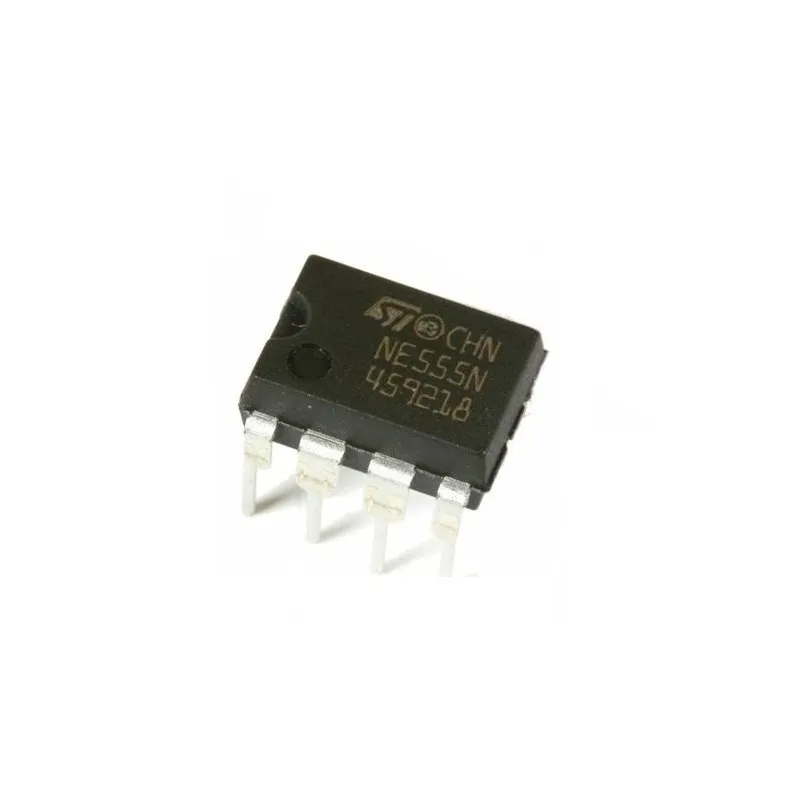
\includegraphics[width=\textwidth]{ne555_photo}
			\caption{Circuit NE555N (DIP-8)}
		\end{subfigure}
		\hfill
		\begin{subfigure}[b]{0.50\textwidth}
			\centering
			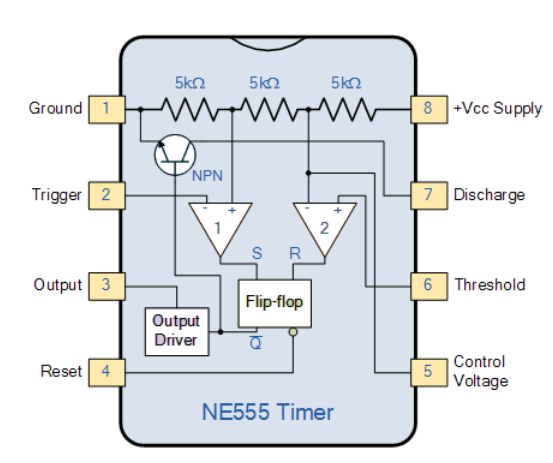
\includegraphics[width=\textwidth]{ne555_brochage}
			\caption{Brochage du NE555N}
		\end{subfigure}
		\caption{Circuit int\'egr\'e NE555N}
		\label{fig:ne555}
	\end{figure}
	
	\subsubsection{Structure interne}
	
	Le NE555N contient quatre blocs fonctionnels principaux~:
	\begin{itemize}
		\item \textbf{Deux comparateurs de tension~:} le premier compare
		la tension de TRIG avec $\frac{1}{3}V_{cc}$~; le second
		compare THR avec $\frac{2}{3}V_{cc}$.
		\item \textbf{Une bascule RS~:} m\'emorise l'\'etat de sortie
		en fonction des comparateurs.
		\item \textbf{Un transistor de d\'echarge~:} connecte la broche
		DISCH \`a la masse pour d\'echarger le condensateur externe.
		\item \textbf{Un \'etage de sortie~:} capable de fournir ou
		d'absorber jusqu'\`a 200\,mA.
	\end{itemize}
	
	\subsubsection{Brochage}
	
	\begin{table}[H]
		\centering
		\caption{Brochage du NE555N (DIP-8)}
		\begin{tabular}{|c|l|l|}
			\hline
			\textbf{Pin} & \textbf{Nom} & \textbf{Fonction} \\
			\hline
			1 & GND   & Masse \\
			2 & TRIG  & D\'eclenchement (seuil $\frac{1}{3}V_{cc}$) \\
			3 & OUT   & Sortie (0 ou $V_{cc}$, courant max 200\,mA) \\
			4 & RESET & R\'einitialisation (actif bas, reli\'e \`a $V_{cc}$ si inutilis\'e) \\
			5 & CONT  & Tension de contr\^ole (acc\`es au pont diviseur interne) \\
			6 & THR   & Seuil haut ($\frac{2}{3}V_{cc}$) \\
			7 & DISCH & D\'echarge du condensateur externe \\
			8 & $V_{cc}$ & Alimentation (+5\,V \`a +15\,V) \\
			\hline
		\end{tabular}
		\label{tab:ne555_pins}
	\end{table}
	
	\subsubsection{Mode Astable et G\'en\'eration du Signal}
	
	En mode astable, le NE555N fonctionne comme un oscillateur libre.
	Le condensateur $C_4$ se charge \`a travers $R_A$ et $R_B$, puis se
	d\'echarge \`a travers $R_B$ uniquement via la broche DISCH. Les
	diodes D5 et D6 (1N4148) orientent s\'epar\'ement les courants de
	charge et de d\'echarge, produisant un signal quasi-triangulaire.
	
	La fr\'equence d'oscillation est donn\'ee par~:
	\begin{equation}
		f = \frac{1.44}{(R_A + 2R_B) \cdot C}
	\end{equation}
	
	Le rapport cyclique est~:
	\begin{equation}
		\alpha = \frac{R_A + R_B}{R_A + 2R_B}
	\end{equation}
	
	o\`u dans notre circuit~: $R_9 = 470\,\Omega$ ($R_A$),
	$R_6 = 10\,\text{k}\Omega$ ($R_B$) et $C_4 = 10\,\text{nF}$.
	
	\noindent Application num\'erique~:
	\begin{equation}
		f = \frac{1.44}{(470 + 2 \times 10\,000) \times 10 \times 10^{-9}}
		\approx \mathbf{7\,kHz}
	\end{equation}
	
	\subsubsection{Caract\'eristiques Principales}
	
	\begin{table}[H]
		\centering
		\caption{Caract\'eristiques \'electriques du NE555N
			(extrait datasheet~\cite{NE555DS})}
		\begin{tabular}{|l|c|c|c|}
			\hline
			\textbf{Param\`etre} & \textbf{Min.} & \textbf{Typ.}
			& \textbf{Max.} \\
			\hline
			Tension d'alimentation $V_{cc}$      & 4.5\,V & --    & 16\,V   \\
			Courant de sortie max                & --     & --    & 200\,mA \\
			Courant d'alimentation ($V_{cc}=5$\,V) & --   & 3\,mA & 6\,mA  \\
			Temp\'erature de fonctionnement      & 0\,\textdegree C & -- &
			70\,\textdegree C \\
			Pr\'ecision de temporisation         & --     & 1\,\% & --      \\
			Fr\'equence maximale                 & --     & --    & 300\,kHz \\
			\hline
		\end{tabular}
		\label{tab:ne555_specs}
	\end{table}
	

	
	
	
	
	%%----------------------------------------------------------
	\subsection{LM393N -- Comparateur de Tension Double}
	
	Le \textbf{LM393N}~\cite{LM393DS} (IC6) est un double comparateur de
	tension \`a sortie collecteur ouvert, utilis\'e pour comparer le signal de
	retour avec une r\'ef\'erence et g\'en\'erer un signal de protection.
	
	\begin{figure}[H]
		\centering
		\begin{subfigure}[b]{0.45\textwidth}
			\centering
			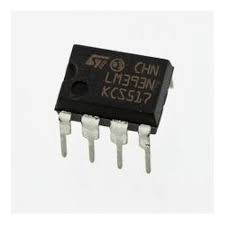
\includegraphics[width=\textwidth]{lm393_photo}
			\caption{Circuit LM393N (DIP-8)}
		\end{subfigure}
		\hfill
		\begin{subfigure}[b]{0.50\textwidth}
			\centering
			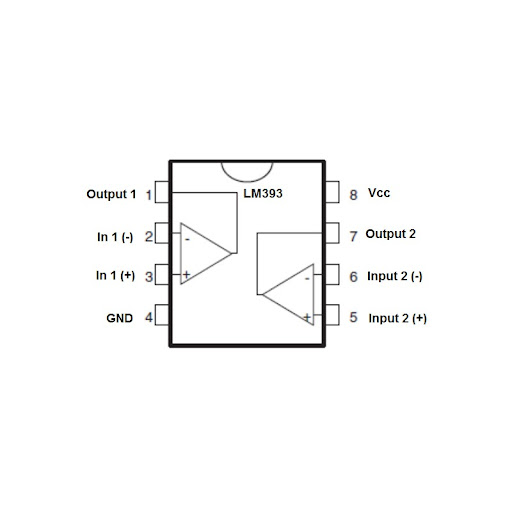
\includegraphics[width=\textwidth]{lm393_brochage}
			\caption{Brochage du LM393N}
		\end{subfigure}
		\caption{Circuit int\'egr\'e LM393N}
		\label{fig:lm393}
	\end{figure}
	
	\noindent Broches principales~:
	\begin{itemize}
		\item \textbf{Pin 1~:} Sortie 1 \quad \textbf{Pin 7~:} Sortie 2
		\item \textbf{Pin 2~:} Entr\'ee ($-$) 1 \quad \textbf{Pin 6~:} Entr\'ee ($-$) 2
		\item \textbf{Pin 3~:} Entr\'ee ($+$) 1 \quad \textbf{Pin 5~:} Entr\'ee ($+$) 2
		\item \textbf{Pin 4~:} GND \quad \textbf{Pin 8~:} $V_{cc}$
	\end{itemize}
	
	%%----------------------------------------------------------
	\subsection{$\mu$A741P -- Amplificateur Op\'erationnel}
	
	Le \textbf{$\mu$A741P}~\cite{UA741DS} (IC1) est un amplificateur
	op\'erationnel g\'en\'eral d'usage universel. Dans notre carte, il est
	utilis\'e comme conditionneur de signal pour la consigne de vitesse.
	Sa sortie est reli\'ee au pont diviseur (RV1, R2, R3) pour fournir la
	tension de r\'ef\'erence au NE555N.
	
	\begin{table}[H]
		\centering
		\caption{Caract\'eristiques principales du $\mu$A741P}
		\begin{tabular}{|l|c|c|}
			\hline
			\textbf{Param\`etre} & \textbf{Valeur typique} & \textbf{Unit\'e} \\
			\hline
			Tension d'alimentation max  & $\pm18$  & V      \\
			Gain en boucle ouverte      & 200\,000 & V/V    \\
			Bande passante (GBW)        & 1        & MHz    \\
			Slew Rate                   & 0.5      & V/$\mu$s \\
			\hline
		\end{tabular}
		\label{tab:ua741}
	\end{table}
	
	\begin{figure}[H]
		\centering
		\begin{subfigure}[b]{0.3\textwidth}
			\centering
			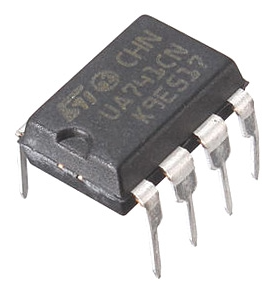
\includegraphics[width=\linewidth, height=0.5\textheight, keepaspectratio]{ua741_photo}
					\vspace{0.5cm}
			\caption{$\mu$A741P (DIP-8)}
		\end{subfigure}
		\hfill
		\begin{subfigure}[b]{0.50\textwidth}
			\centering
					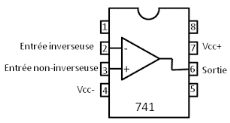
\includegraphics[width=\linewidth, height=0.92\textheight, keepaspectratio]{ua741_brochage}
					\vspace{0.5cm}
			\caption{Brochage du $\mu$A741P}
		\end{subfigure}
		\caption{Amplificateur op\'erationnel $\mu$A741P}
		\label{fig:ua741}
	\end{figure}
	
	%%----------------------------------------------------------
	\subsection{LM317T -- R\'egulateur Ajustable}
	
	Le \textbf{LM317T}~\cite{LM317DS} (IC2) est un r\'egulateur de tension
	positive ajustable \`a trois broches, capable de fournir jusqu'\`a 1.5\,A
	sur une plage de 1.2\,V \`a 37\,V. La tension de sortie est fix\'ee par~:
	\begin{equation}
		V_{out} \approx 1.25 \left(1 + \frac{R_{V2}}{R_4}\right)
	\end{equation}
	o\`u $R_4 = 1\,\text{k}\Omega$ et $R_{V2} = 470\,\Omega$.
	
	\begin{figure}[H]
		\centering
		\begin{subfigure}[b]{0.45\textwidth}
			\centering
			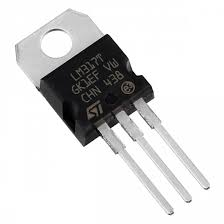
\includegraphics[width=0.7\linewidth, height=0.7\textheight, keepaspectratio]{lm317_photo}
					\vspace{0.5cm}
			\caption{LM317T (TO-220)}
		\end{subfigure}
		\hfill
		\begin{subfigure}[b]{0.50\textwidth}
			\centering
			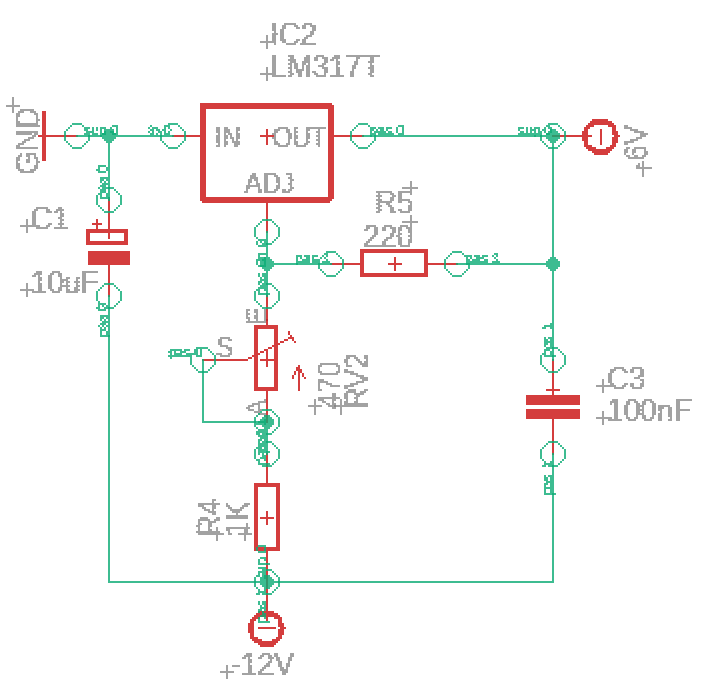
\includegraphics[width=1\linewidth, height=\textheight, keepaspectratio]{lm317_circuit}
					\vspace{0.5cm}
			\caption{Circuit r\'egulateur ajustable}
		\end{subfigure}
		\caption{R\'egulateur ajustable LM317T}
		\label{fig:lm317}
	\end{figure}
	
	%%----------------------------------------------------------
	\subsection{7812 et 7912 -- R\'egulateurs Fixes}
	
	Les r\'egulateurs \textbf{7812} (IC4) et \textbf{7912} (IC5) fournissent
	respectivement $+12$\,V et $-12$\,V stabilis\'es pour alimenter l'ensemble
	des circuits de commande.
	
	\begin{table}[H]
		\centering
		\caption{Caract\'eristiques des r\'egulateurs 7812 et 7912}
		\begin{tabular}{|l|c|c|c|}
			\hline
			\textbf{Param\`etre} & \textbf{7812} & \textbf{7912} & \textbf{Unit\'e} \\
			\hline
			Tension de sortie     & $+12$  & $-12$  & V \\
			Courant max           & 1.5    & 1.5    & A \\
			Tension d'entr\'ee min & 14.5  & $-14.5$ & V \\
			\hline
		\end{tabular}
		\label{tab:7812}
	\end{table}
	
	\begin{figure}[H]
		\centering
		\begin{subfigure}[b]{0.45\textwidth}
			\centering
			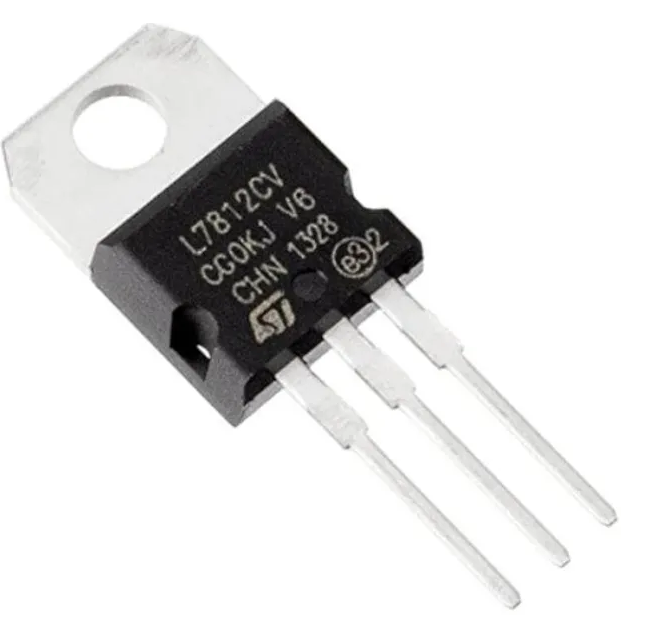
\includegraphics[width= 0.75\linewidth, height=0.4\textheight, keepaspectratio]{7812_photo}
					\vspace{0.1cm}
			\caption{R\'egulateur 7812 ($+12$\,V, TO-220)}
		\end{subfigure}
		\hfill
		\begin{subfigure}[b]{0.45\textwidth}
			\centering
			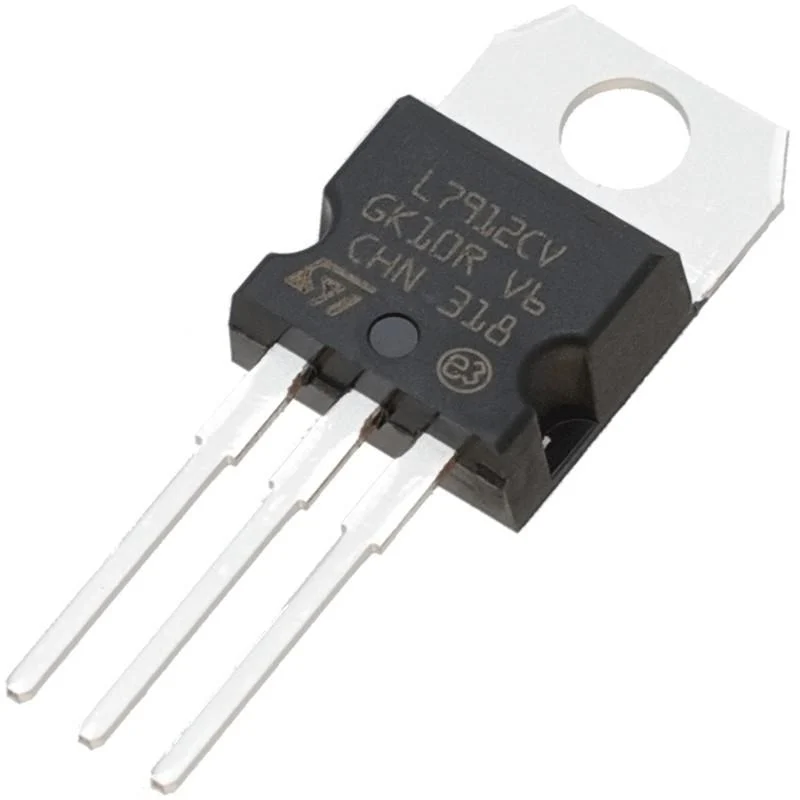
\includegraphics[width=\linewidth, height=0.2\textheight, keepaspectratio]{7912_photo}
					\vspace{0.5cm}\\
			\caption{R\'egulateur 7912 ($-12$\,V, TO-220)}
		\end{subfigure}
		\caption{R\'egulateurs de tension fixes 7812 et 7912}
		\label{fig:7812}
	\end{figure}
	
	%%----------------------------------------------------------
	\subsection{CD4027N -- Double Bascule JK}
	
	Le \textbf{CD4027N}~\cite{CD4027DS} (IC7) est un circuit CMOS contenant
	deux bascules JK ma\^itre-esclave ind\'ependantes. Les deux bascules
	(IC7A et IC7B) assurent respectivement~:
	\begin{itemize}
		\item \textbf{IC7A~:} la fonction \textbf{marche/arr\^et} (bouton S1),
		\item \textbf{IC7B~:} la commande du \textbf{sens de rotation} (bouton S2)
		via le relais K1 (G2R-2).
	\end{itemize}
	
	\begin{table}[H]
		\centering
		\caption{Table de v\'erit\'e de la bascule JK}
		\begin{tabular}{|c|c|c|c|}
			\hline
			\textbf{J} & \textbf{K} & \textbf{Q(t+1)} & \textbf{Fonction} \\
			\hline
			0 & 0 & Q(t)              & M\'emorisation \\
			0 & 1 & 0                 & Remise \`a z\'ero \\
			1 & 0 & 1                 & Mise \`a un \\
			1 & 1 & $\overline{Q(t)}$ & Basculement \\
			\hline
		\end{tabular}
		\label{tab:jk}
	\end{table}
	
	\begin{figure}[H]
		\centering
		\begin{subfigure}[b]{0.45\textwidth}
			\centering
			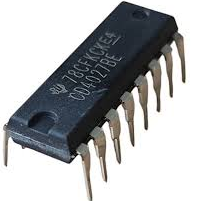
\includegraphics[width= 0.65\linewidth, height=0.4\textheight, keepaspectratio]{cd4027_photo}
					\vspace{0.5cm}
			\caption{CD4027N (DIP-16)}
		\end{subfigure}
		\hfill
		\begin{subfigure}[b]{0.50\textwidth}
			\centering
			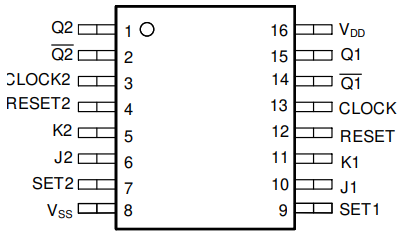
\includegraphics[width= 0.9\linewidth, height=0.6\textheight, keepaspectratio]{cd4027_brochage}
					\vspace{0.5cm}
			\caption{Brochage du CD4027N}
		\end{subfigure}
		\caption{Double bascule JK CD4027N}
		\label{fig:cd4027}
	\end{figure}
	
	%%----------------------------------------------------------
	\subsection{IRF530 -- MOSFET de Puissance}
	
	Le \textbf{IRF530}~\cite{IRF530DS} (Q6) est un transistor MOSFET de
	puissance de type N en bo\^itier TO-220. C'est l'\'el\'ement de commutation
	principal du variateur~: il re\c coit le signal MLI en entr\'ee de grille
	et commute le courant du moteur.
	
	\begin{table}[H]
		\centering
		\caption{Caract\'eristiques du MOSFET IRF530}
		\begin{tabular}{|l|c|c|}
			\hline
			\textbf{Param\`etre} & \textbf{Valeur} & \textbf{Unit\'e} \\
			\hline
			$V_{DSS}$ max            & 100  & V        \\
			$I_D$ continu            & 14   & A        \\
			$R_{DS(on)}$ typ.        & 0.16 & $\Omega$ \\
			$V_{GS(th)}$             & 2--4 & V        \\
			Puissance dissip\'ee max & 75   & W        \\
			\hline
		\end{tabular}
		\label{tab:irf530}
	\end{table}
	
	\begin{figure}[H]
		\centering
		\begin{subfigure}[b]{0.45\textwidth}
			\centering
			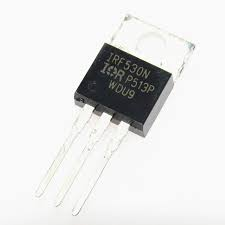
\includegraphics[width= 0.65\linewidth, height=0.4\textheight, keepaspectratio]{irf530_photo}
					\vspace{0.5cm}
			\caption{IRF530 (TO-220)}
		\end{subfigure}
		\hfill
		\begin{subfigure}[b]{0.50\textwidth}
			\centering
			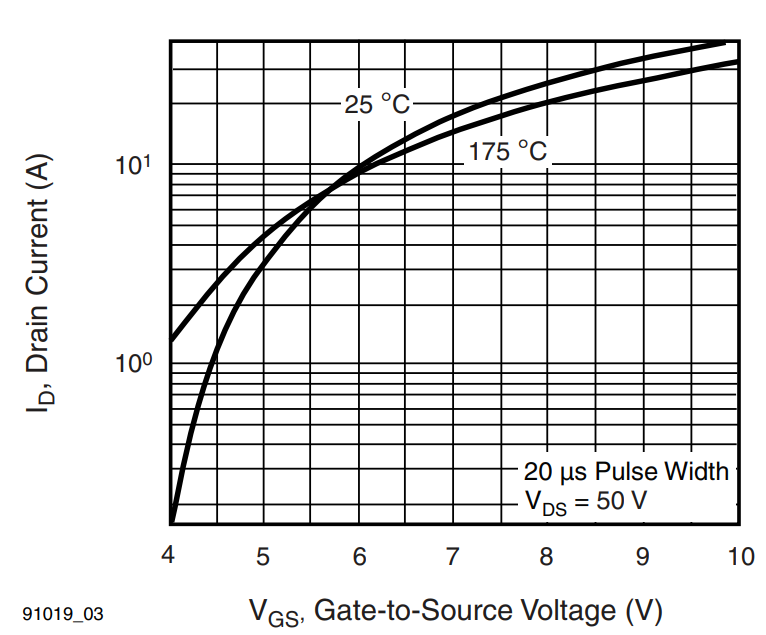
\includegraphics[width= 0.9\linewidth, height=0.9\textheight, keepaspectratio]{irf530_transfer}
					\vspace{0.5cm}
			\caption{Courbe $I_D = f(V_{GS})$}
		\end{subfigure}
		\caption{MOSFET de puissance IRF530}
		\label{fig:irf530}
	\end{figure}
	
	
	
	%%----------------------------------------------------------
	
	
	\subsection{Relais G2R-2 -- Inversion du Sens de Rotation}
	
	Le relais \textbf{G2R-2} (K1) est un relais \'electromagn\'etique double
	p\^ole double jet\'ee (DPDT) de la gamme Omron, aliment\'e en 12\,V DC.
	Il est utilis\'e dans notre circuit pour \textbf{inverser la polarit\'e}
	de la tension appliqu\'ee aux bornes du moteur MCC, permettant ainsi
	l'inversion du sens de rotation.
	
	\noindent Caract\'eristiques principales~:
	\begin{itemize}
		\item Tension de bobine~: 12\,V DC
		\item Courant de bobine~: 26.1\,mA
		\item Puissance de bobine~: 400\,mW
		\item Capacit\'e de commutation~: 5\,A / 250\,V AC
		\item Configuration~: DPDT (Double Pole Double Throw)
		\item Bo\^itier~: G2R2 (montage sur PCB)
	\end{itemize}
	
	\begin{figure}[H]
		\centering
		\begin{subfigure}[b]{0.45\textwidth}
			\centering
			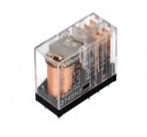
\includegraphics[width= 0.65\linewidth, height=0.4\textheight, keepaspectratio]{relais_photo}
				\vspace{0.5cm}
			\caption{Relais G2R-2 (Omron)}
		\end{subfigure}
		\hfill
		\begin{subfigure}[b]{0.50\textwidth}
			\centering
			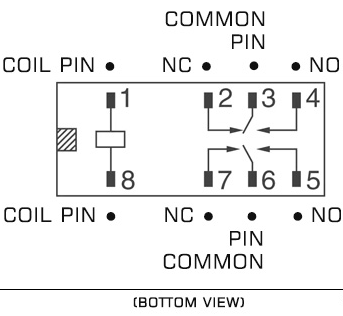
\includegraphics[width= 0.65\linewidth, height=0.4\textheight, keepaspectratio]{g2r2_schema}
				\vspace{0.5cm}
			\caption{Sch\'ema interne DPDT}
		\end{subfigure}
		\caption{Relais G2R-2 Omron -- commutation du sens de rotation}
		\label{fig:g2r2}
	\end{figure}
	
	\noindent Principe de fonctionnement dans le circuit~:
	\begin{itemize}
		\item \textbf{Bobine d\'esactiv\'ee (Q=0 de IC7B)~:} le moteur tourne
		dans le sens direct.
		\item \textbf{Bobine activ\'ee (Q=1 de IC7B)~:} le transistor 2N2222
		(Q7) sature et alimente la bobine du relais~; les contacts DPDT
		s'inversent, inversant la polarit\'e aux bornes du moteur.
	\end{itemize}
	
	
	%%----------------------------------------------------------
	\subsection{Transistors Bipolaires (BC547, BC557, 2N2222)}
	
	Les transistors \textbf{BC547} (Q3, Q5, NPN) et \textbf{BC557} (Q1, Q2,
	Q4, PNP) en bo\^itier TO-92 assurent les \'etages de commande logique entre
	les bascules JK et la grille du MOSFET IRF530. Le transistor
	\textbf{2N2222} (Q7) pilote le relais K1 (G2R-2) pour l'inversion du sens
	de rotation.
	
	\begin{figure}[H]
		\centering
		\begin{subfigure}[b]{0.30\textwidth}
			\centering
			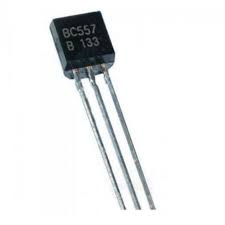
\includegraphics[width= 0.7\linewidth, height=0.7\textheight, keepaspectratio]{bc557}
					\vspace{0.5cm}
			\caption{BC547 NPN (TO-92)}
		\end{subfigure}
		\hfill
		\begin{subfigure}[b]{0.30\textwidth}
			\centering
		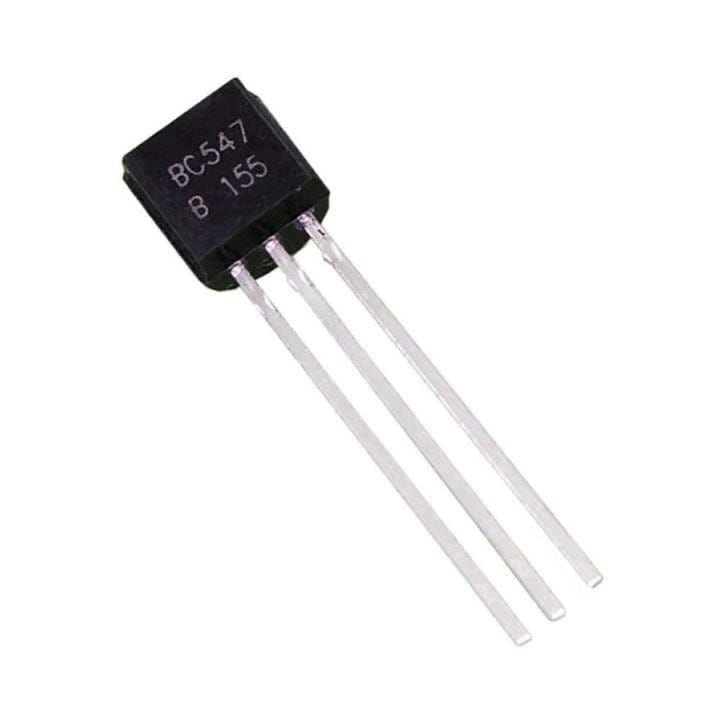
\includegraphics[width= 0.8\linewidth, height=0.8\textheight, keepaspectratio]{bc547}
				\vspace{0.5cm}
			\caption{BC557 PNP (TO-92)}
		\end{subfigure}
		\hfill
		\begin{subfigure}[b]{0.30\textwidth}
			\centering
		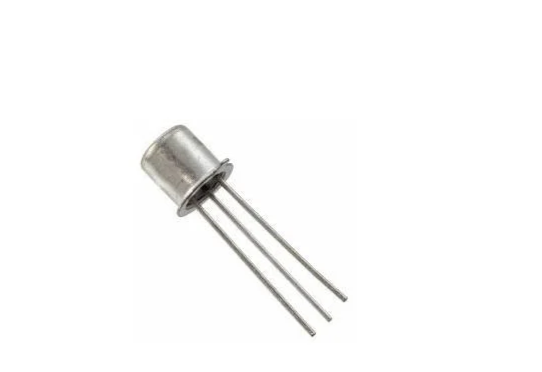
\includegraphics[width= 1\linewidth, height=1\textheight, keepaspectratio]{2n2222}
					\vspace{0.5cm}
			\caption{2N2222 NPN (TO-18)}
		\end{subfigure}
		\caption{Transistors bipolaires de signal}
		\label{fig:bjt}
	\end{figure}
	
	%%----------------------------------------------------------
	\subsection{Diodes (1N4004, 1N4148, BYT08P)}
	
	\begin{itemize}
		\item \textbf{1N4004} (D1--D4, D9)~: pont de redressement, 400\,V/1\,A.
		\item \textbf{1N4148} (D5, D6, D7)~: diodes de signal rapides pour la
		protection logique.
		\item \textbf{BYT08P} (D8)~: diode de roue libre rapide (400\,V/8\,A)
		mont\'ee en antiparall\`ele avec le moteur pour prot\'eger l'IRF530
		contre les surtensions inductives.
	\end{itemize}
	
	\begin{figure}[H]
		\centering
		\begin{subfigure}[b]{0.30\textwidth}
			\centering
		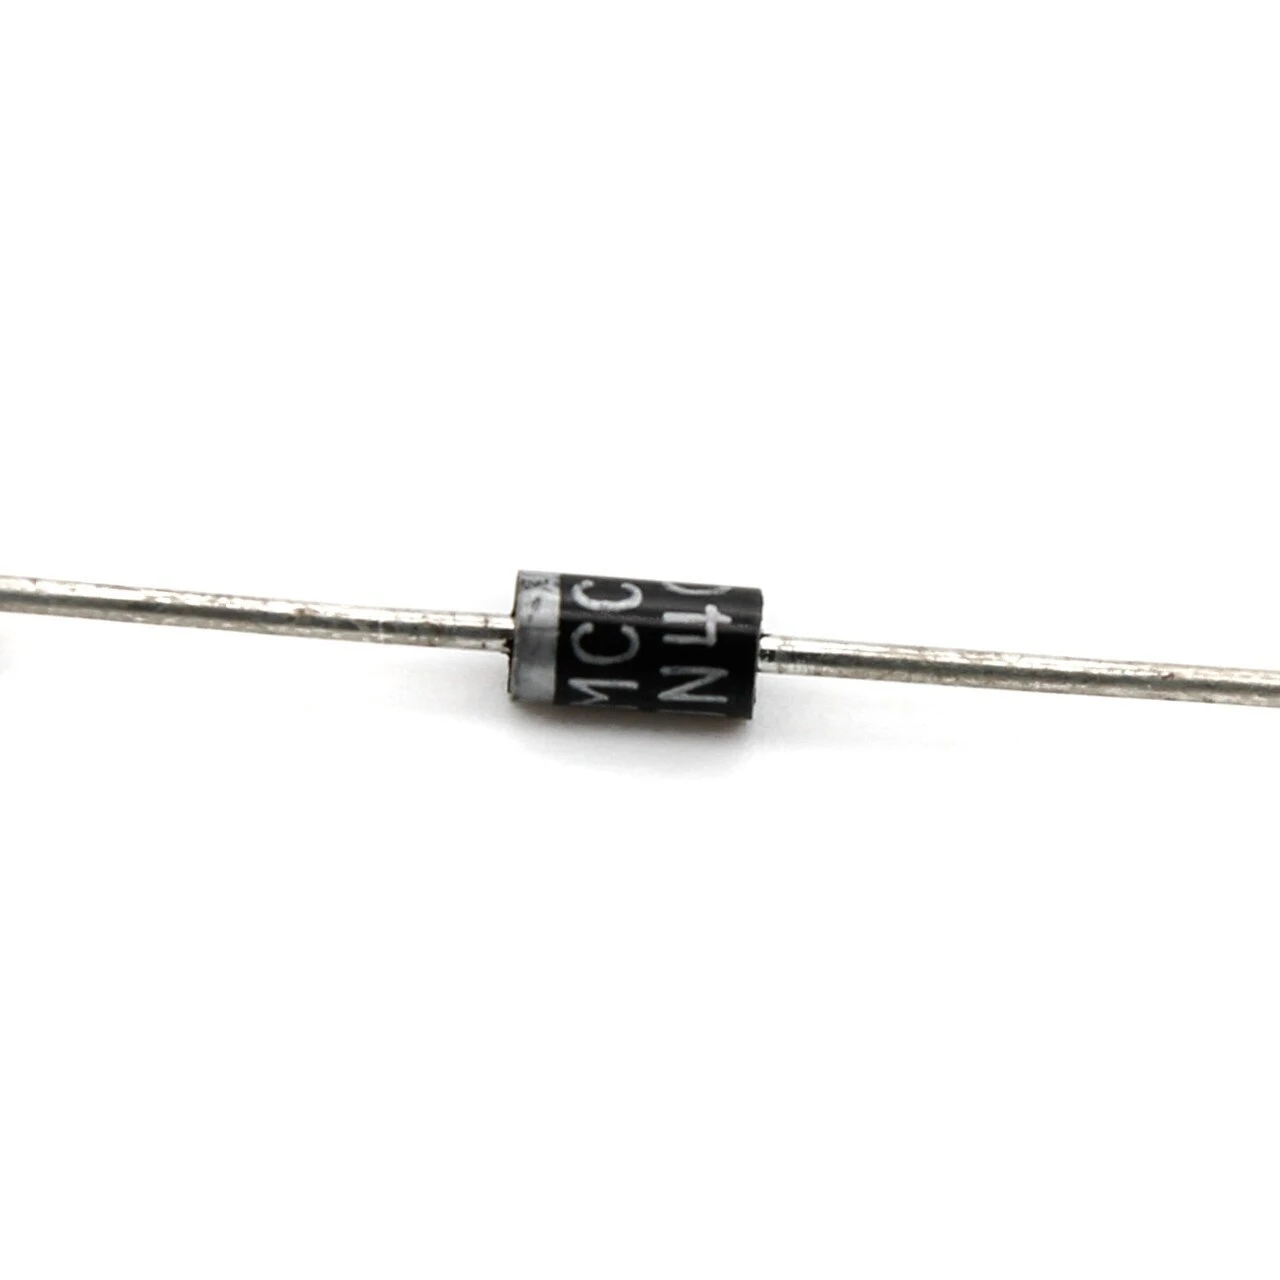
\includegraphics[width= 0.7\linewidth, height=0.7\textheight, keepaspectratio]{1n4004}
				\vspace{0.5cm}
			\caption{Diode 1N4004}
		\end{subfigure}
		\hfill
		\begin{subfigure}[b]{0.30\textwidth}
			\centering
		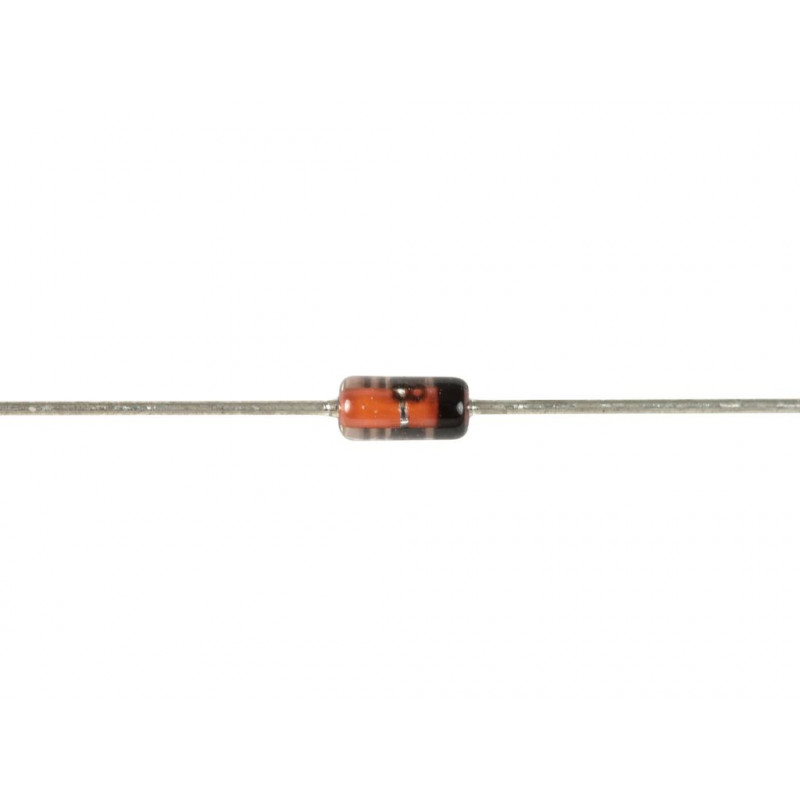
\includegraphics[width= 0.7\linewidth, height=0.7\textheight, keepaspectratio]{1n4148}
				\vspace{0.5cm}	
			\caption{Diode 1N4148}
		\end{subfigure}
		\hfill
		\begin{subfigure}[b]{0.30\textwidth}
			\centering
			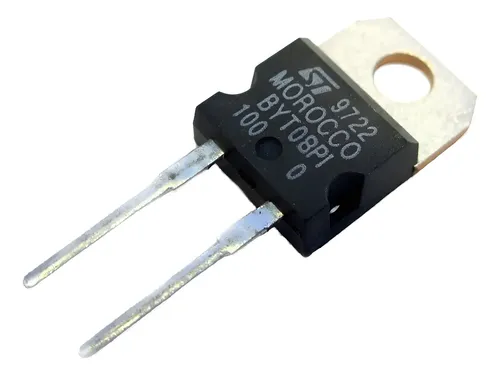
\includegraphics[width= 0.7\linewidth, height=0.7\textheight, keepaspectratio]{byt08}
				\vspace{0.5cm}
			\caption{Diode roue libre BYT08P}
		\end{subfigure}
		\caption{Diodes utilis\'ees dans le circuit}
		\label{fig:diodes}
	\end{figure}
	
	%%=========================================================
	\chapter{\'Etude Th\'eorique}
	
	Le circuit est segment\'e en deux parties~: la \textbf{partie commande}
	et la \textbf{partie puissance}.
	
	\section{Partie Commande}
	
	\subsection{Bloc d'Alimentation}

		L'alimentation est r\'ealis\'ee \`a partir d'un transformateur secteur
		220\,V/2$\times$12\,V/12\,VA. Un pont de diodes 1N4004 assure le
		redressement double alternance. Deux condensateurs de filtrage
		(C5, C6 = 2200\,$\mu$F) lissent la tension redress\'ee. Les r\'egulateurs
		7812 et 7912 fournissent $+12$\,V et $-12$\,V stabilis\'es. Le LM317T
		d\'elivre une tension ajustable pour le circuit de r\'ef\'erence.
	
	
	\begin{figure}[H]
		\centering
		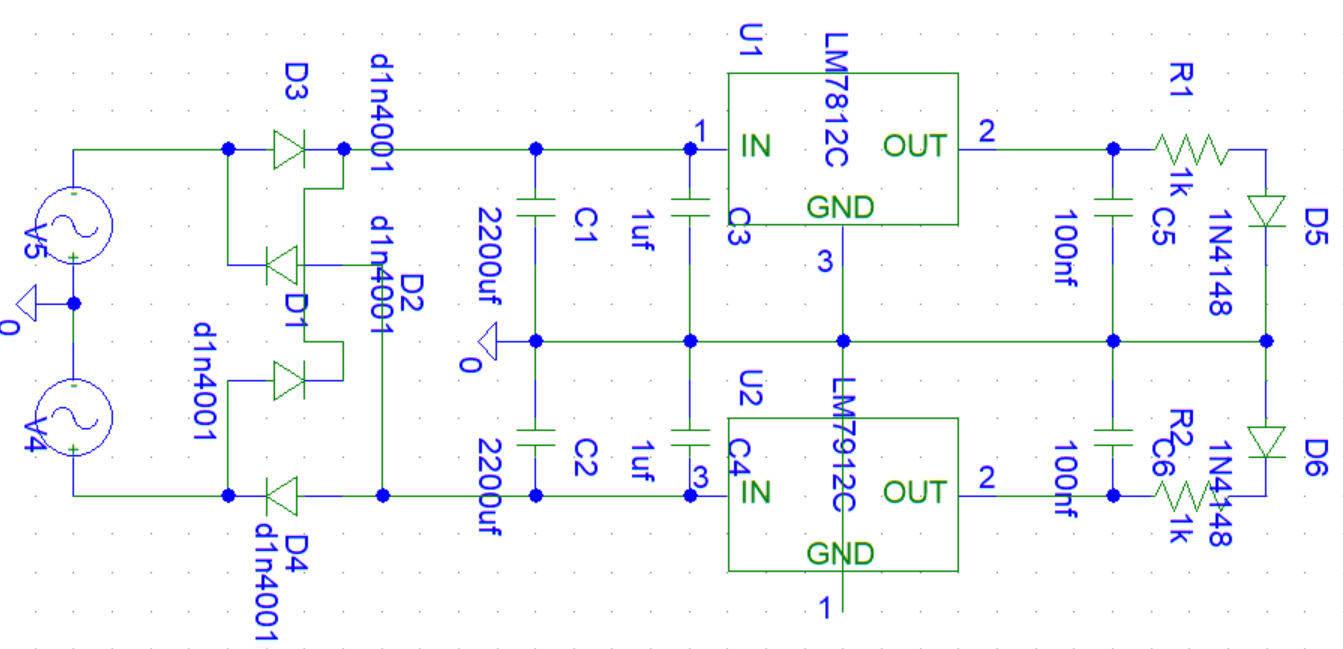
\includegraphics[width=\linewidth, height=\textheight, keepaspectratio]{bloc_alim}
				\vspace{1.5cm}
		\caption{Sch\'ema du bloc d'alimentation (PSpice)}
		\label{fig:alim_schema}
	\end{figure}
	

	
	\subsubsection{Redressement}

	
		Le pont de diodes 1N4004 convertit la tension AC en DC. Pendant chaque
		demi-alternance, deux diodes conductrices assurent un courant
		unidirectionnel \`a travers la charge.
		
	\begin{figure}[H]
		\centering
		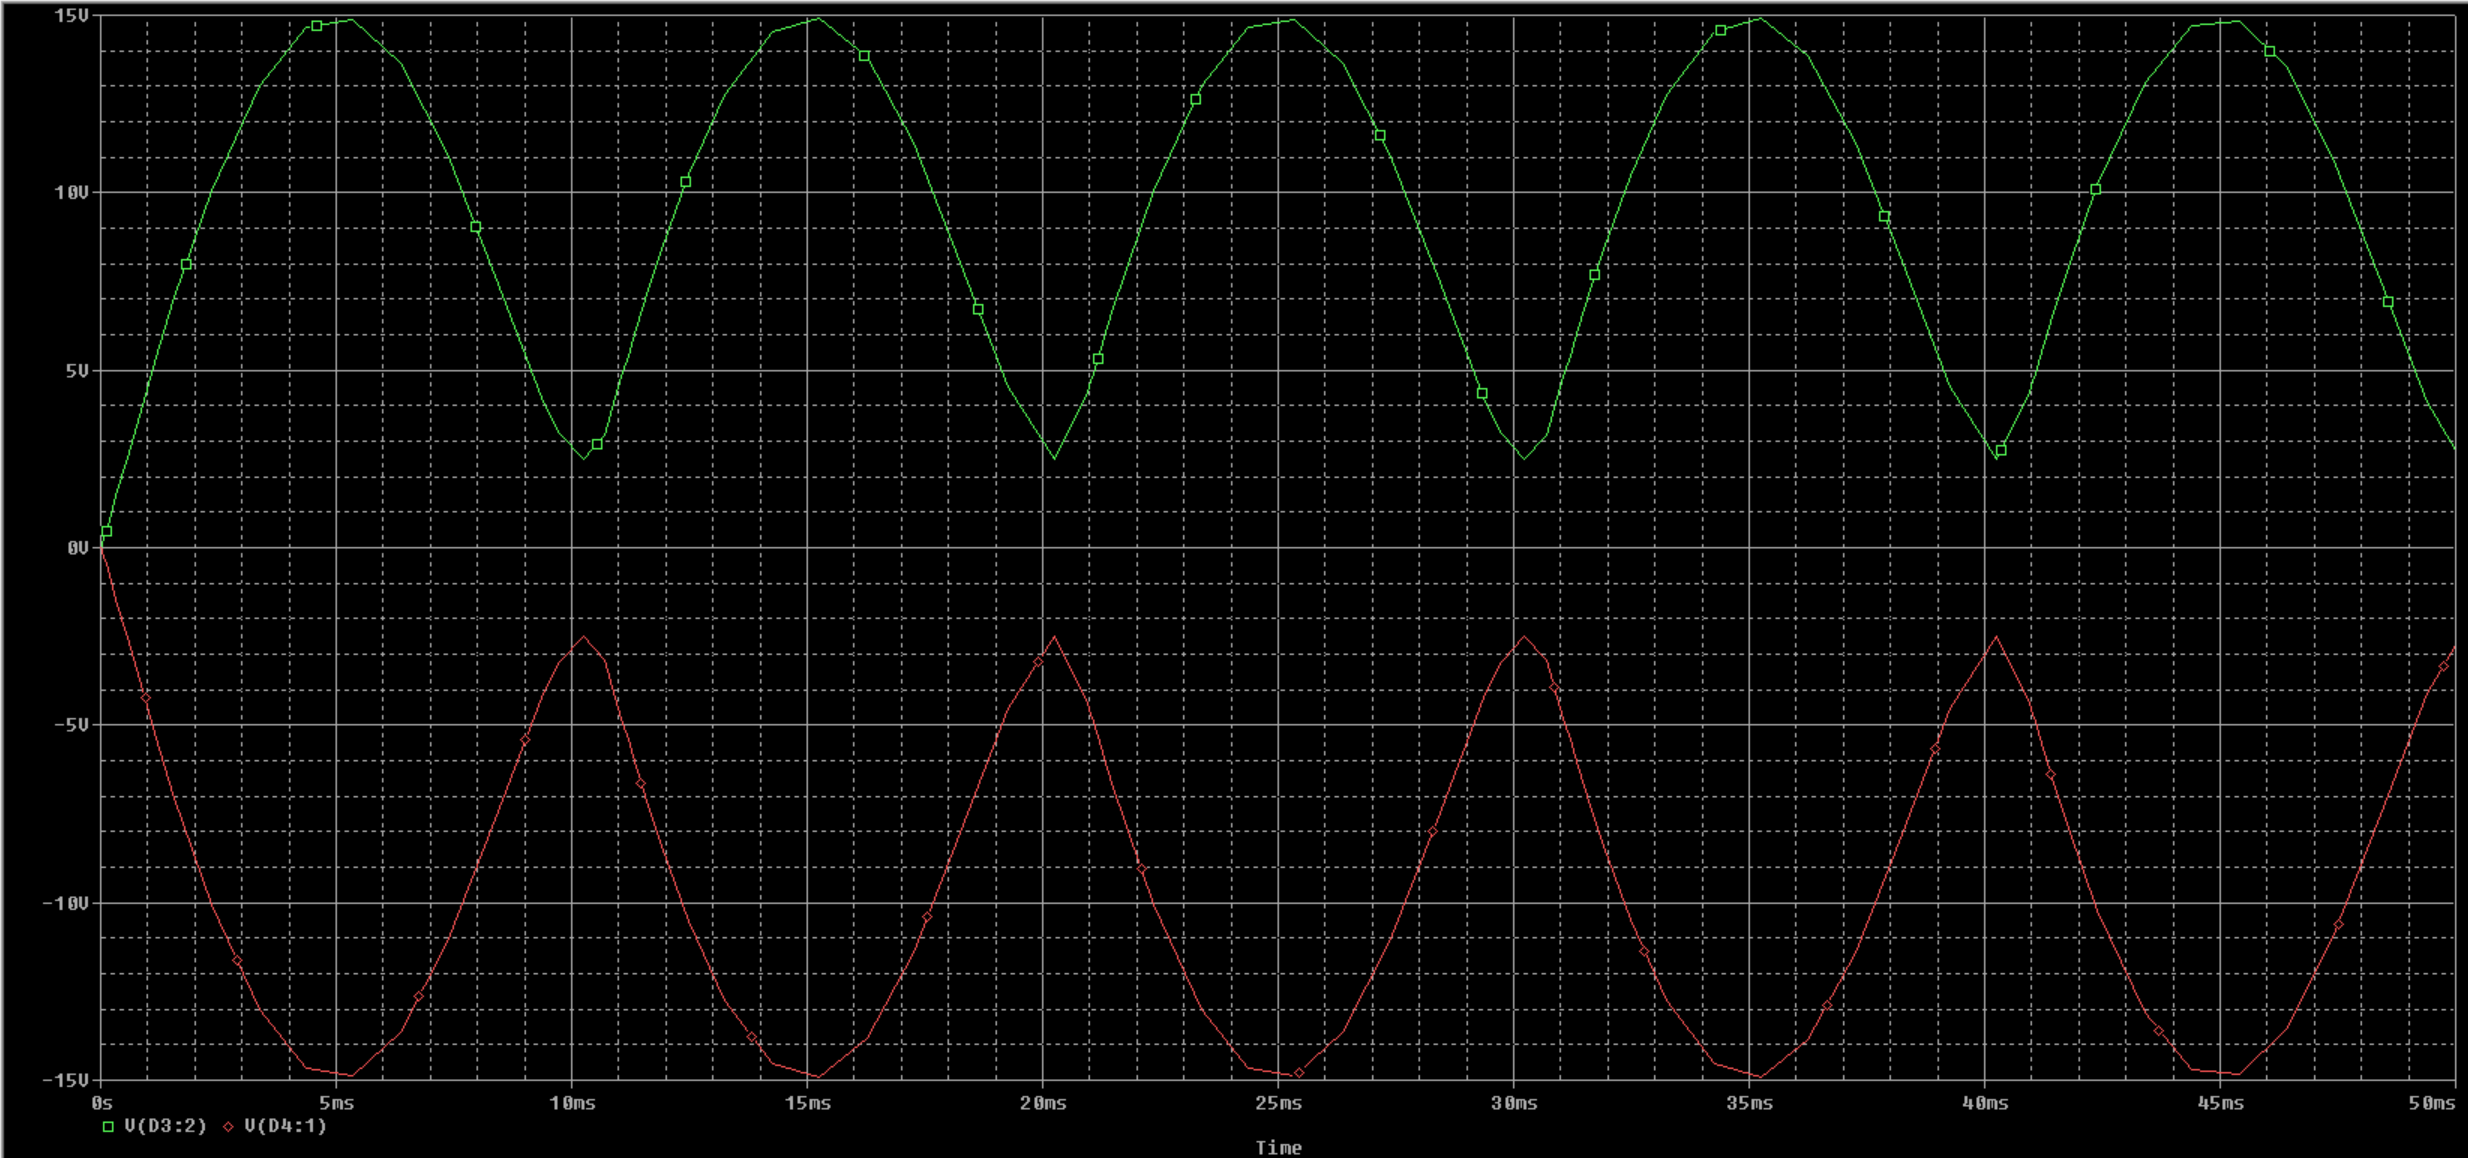
\includegraphics[width=\linewidth, height=0.3\textheight, keepaspectratio]{sim_red}
		\vspace{0.5cm}
		\caption{Signal de sortie du pont de diodes (simulation PSpice)}
		\label{fig:red_sim}
	\end{figure}

	\subsubsection{Filtrage et R\'egulation}

		Les condensateurs C5 et C6 (2200\,$\mu$F) lissent les ondulations.
		Les r\'egulateurs 7812 et 7912 maintiennent des tensions stabilis\'ees
		de $\pm12$\,V ind\'ependamment des variations de charge.
		
	\begin{figure}[H]
		\centering
		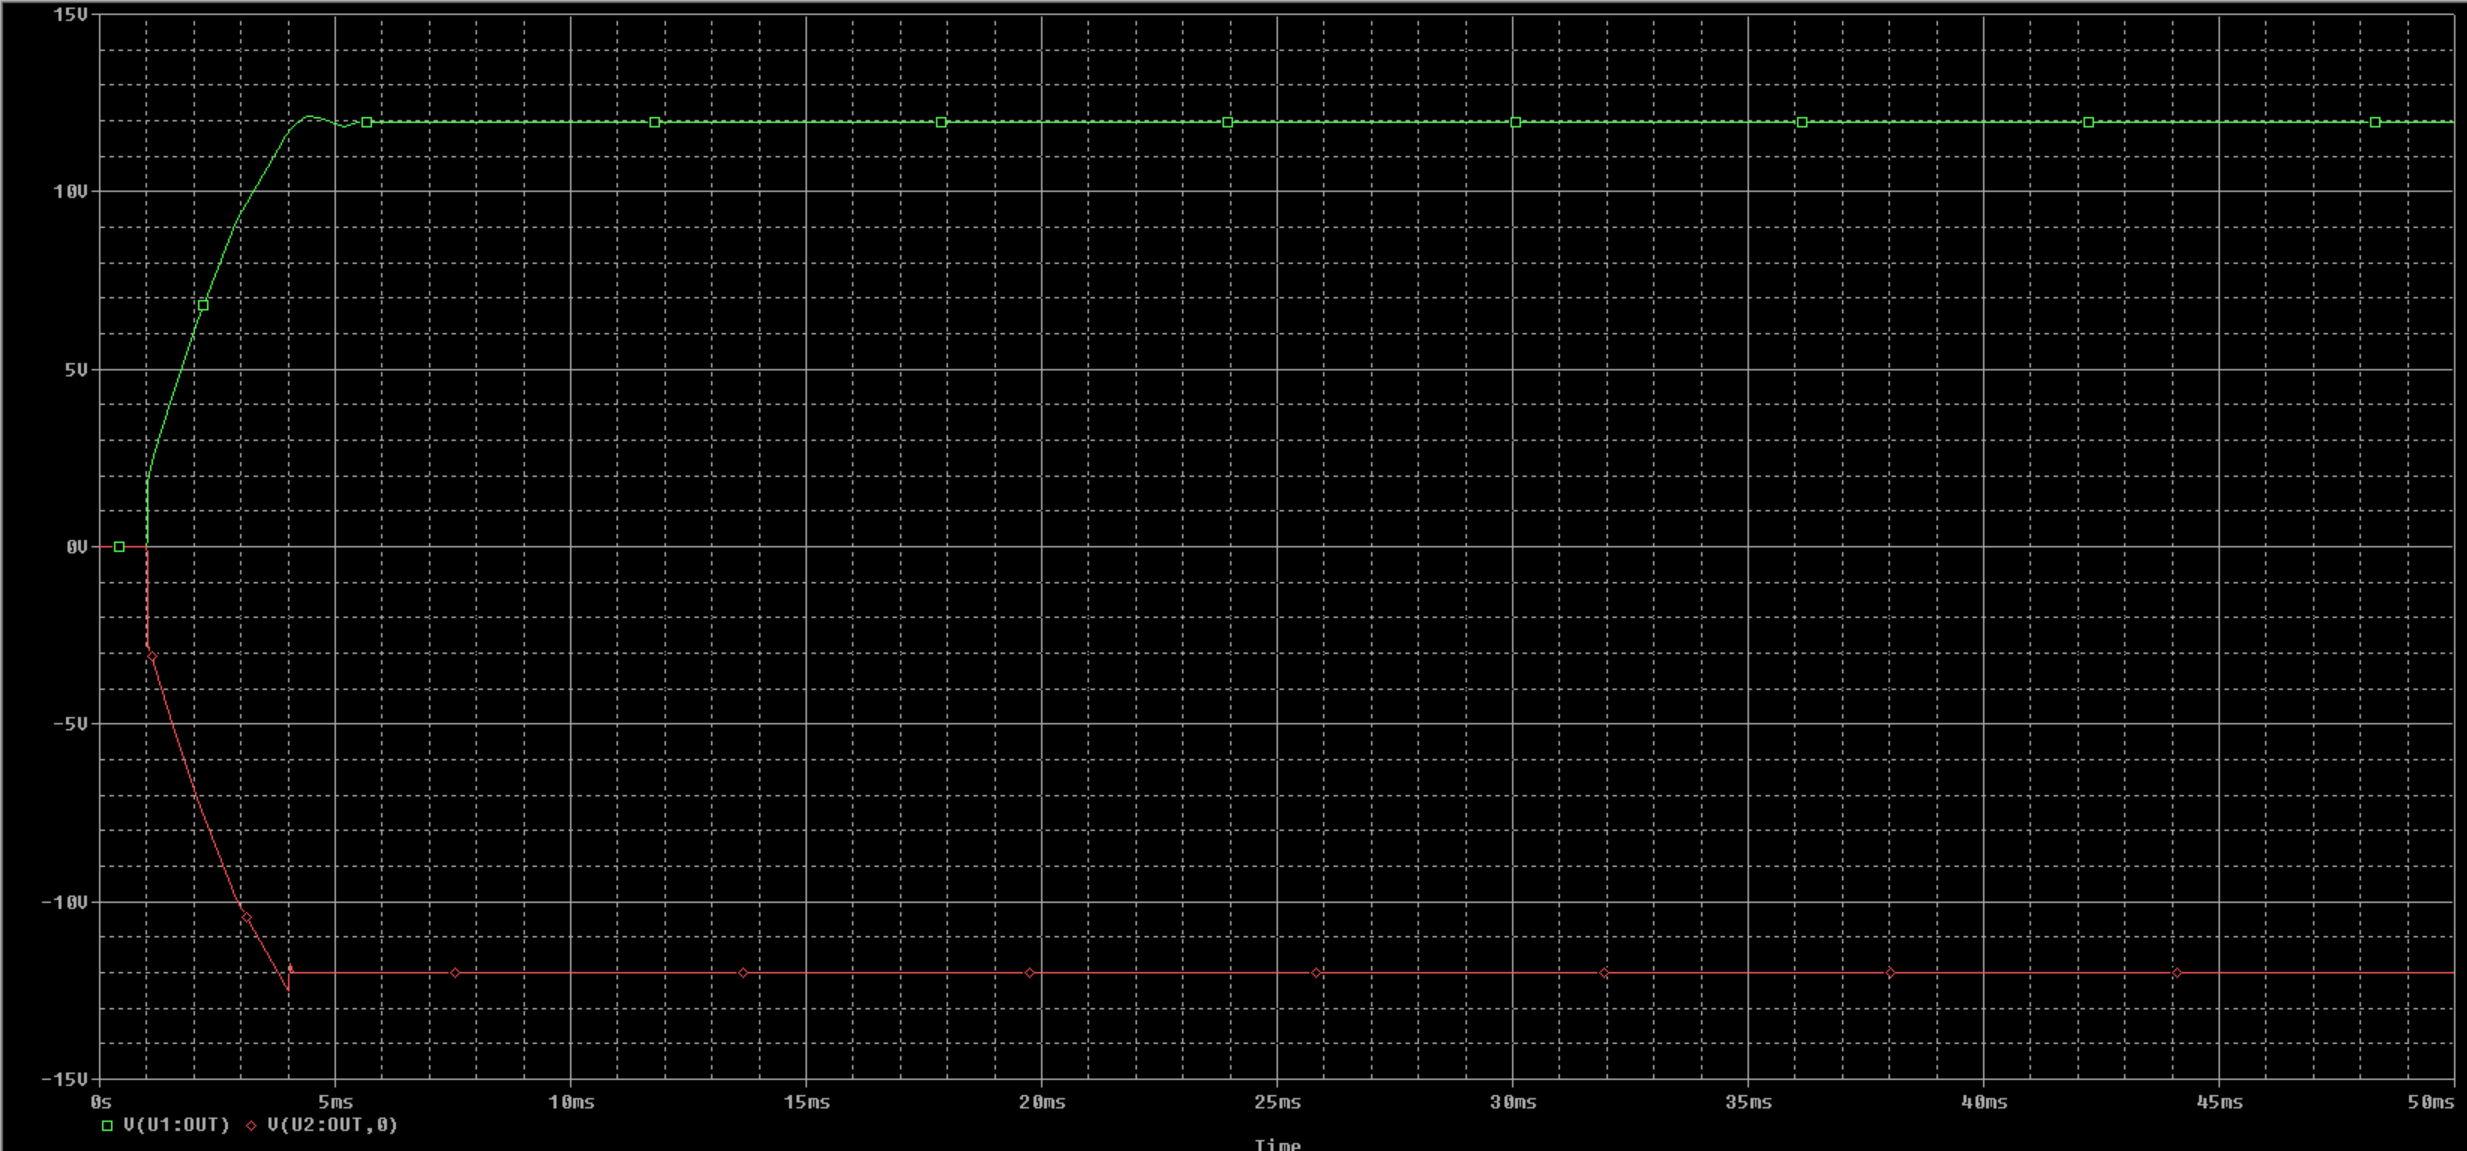
\includegraphics[width=\linewidth, height=0.3\textheight, keepaspectratio]{sim_reg}
		\vspace{0.5cm}
		\caption{Signal de sortie du bloc d'alimentation (simulation PSpice)}
		\label{fig:alim_signal}
	\end{figure}
	
	%%----------------------------------------------------------
	\subsection{Bloc G\'en\'eration MLI}
	
	Le c\oe ur de la g\'en\'eration du signal PWM est le \textbf{NE555N} (IC3)
	mont\'e en mode astable. La tension moyenne $V_{moy}$ appliqu\'ee au moteur
	est~:
	\begin{equation}
		V_{moy} = \alpha \cdot V_{cc}, \qquad \alpha = \frac{t_{on}}{T}
	\end{equation}
	
	En variant le potentiom\`etre P1 (10\,k$\Omega$), le rapport cyclique
	$\alpha$ varie, modifiant directement la vitesse du moteur.
	
	\begin{figure}[H]
		\centering
		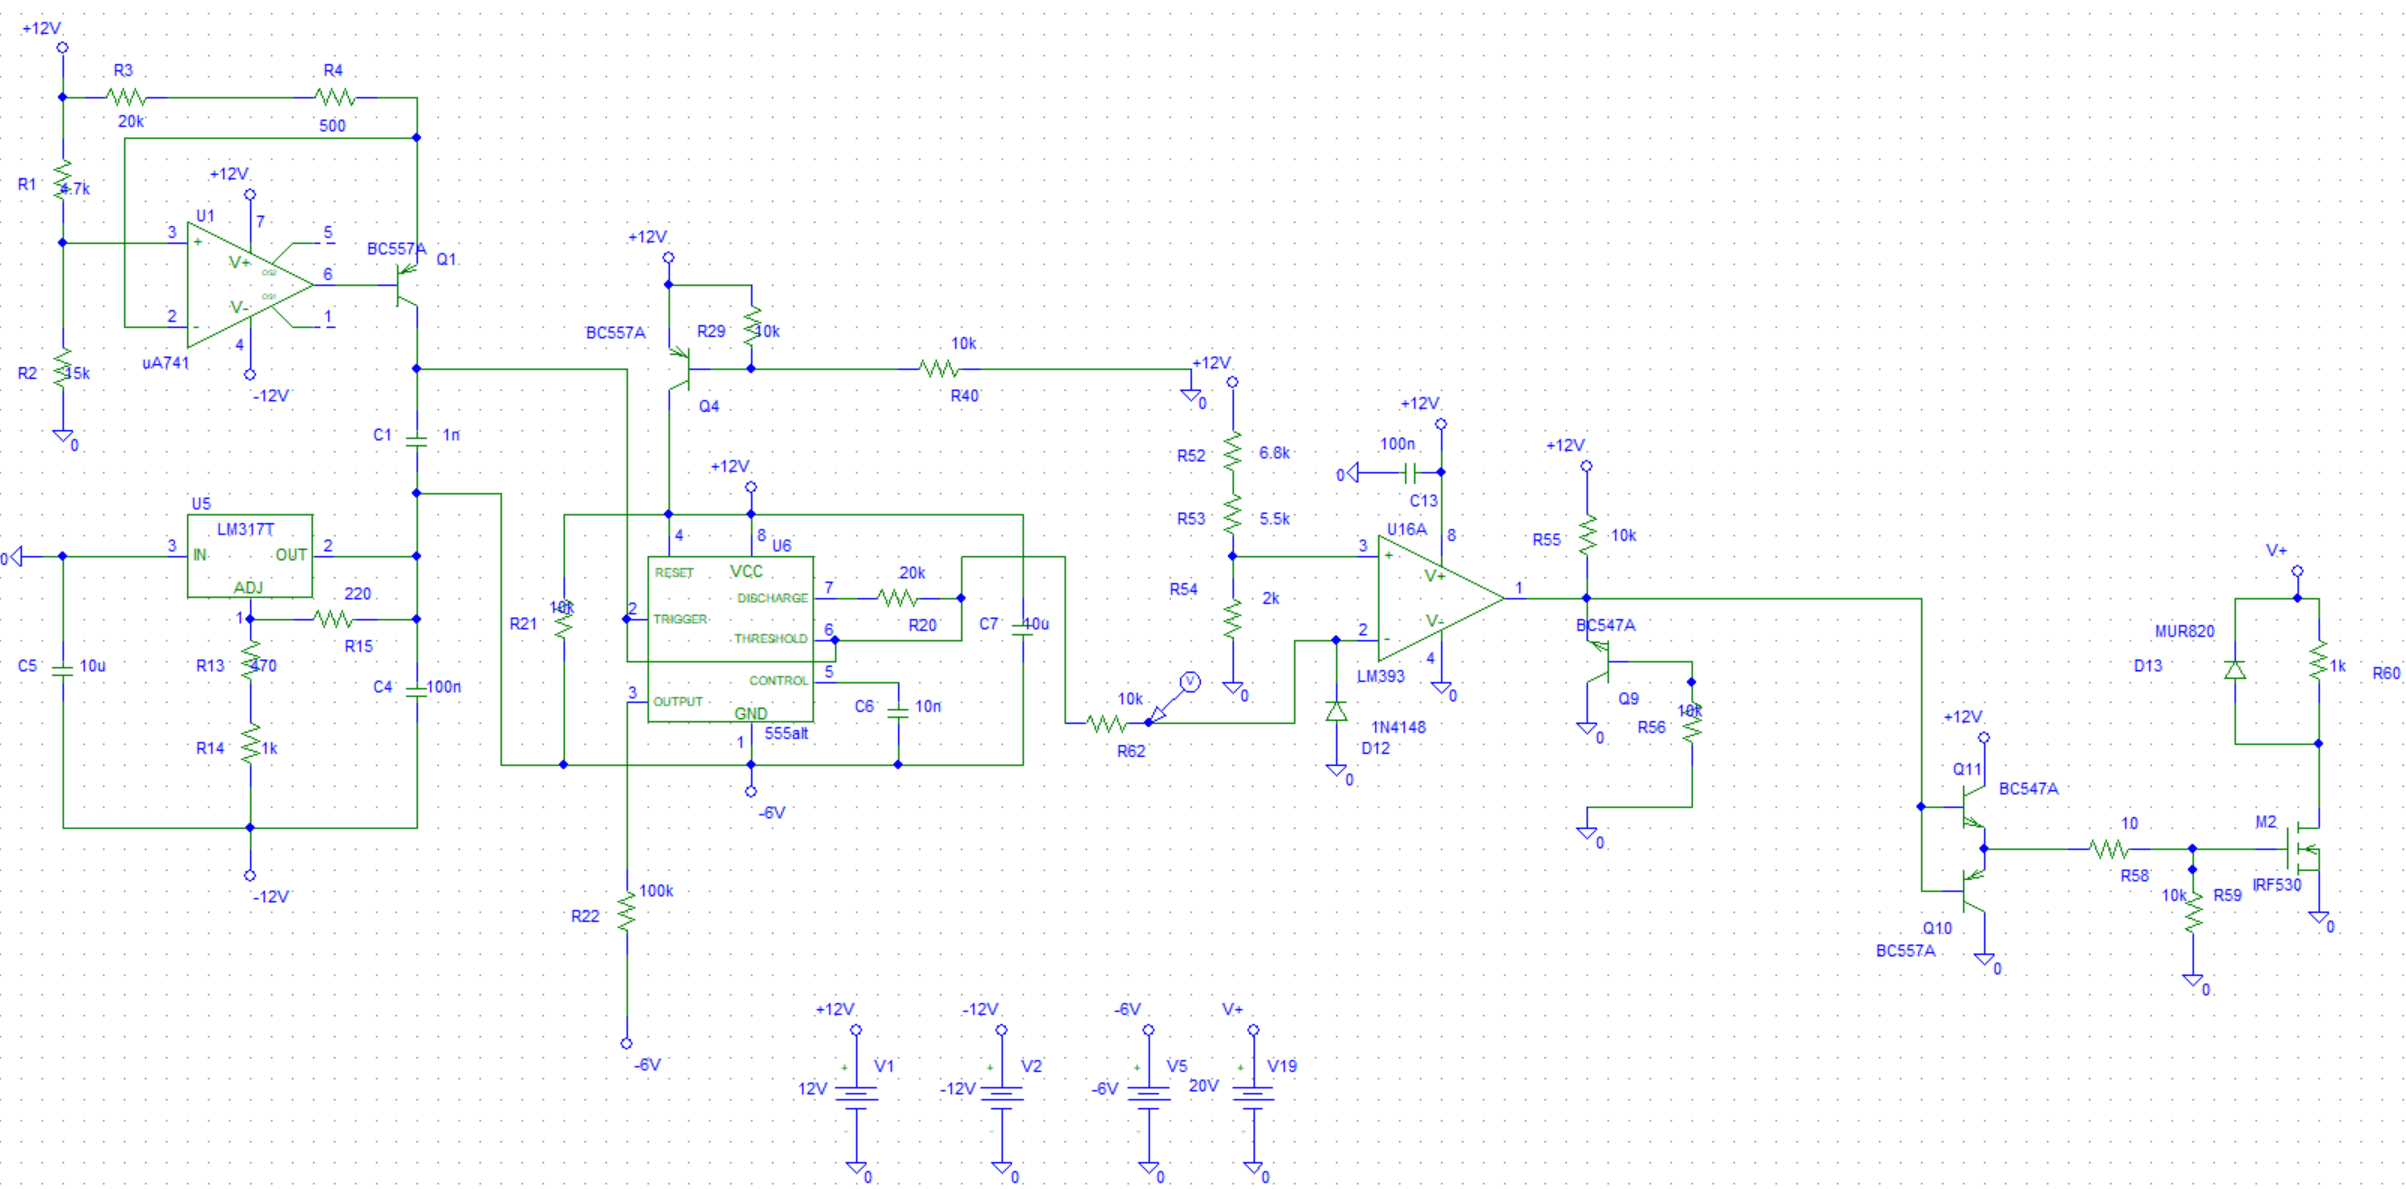
\includegraphics[width=1.1\linewidth, height=1.7\textheight, keepaspectratio]{sch_mli}
			\vspace{0.5cm}
		\caption{Sch\'ema du bloc MLI}
		\label{fig:mli_schema}
	\end{figure}
		
		
	\subsubsection{G\'en\'eration du signal dents de scie}
	
	Le NE555N est configur\'e en mode astable. Les diodes D5 et D6 (1N4148)
	orientent s\'epar\'ement les courants de charge et de d\'echarge du
	condensateur C4 (10\,nF), produisant une rampe quasi-lin\'eaire.
	
	\begin{figure}[H]
		\centering
		\begin{subfigure}[b]{\textwidth}
			\centering
			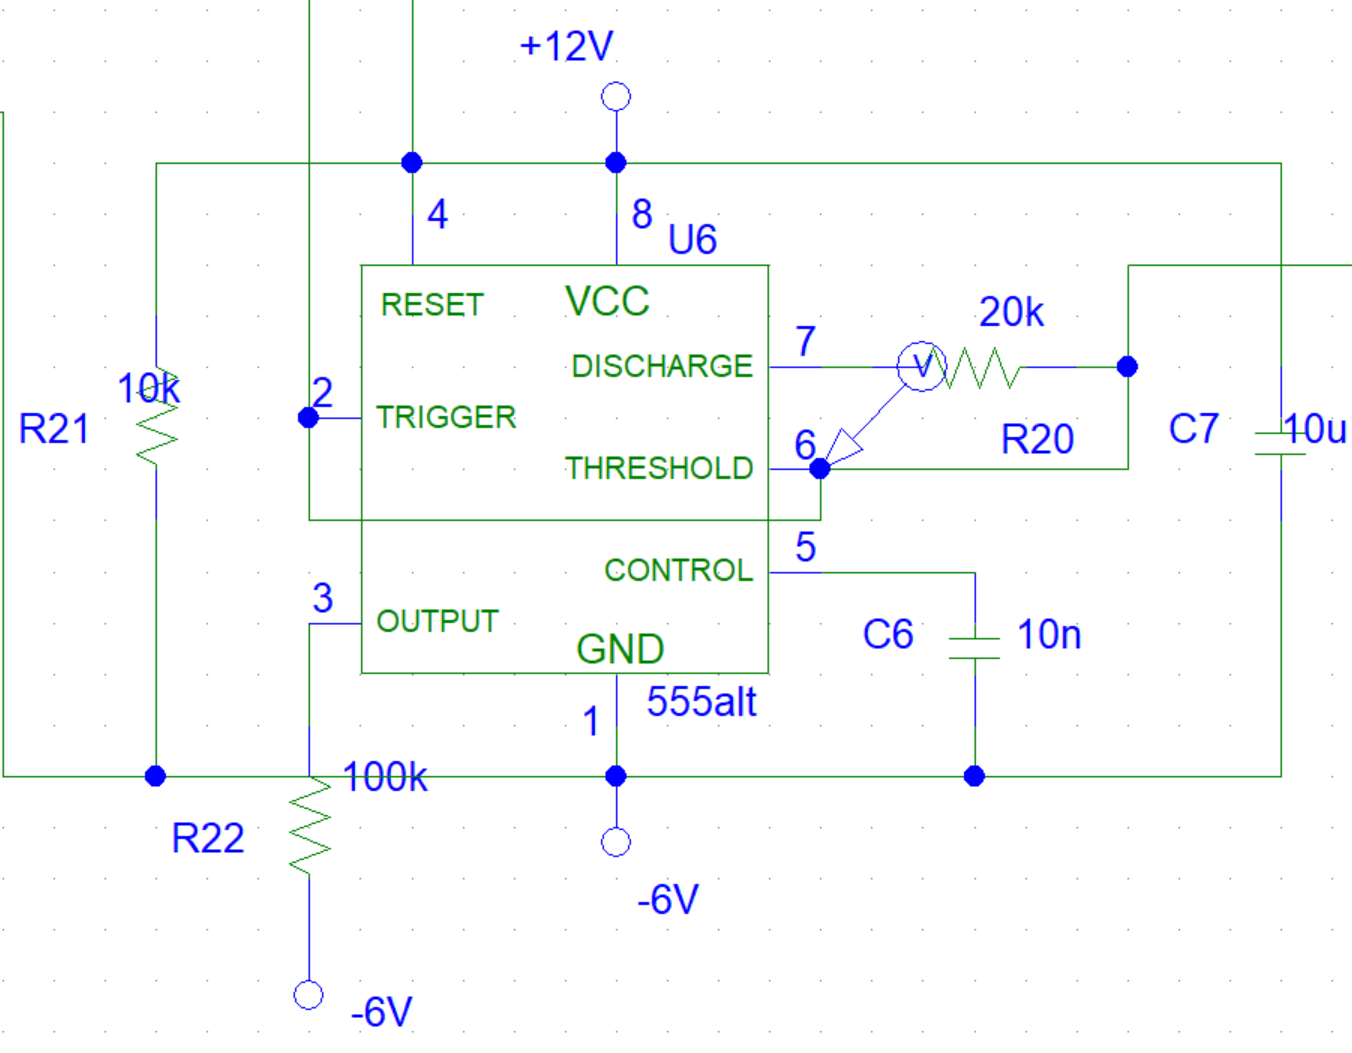
\includegraphics[width=\linewidth, height=0.35\textheight, keepaspectratio]{sch_dent}
			\caption{Sch\'ema g\'en\'erateur (PSpice)}
		\end{subfigure}
		
		\vspace{0.4cm}
		
		\begin{subfigure}[b]{\textwidth}
			\centering
			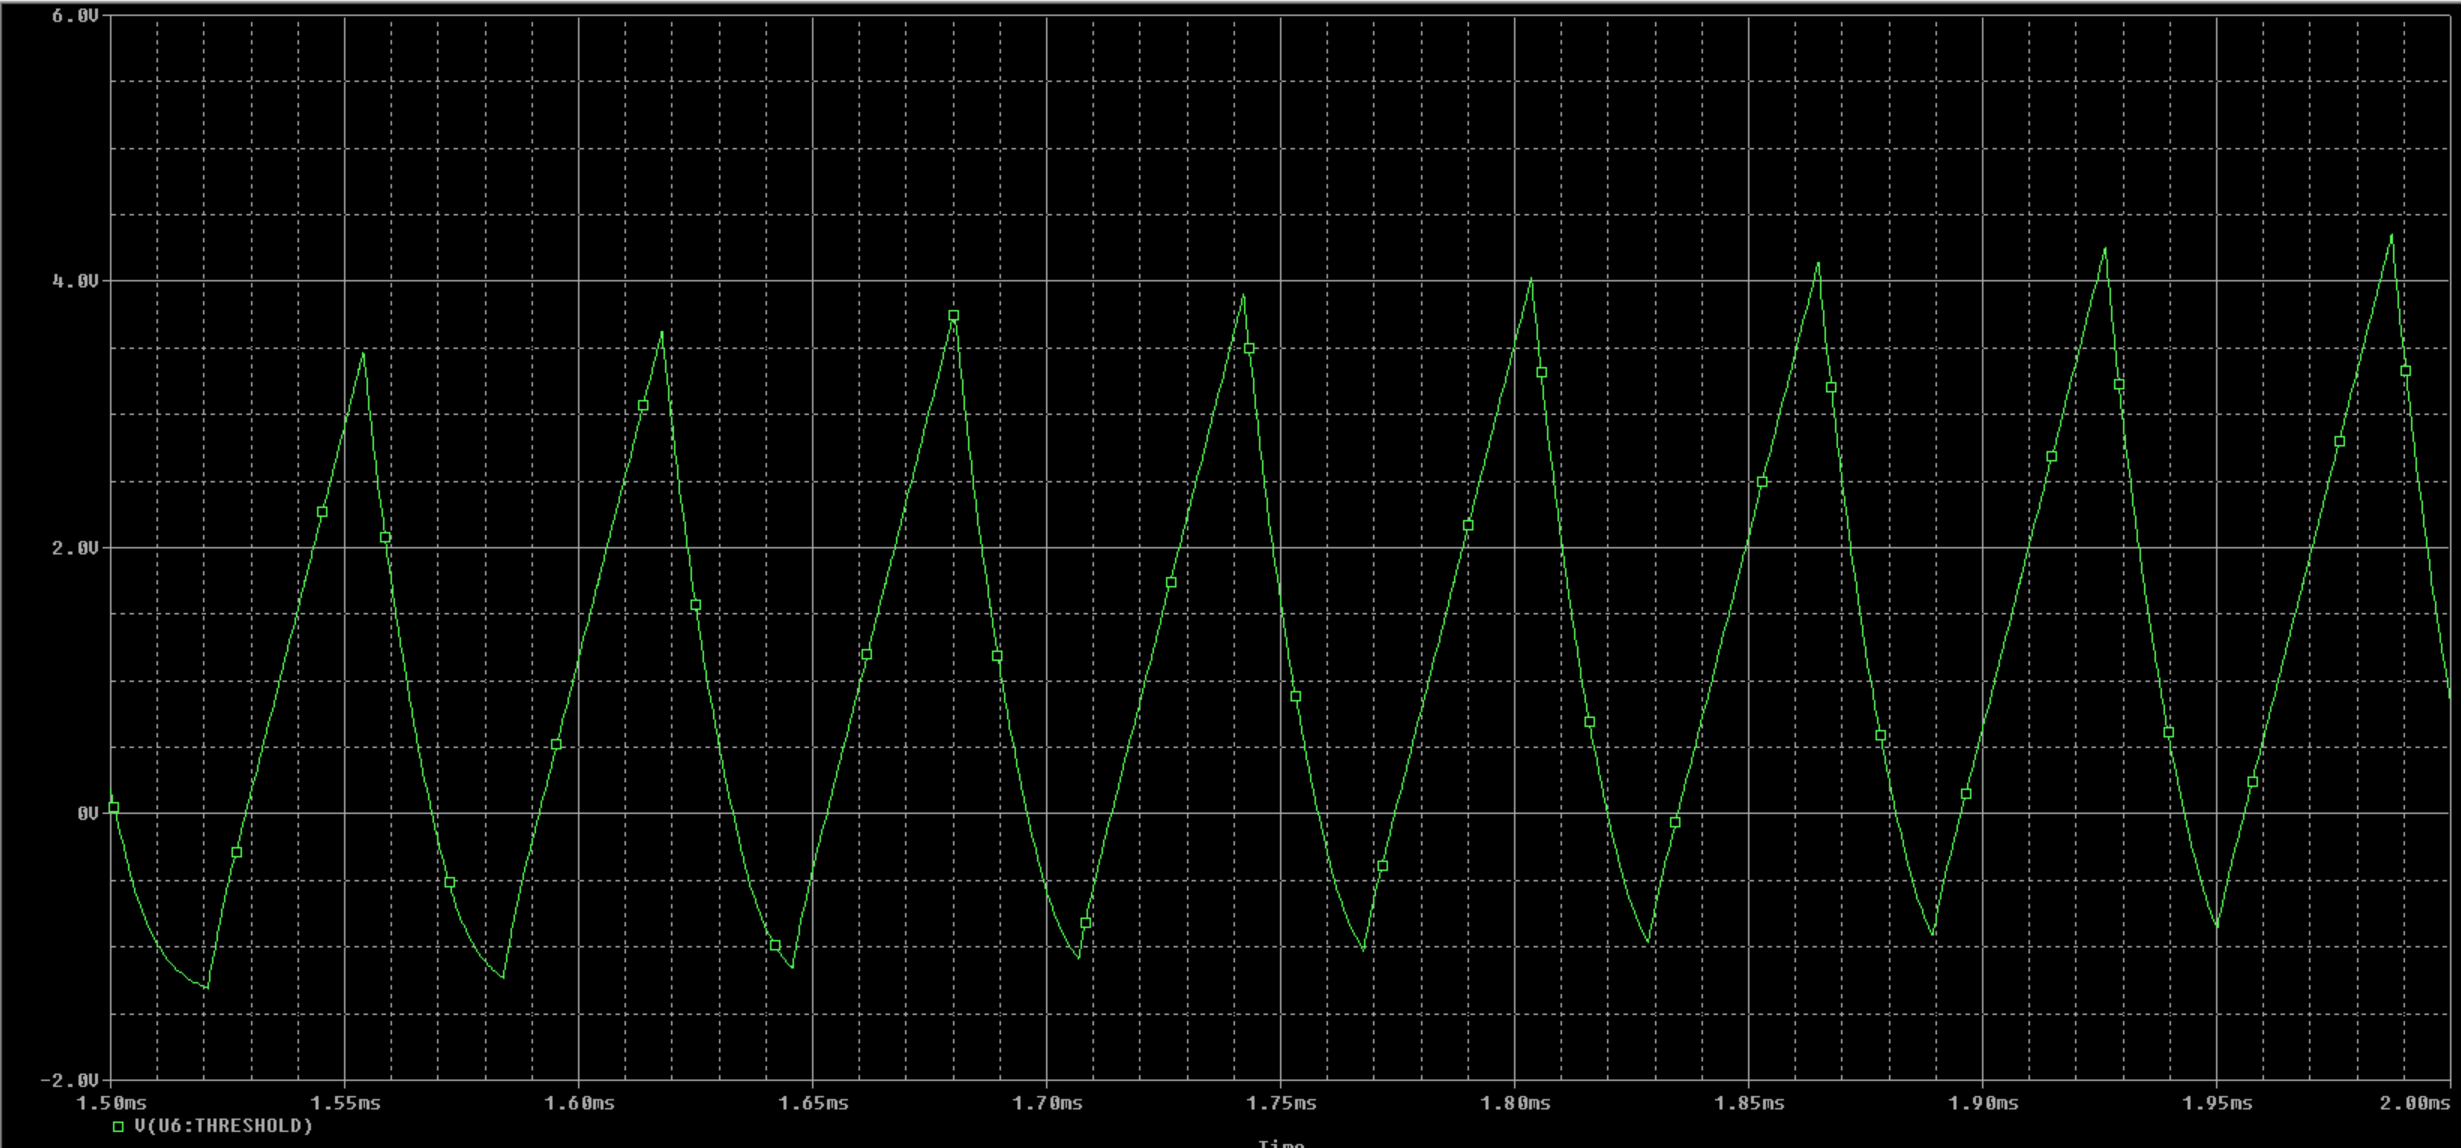
\includegraphics[width=\linewidth, height=0.35\textheight, keepaspectratio]{sim_dent}
			\caption{Signal dents de scie obtenu}
		\end{subfigure}
		\caption{G\'en\'eration du signal dents de scie avec le NE555N}
		\label{fig:dents_scie}
	\end{figure}

	
	\subsubsection{G\'en\'eration du signal MLI}
	
	Le signal MLI est obtenu en comparant le signal dents de scie avec la
	tension de r\'ef\'erence fournie par le $\mu$A741P. Le comparateur LM393N
	(IC6) effectue cette comparaison~: quand la consigne d\'epasse la porteuse,
	la sortie est haute~; sinon elle est basse.
	\begin{figure}[H]
		\centering
		\begin{subfigure}[b]{\textwidth}
			\centering
			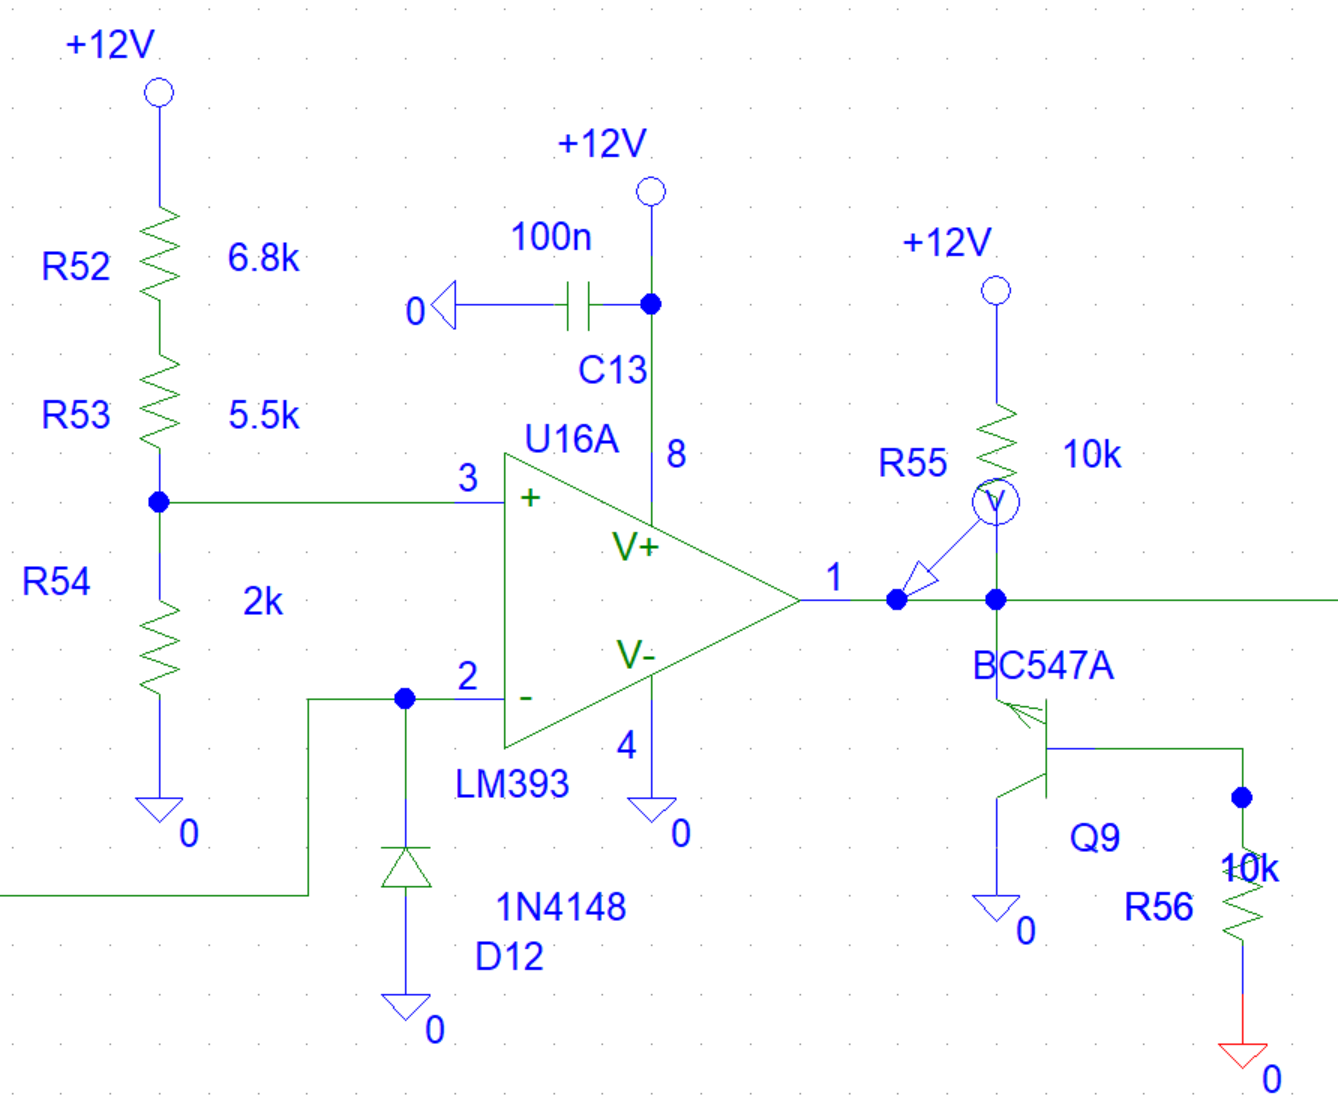
\includegraphics[width=\linewidth, height=0.35\textheight, keepaspectratio]{sch_mli1}
			\caption{Sch\'ema g\'en\'erateur MLI (PSpice)}
		\end{subfigure}
		
		\vspace{0.4cm}
		
		\begin{subfigure}[b]{\textwidth}
			\centering
			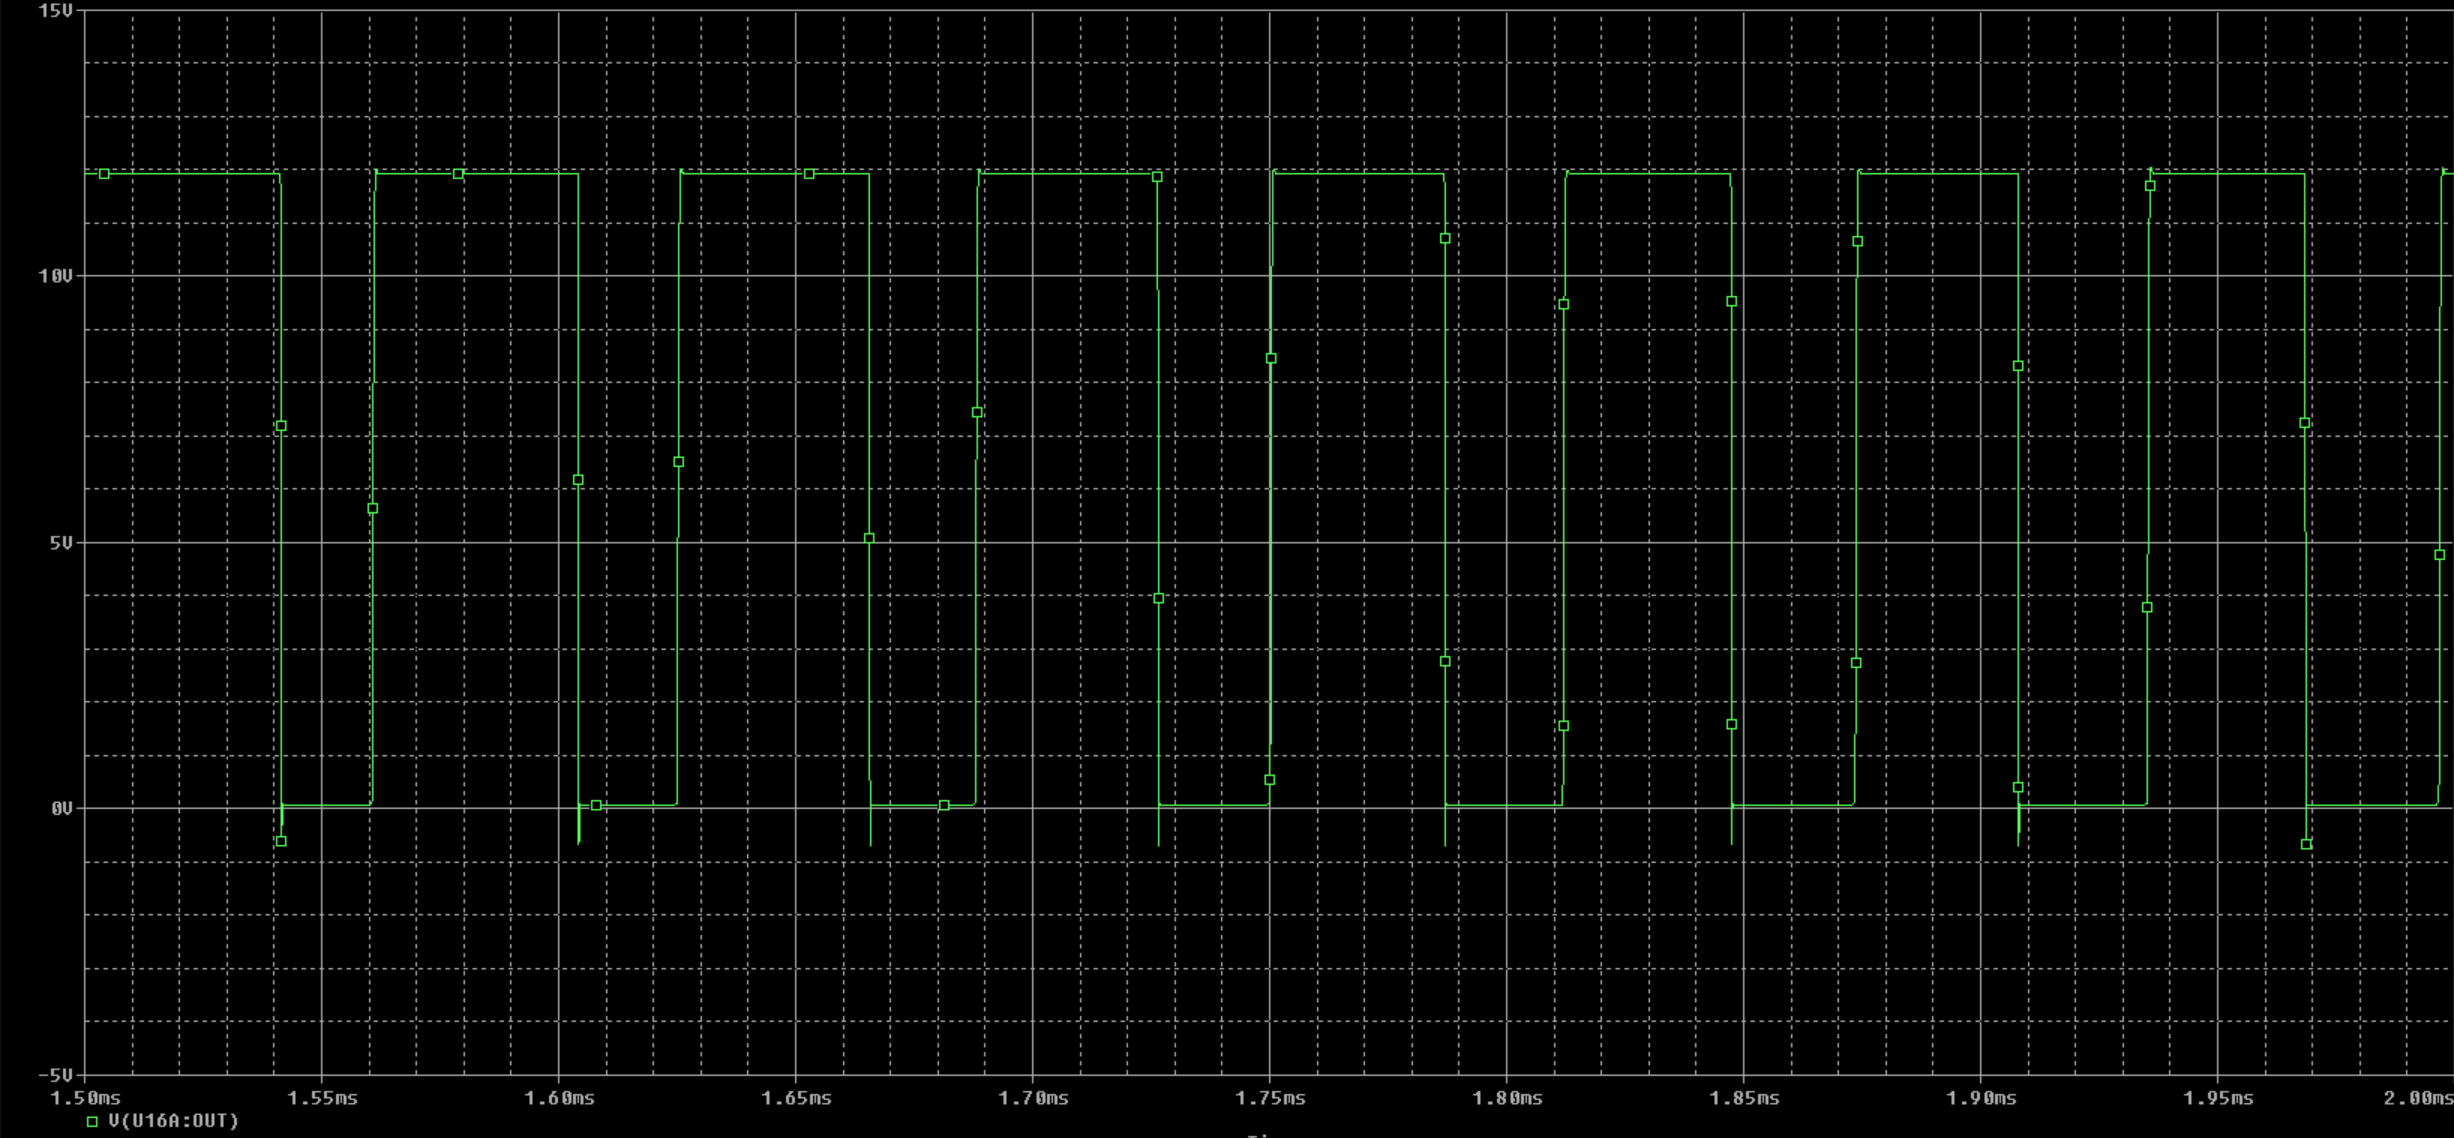
\includegraphics[width=\linewidth, height=0.35\textheight, keepaspectratio]{sim_mli}
			\caption{Signal MLI obtenu}
		\end{subfigure}
		\caption{G\'en\'eration du signal MLI par comparaison}
		\label{fig:mli}
	\end{figure}
	
	%%----------------------------------------------------------
	\subsection{Bloc Logique de Commande (CD4027N)}
	
	Deux bascules JK (IC7A et IC7B) assurent les fonctions marche/arr\^et et
	sens de rotation~:
	\begin{itemize}
		\item \textbf{IC7A~:} le bouton S1 fournit l'impulsion d'horloge~;
		la sortie Q d\'everrouille la cha\^ine de commande du MOSFET.
		\item \textbf{IC7B~:} le bouton S2 fait basculer Q, commandant le relais
		K1 via Q7 (2N2222), inversant la polarit\'e du moteur.
	\end{itemize}
	
	\begin{figure}[H]
		\centering
		\begin{subfigure}[b]{\textwidth}
			\centering
			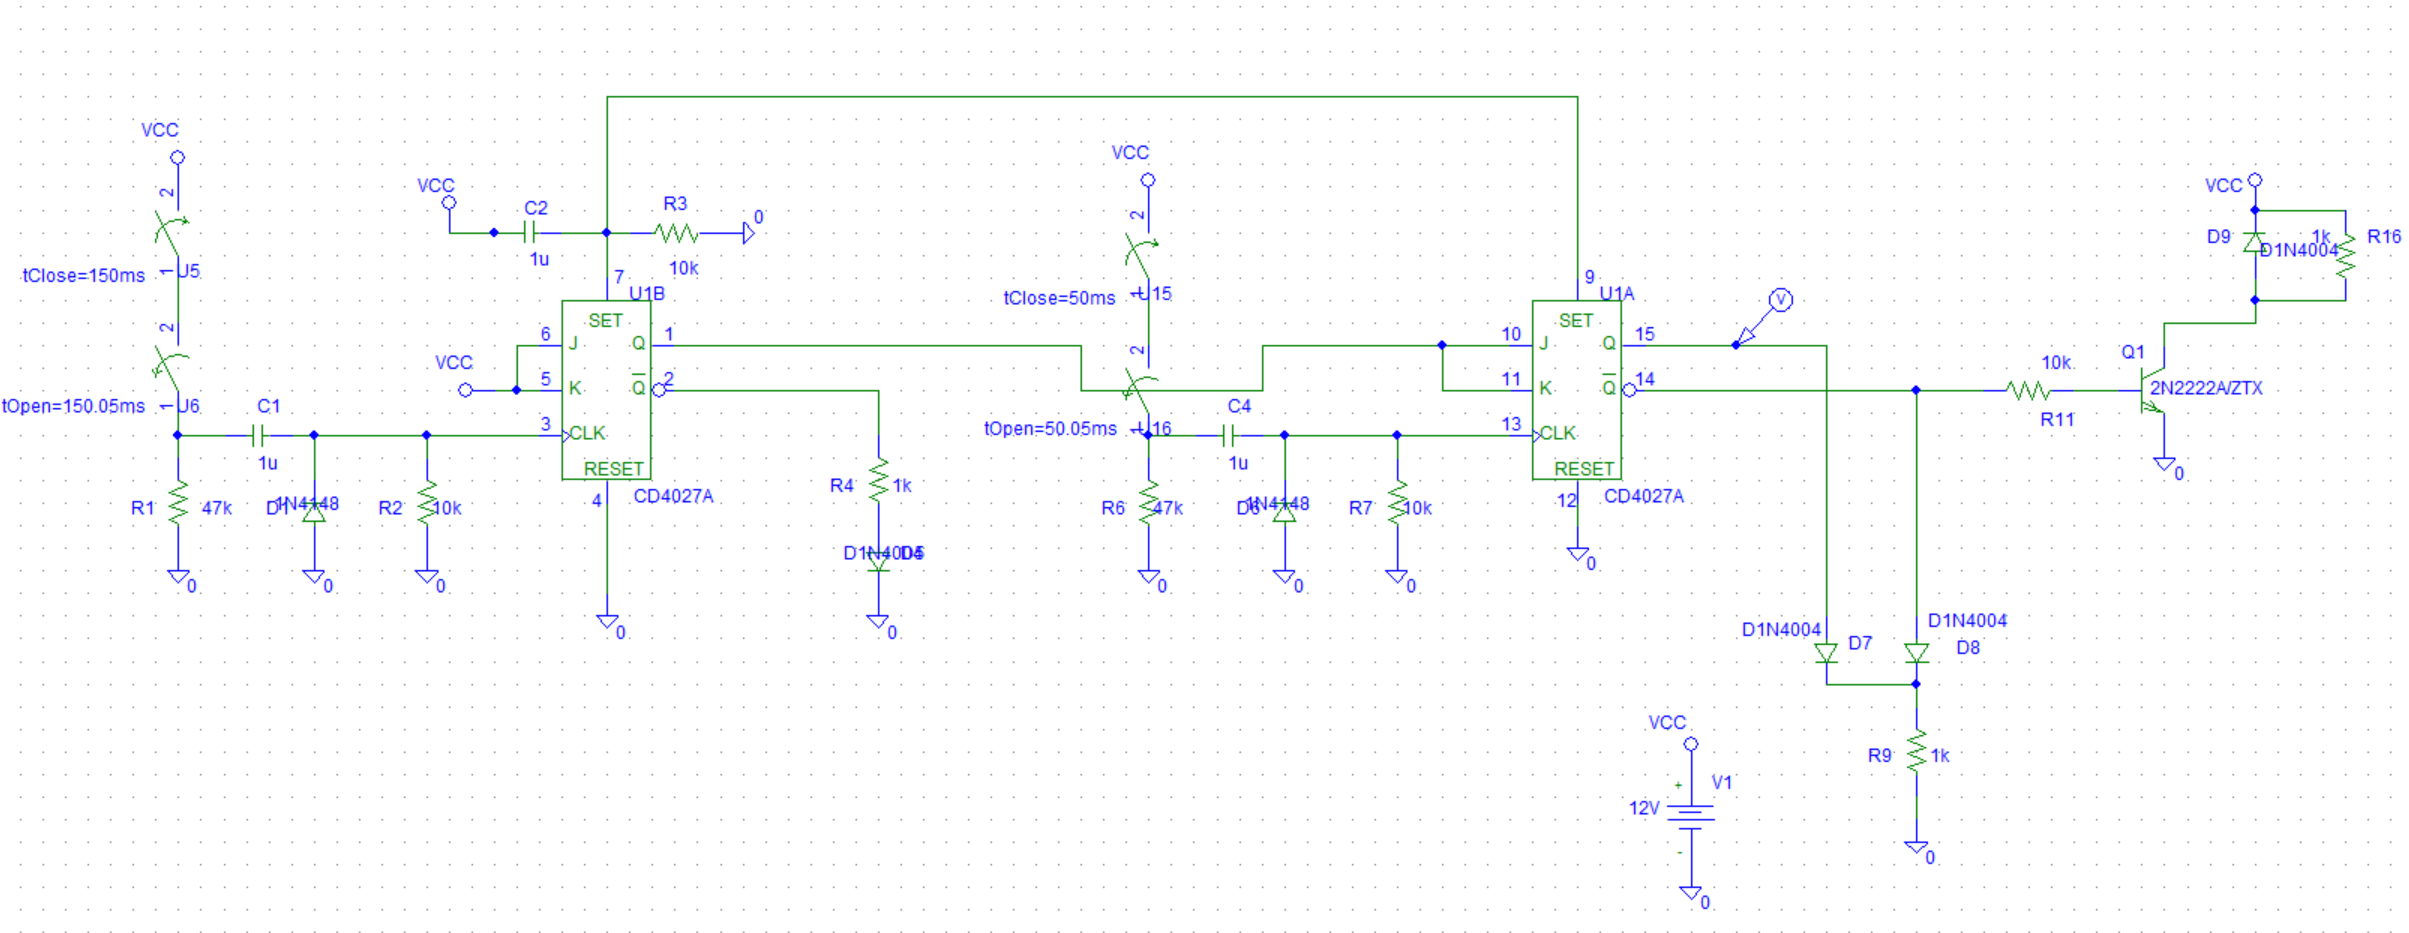
\includegraphics[width=\linewidth, height=0.35\textheight, keepaspectratio]{sch_commande}
			\caption{Sch\'ema de commande marche/arr\^et et sens de rotation (PSpice)}
		\end{subfigure}
		
		\vspace{0.4cm}
		
		\begin{subfigure}[b]{0.48\textwidth}
			\centering
			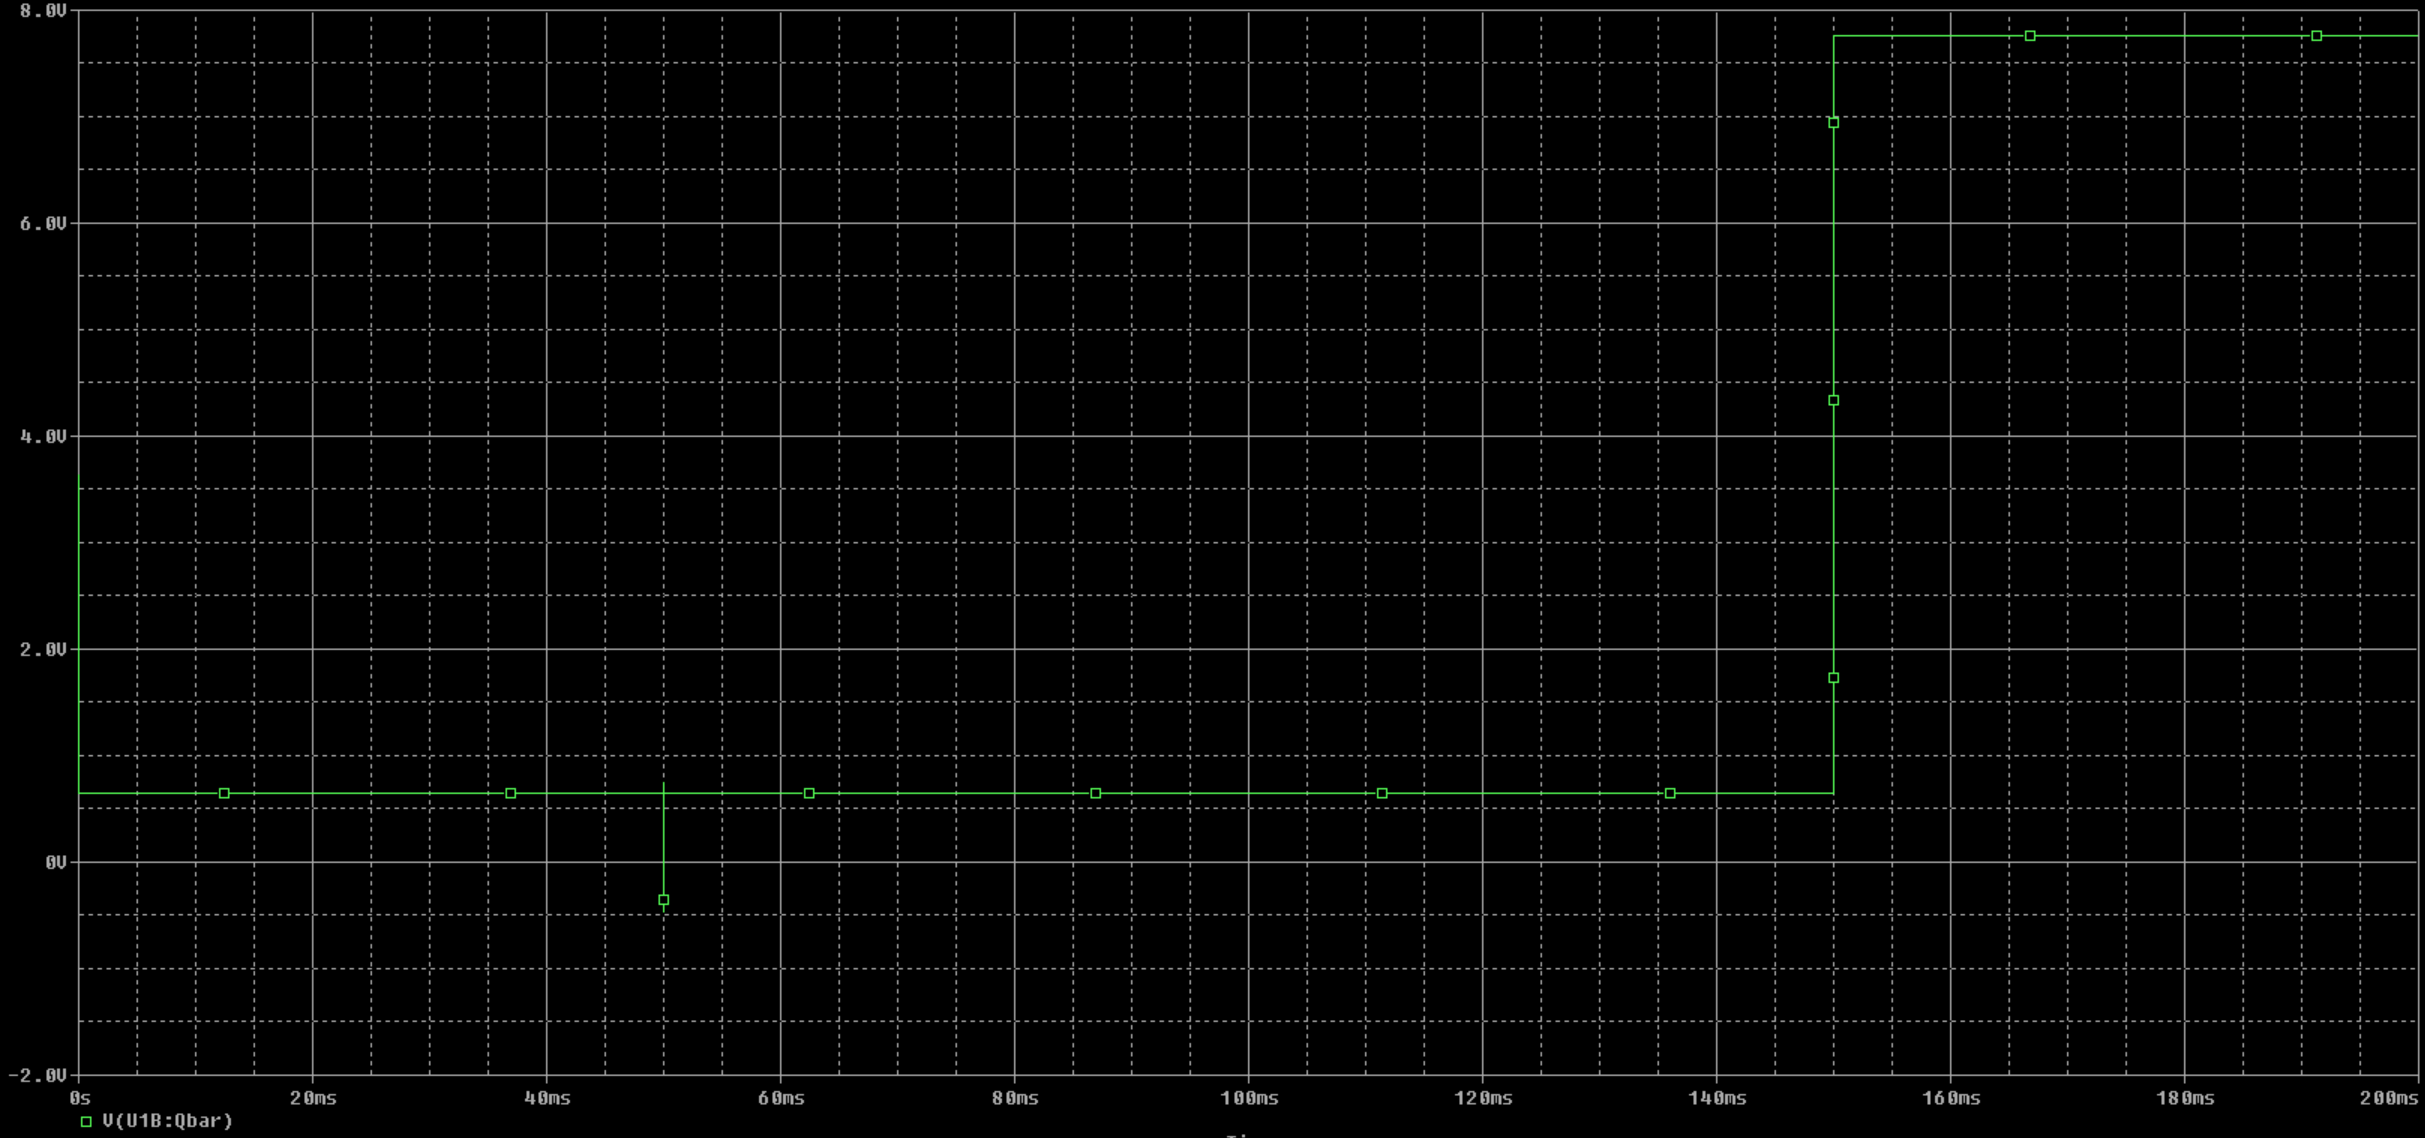
\includegraphics[width=\linewidth, height=0.30\textheight, keepaspectratio]{sim_marche}
			\caption{Simulation -- moteur en marche}
		\end{subfigure}
		
		\vspace{0.4cm}
		
		\begin{subfigure}[b]{0.48\textwidth}
			\centering
			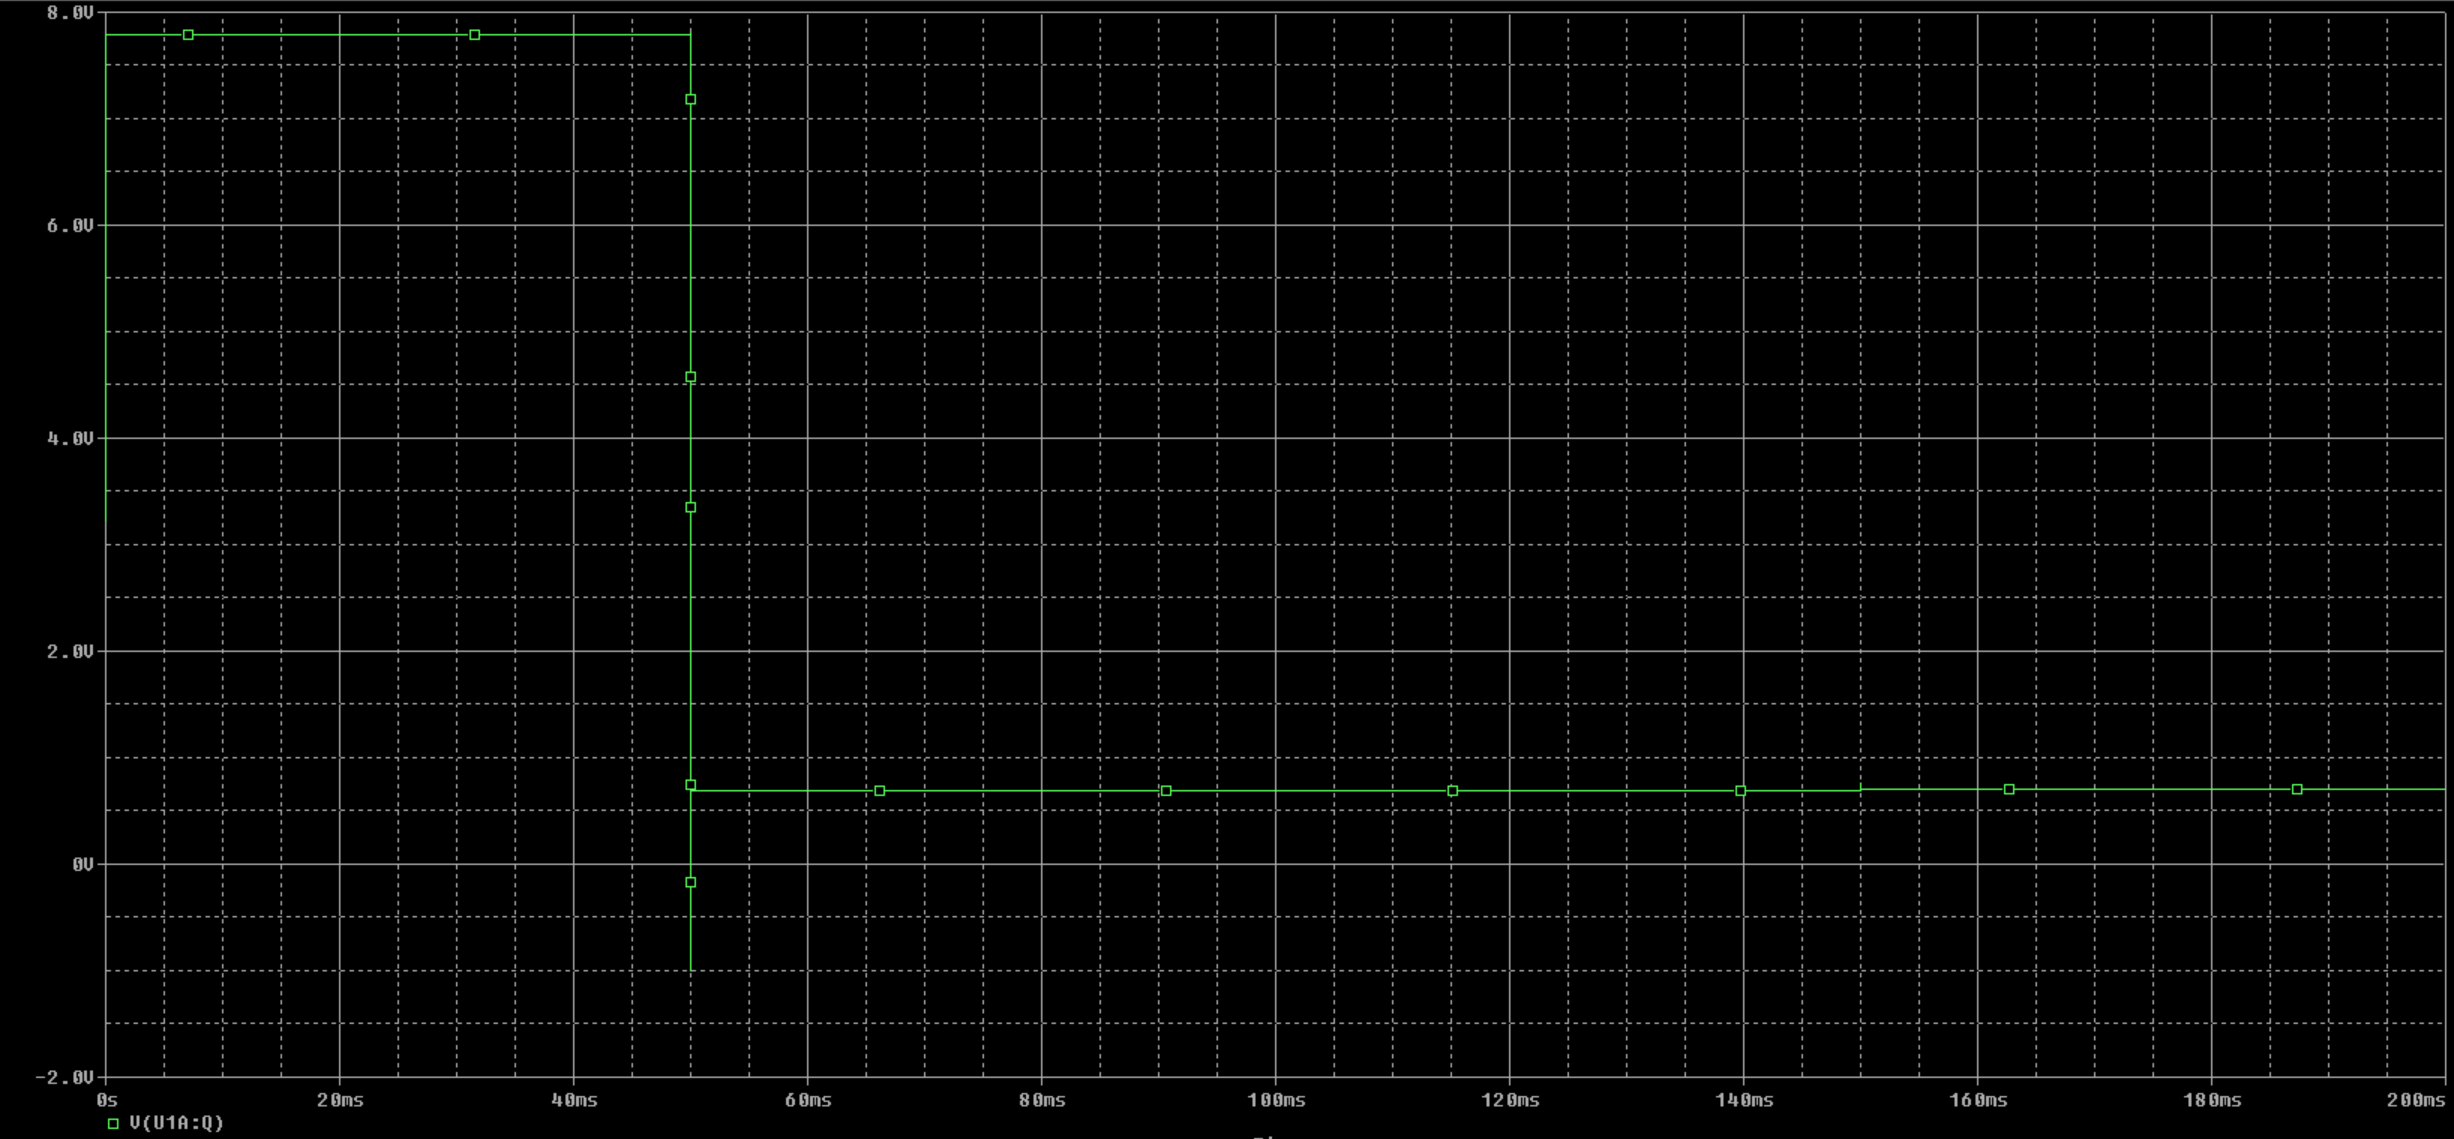
\includegraphics[width=\linewidth, height=0.30\textheight, keepaspectratio]{sim_arret}
			\caption{Simulation -- moteur \`a l'arr\^et}
		\end{subfigure}
		
		\caption{Logique de commande avec le CD4027N}
		\label{fig:commande}
	\end{figure}
	
	
	\section{Partie Puissance}
	
	\subsection{Alimentation du MCC}
	
	L'alimentation du moteur MCC est fournie par une source de tension continue
	externe, connect\'ee via le bornier \textbf{X3}. Le condensateur
	\textbf{C17} (330\,nF/100\,V) assure le filtrage des parasites haute
	fr\'equence. Cette tension est ensuite commut\'ee vers le moteur (bornier
	\textbf{X4}) par le MOSFET IRF530 selon le signal MLI.
	
	\subsection{Bloc de Puissance -- IRF530 et Diode de Roue Libre}
	
	Le MOSFET \textbf{IRF530} (Q6) re\c coit le signal MLI sur sa grille via
	les transistors de commande BC547/BC557. Lorsque $V_{GS} > V_{GS(th)}$,
	le canal s'ouvre et le courant traverse le moteur. La diode de roue libre
	\textbf{BYT08P} (D8), mont\'ee en antiparall\`ele avec le moteur, assure
	la continuit\'e du courant lors du blocage du MOSFET et le prot\`ege contre
	les surtensions inductives.
	
	\begin{figure}[H]
		\centering
		\begin{subfigure}[b]{\textwidth}
			\centering
			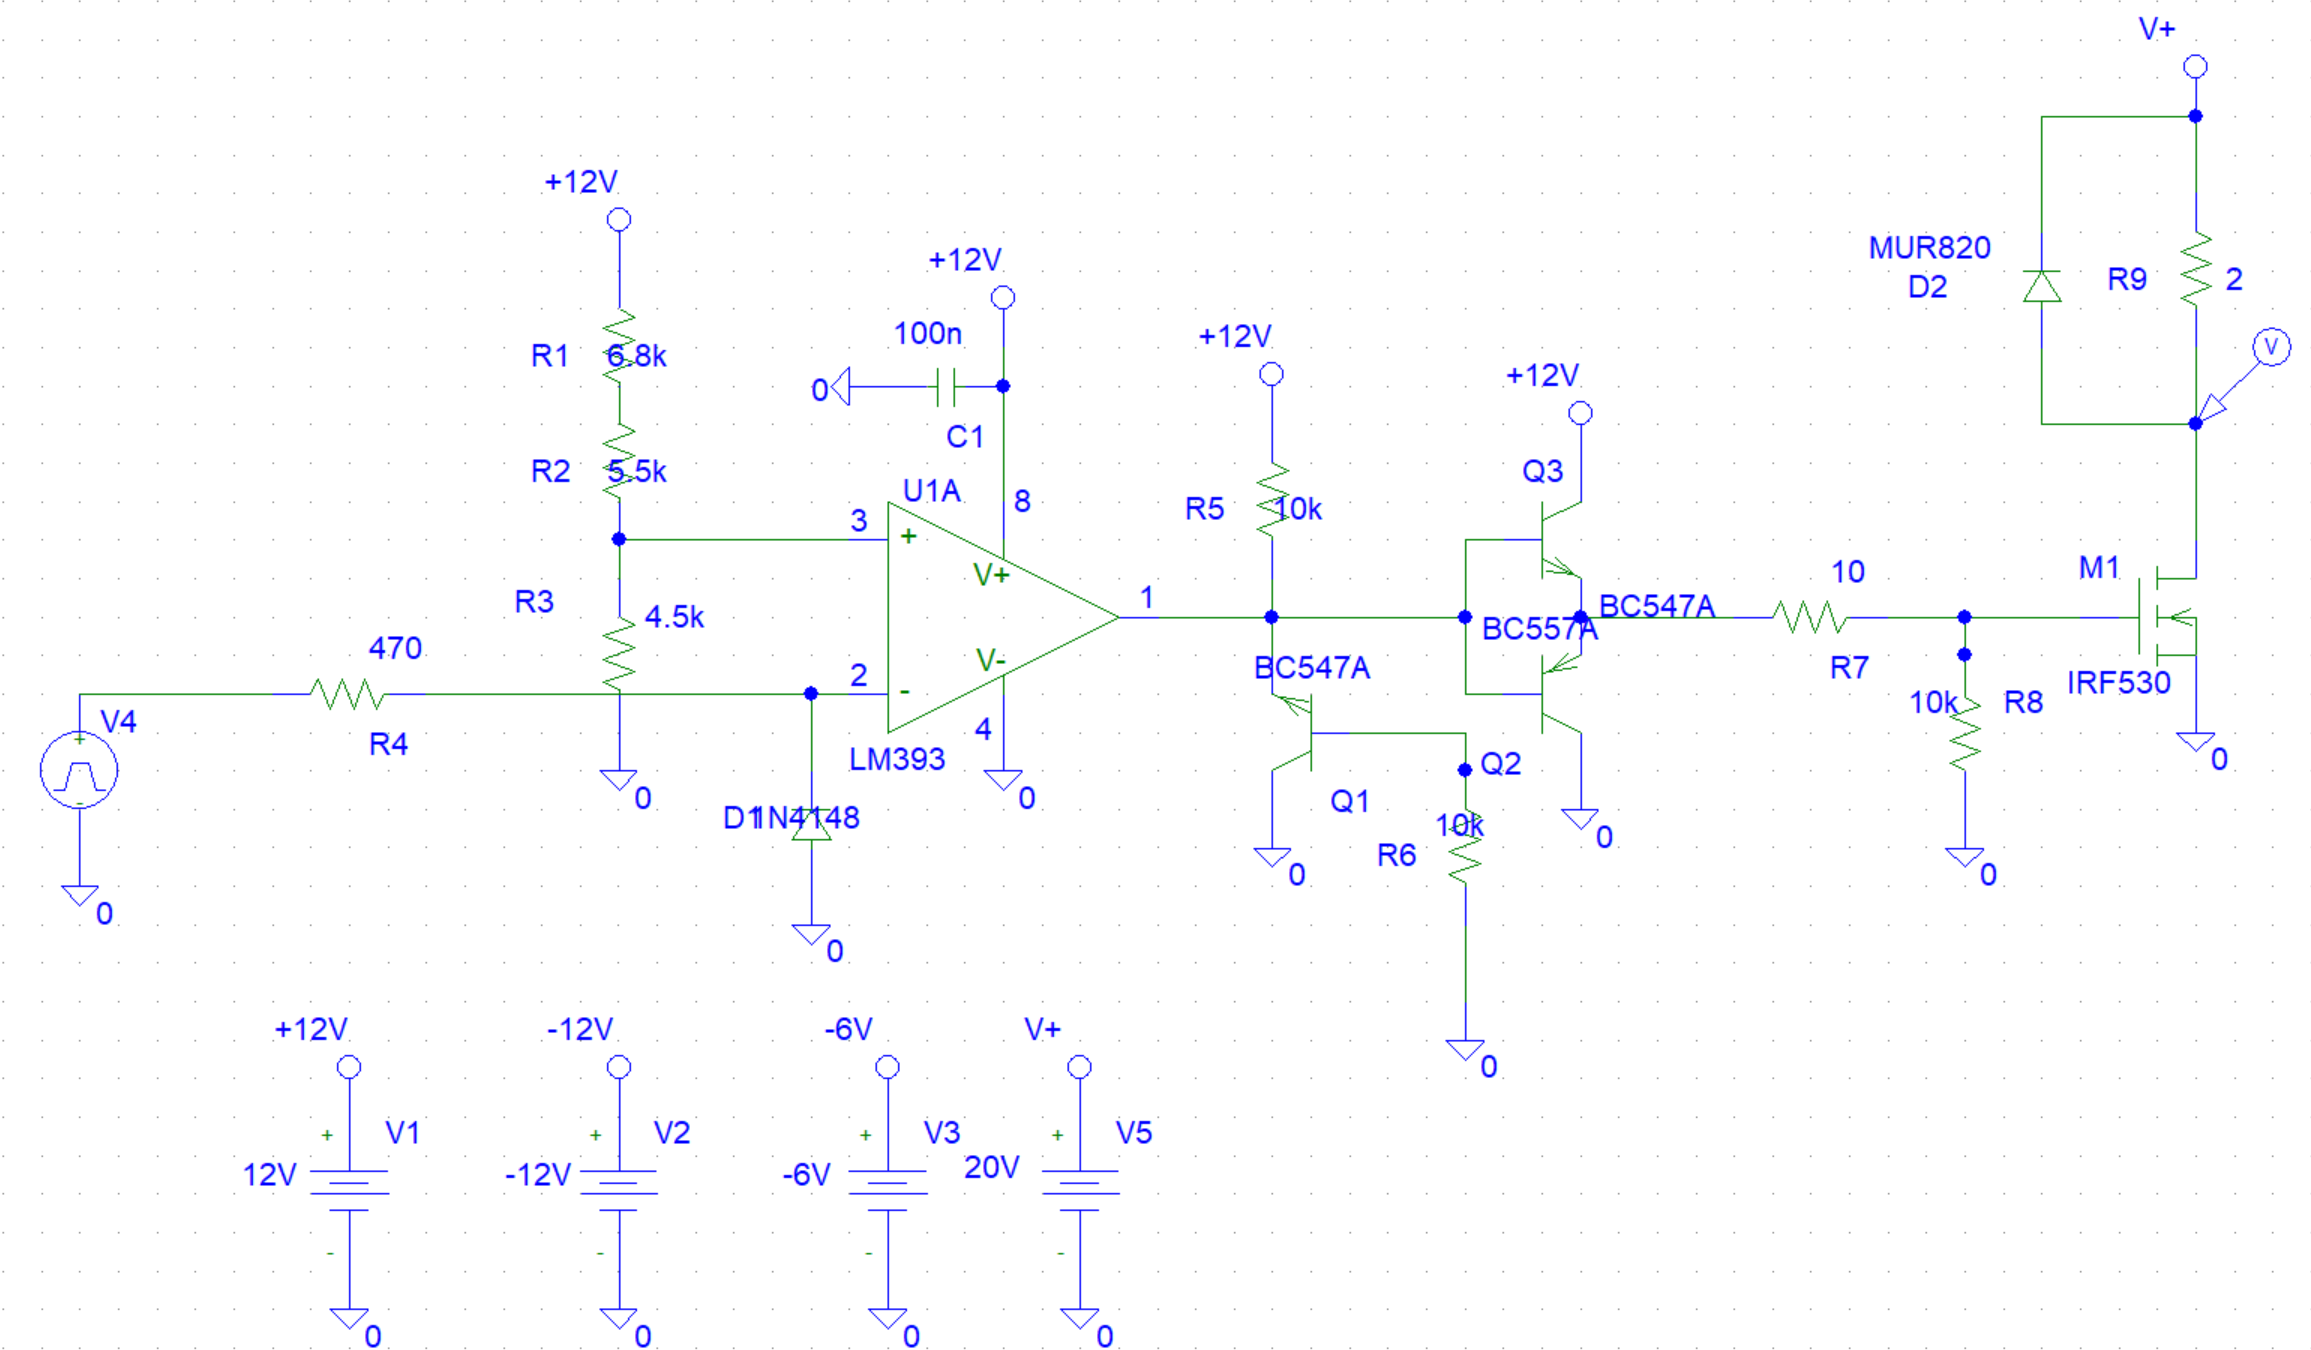
\includegraphics[width=\linewidth, height=0.35\textheight, keepaspectratio]{sch_MOT}
			\caption{Sch\'ema du bloc de puissance (PSpice)}
		\end{subfigure}
		
		\vspace{0.4cm}
		
		\begin{subfigure}[b]{\textwidth}
			\centering
			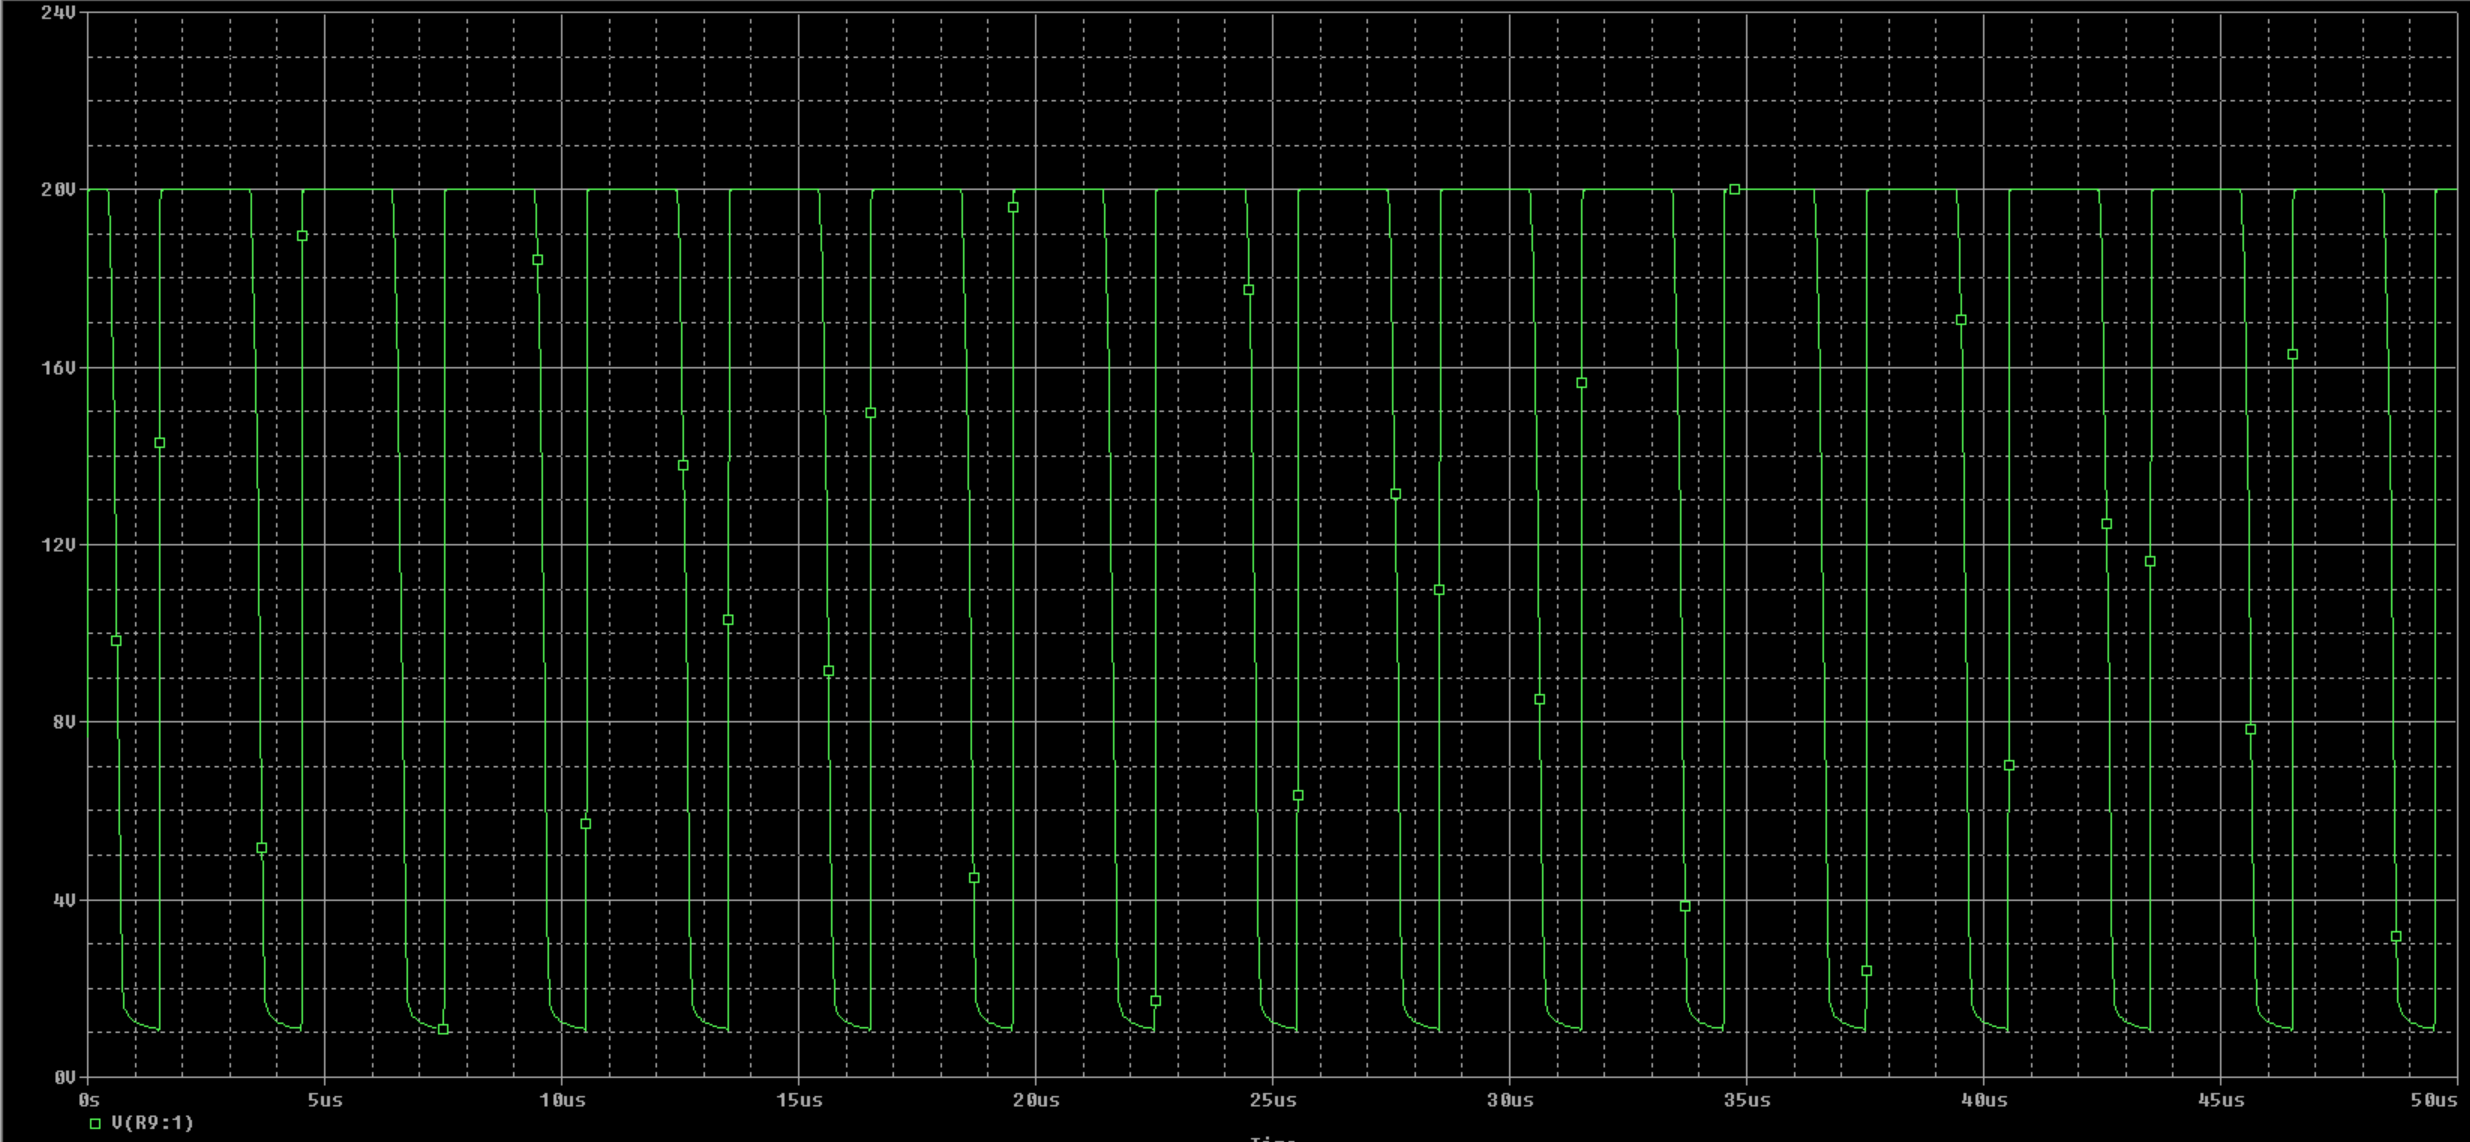
\includegraphics[width=\linewidth, height=0.35\textheight, keepaspectratio]{sim_mot}
			\caption{Signal MLI de puissance aux bornes du moteur}
		\end{subfigure}
		
		\caption{Simulation du bloc de puissance -- IRF530 sous PSpice}
		\label{fig:hacheur_serie}
	\end{figure}
	
	\subsection{Relais et Inversion du Sens de Rotation}
	
	Le relais \textbf{G2R-2} (K1), pilot\'e par Q7 (2N2222) depuis la bascule
	IC7B, permet d'inverser la polarit\'e aux bornes du moteur (bornier X4),
	r\'ealisant ainsi l'inversion du sens de rotation.
	
	\section{Conclusion}
	
	L'analyse th\'eorique des diff\'erents blocs fonctionnels montre la
	coh\'erence de la conception~: le NE555N g\'en\`ere le signal MLI, le
	$\mu$A741P conditionne la consigne, le LM393N assure la comparaison, le
	CD4027N g\`ere la logique de commande, et l'IRF530 commute la puissance
	vers le moteur via le bornier X3--X4.
	
	


	%%=========================================================


\chapter{R\'ealisation}

\begin{enumerate}
	\item \textbf{Simulation sur PSpice~:} chaque bloc simul\'e
	individuellement pour valider le comportement th\'eorique.
	
	\item \textbf{Sch\'ema sur EAGLE~:} saisie du sch\'ema complet avec
	les biblioth\`eques standard (rcl, linear, v-reg, diode, transistor).
	
	\begin{figure}[H]
		\centering
		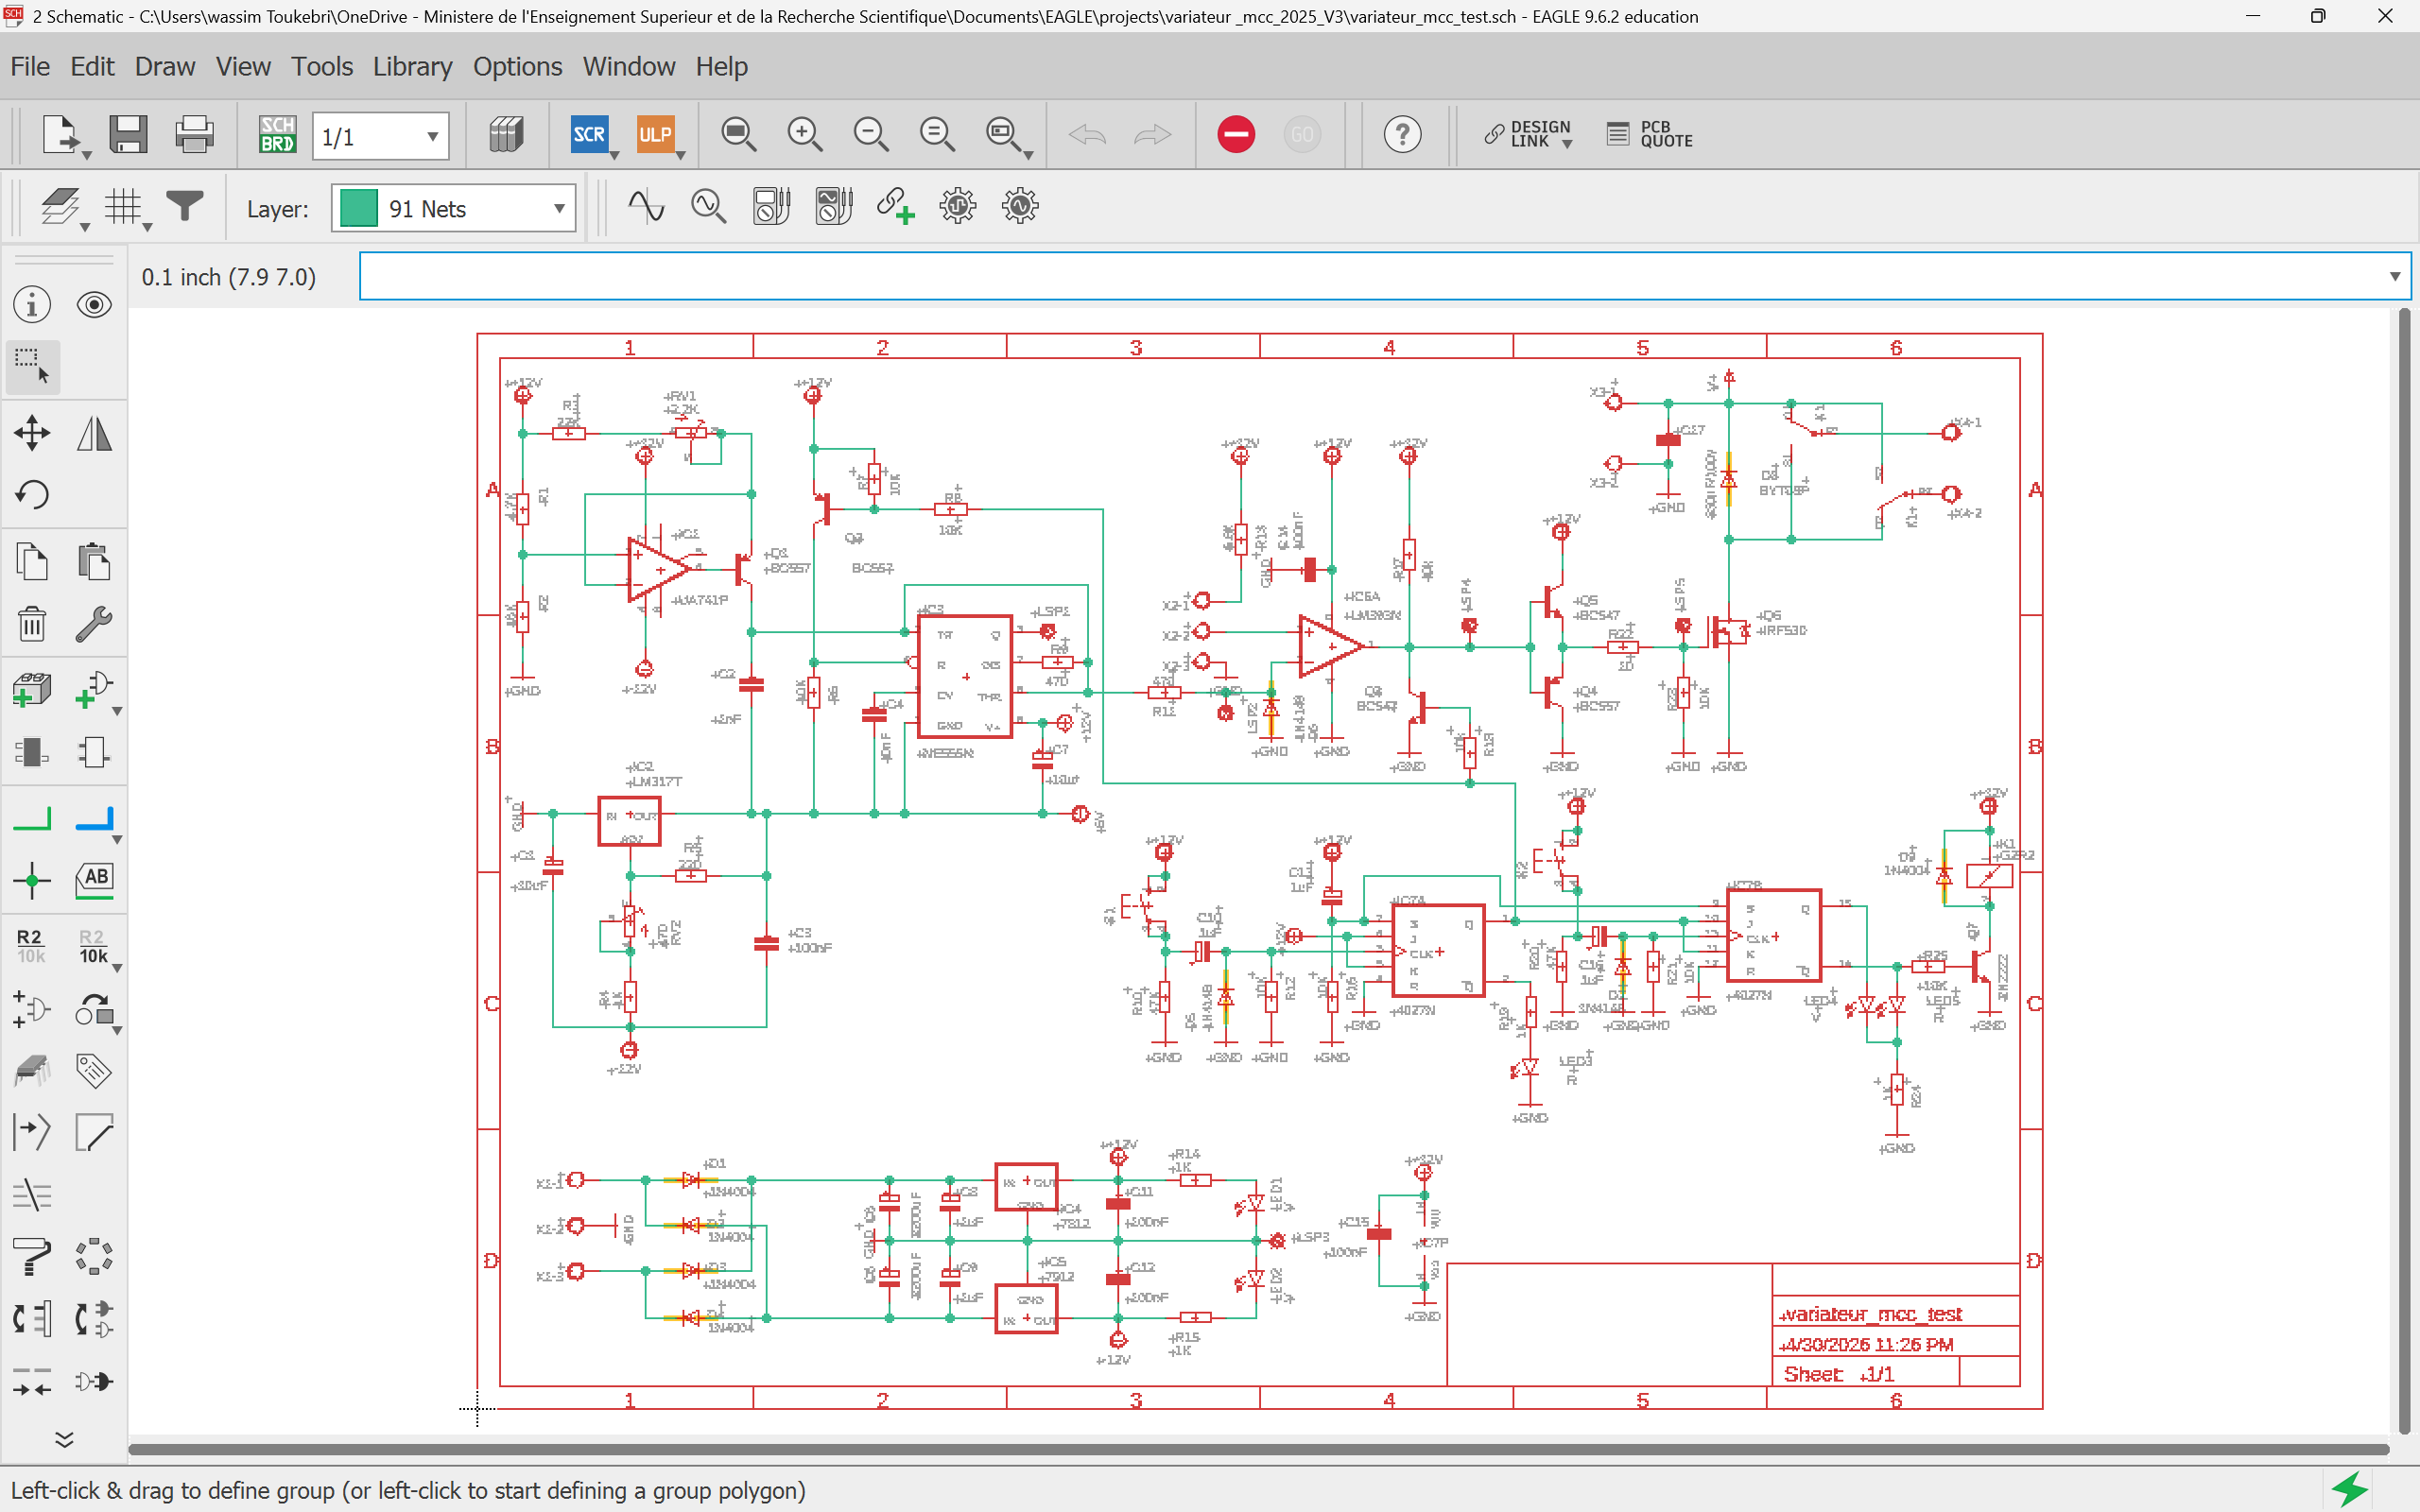
\includegraphics[width=\linewidth, height=0.35\textheight,
		keepaspectratio]{sch}
		\caption{Sch\'ema \'electrique r\'ealis\'e sous EAGLE}
		\label{fig:real_schema}
	\end{figure}
	
	
\item \textbf{Routage du PCB~:} apr\`es la saisie et la v\'erification
du sch\'ema, le routage du circuit imprim\'e a \'et\'e r\'ealis\'e sous
EAGLE. La carte est limit\'ee \`a un format de \textbf{120$\times$160\,mm}.

\textbf{Calcul de la largeur des pistes~:} pour d\'eterminer la largeur
n\'ecessaire des pistes selon le courant qu'elles doivent supporter, on
utilise la norme IPC recommand\'ee pour un PCB en cuivre 1\,oz avec une
\'el\'evation de temp\'erature de 10\,\textdegree C~:

\begin{table}[H]
	\centering
	\caption{Largeur des pistes selon le courant admissible (norme IPC,
		cuivre 1\,oz, $\Delta T = 10$\,\textdegree C)}
	\begin{tabular}{|c|c|c|l|}
		\hline
		\textbf{Courant (A)} & \textbf{Largeur (mil)} &
		\textbf{Largeur (mm)} & \textbf{Application dans notre carte} \\
		\hline
		1  & 10  & 0.25 & Signaux logiques (CD4027N, LM393N) \\
		2  & 30  & 0.76 & Pistes de signal g\'en\'eral \\
		3  & 50  & 1.27 & Alimentation commande ($\pm$12\,V) \\
		4  & 80  & 2.03 & Pistes puissance (IRF530, BYT08P) \\
		5  & 110 & 2.79 & Pistes puissance (pont redresseur) \\
		\hline
	\end{tabular}
	\label{tab:track_width}
\end{table}

\textbf{R\`egles de conception appliqu\'ees~:}
\begin{itemize}
	\item \textbf{Espacement~:} distance minimale entre pistes
	\'egale \`a la largeur d'une piste pour \'eviter les
	courts-circuits lors de la gravure.
	\item \textbf{Restring des pastilles~:} fix\'e \`a 40\,\% pour
	garantir une surface de soudure suffisante sans risque de
	court-circuit entre pastilles adjacentes.
	\item \textbf{Angles~:} tous les trac\'es sont orient\'es \`a
	45\textdegree~; les virages \`a 90\textdegree{} sont
	\'evit\'es pour r\'eduire les r\'eflexions du signal et
	faciliter la gravure chimique.
	\item \textbf{Straps (cavaliers)~:} le nombre de straps est
	limit\'e \`a 10. Les straps
	ne doivent pas croiser les pistes pour \'eviter les
	interf\'erences, et leur longueur ne d\'epasse pas 2\,cm
	(r\'ealis\'es avec les pattes coup\'ees des composants).
	\item \textbf{Marges~:} distance minimale maintenue entre les
	pistes, les bords de la carte et les trous de fixation.
	\item \textbf{Plan de masse~:} un plan de cuivre (copper pour)
	a \'et\'e ajout\'e sur la couche inf\'erieure pour r\'eduire
	le bruit \'electromagn\'etique et dissiper la chaleur.
	Les \textit{thermals} ont \'et\'e activ\'es pour faciliter
	la soudure. Les \textit{orphans} ont \'et\'e d\'esactiv\'es
	pour \'eviter les \^ilots de cuivre isol\'es.
	\item \textbf{S\'eparation commande/puissance~:} les zones
	analogiques ($\mu$A741P, LM393N) et num\'eriques (CD4027N)
	sont s\'epar\'ees physiquement des zones de puissance
	(IRF530, BYT08P) pour minimiser les couplages parasites.
	\item \textbf{Composants TO-220~:} l'IRF530, le LM317T et les
	r\'egulateurs 7812/7912 sont plac\'es en bordure de carte
	pour permettre la fixation de dissipateurs thermiques.
\end{itemize}

	\begin{figure}[H]
		\centering
		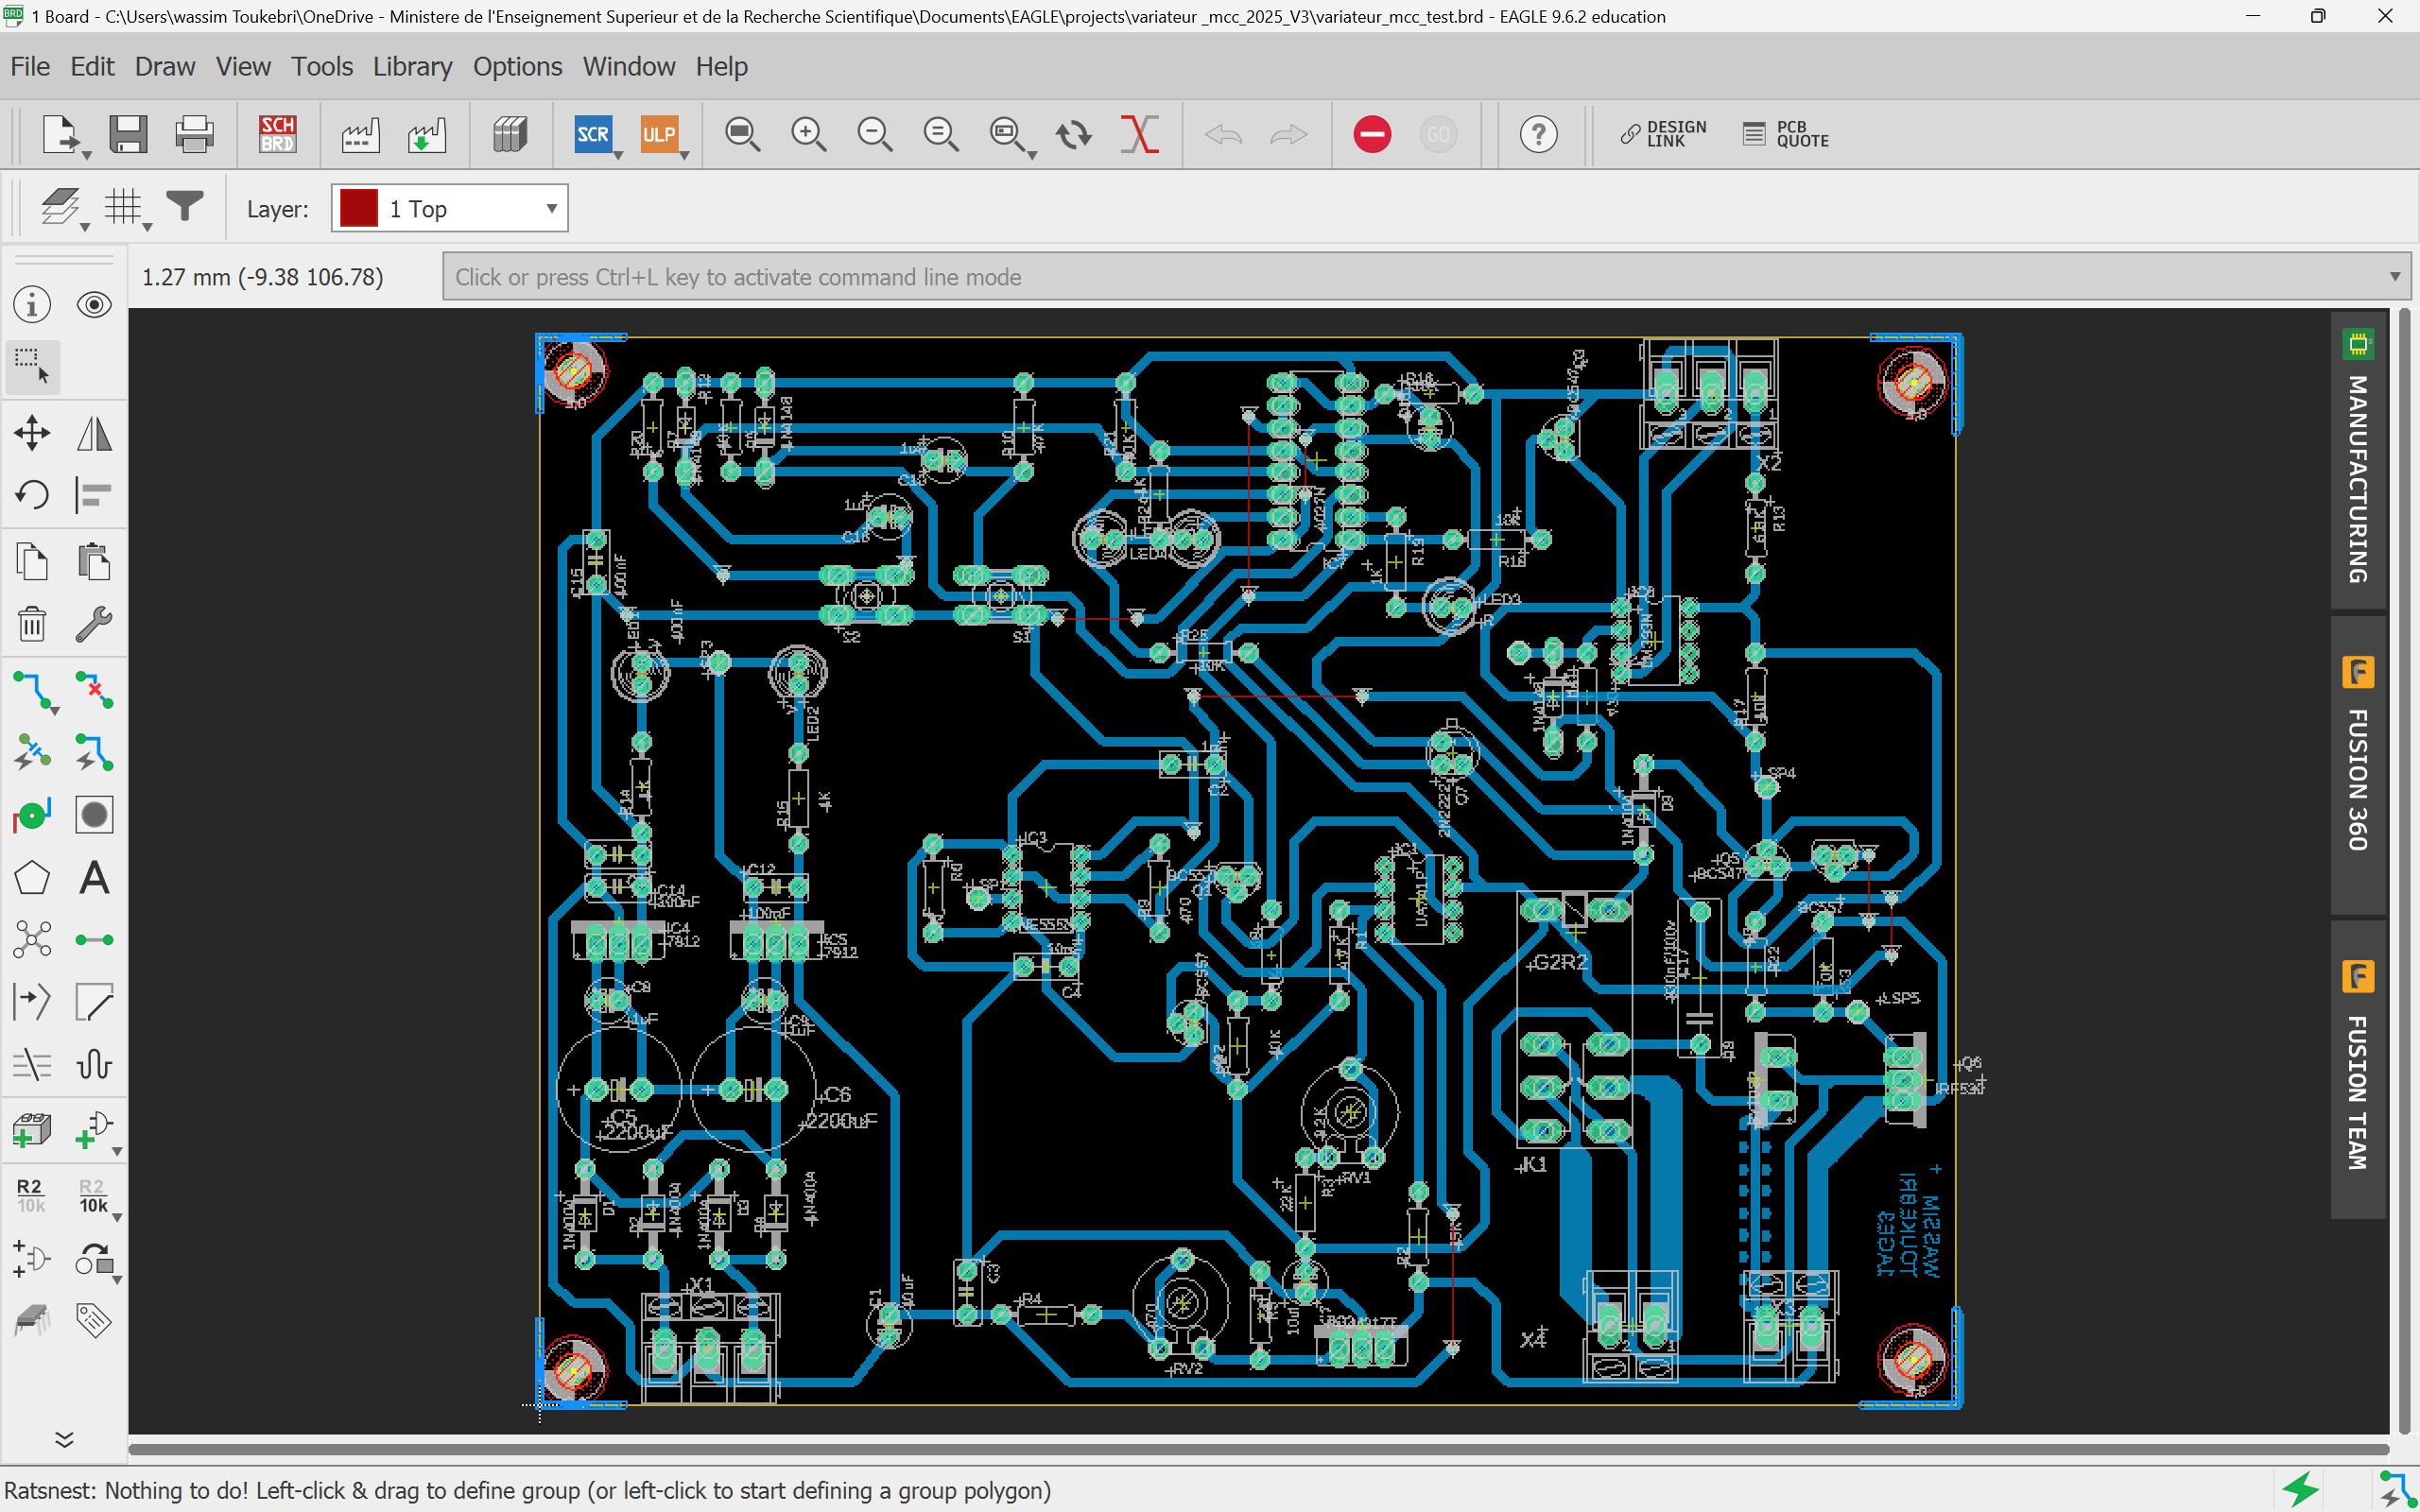
\includegraphics[width=\linewidth, height=0.35\textheight,
		keepaspectratio]{board}
		\caption{Routage du circuit imprim\'e r\'ealis\'e sous EAGLE --
			vue composants et pistes}
		\label{fig:real_routage}
	\end{figure}
	
	
	\item \textbf{Vérification DRC (Design Rule Check)~:} après le routage, une vérification DRC est effectuée sous EAGLE pour s'assurer du respect des règles de fabrication. Les paramètres configurés sont résumés dans le tableau suivant~:
	
	\begin{table}[H]
		\centering
		\caption{Paramètres DRC configurés sous EAGLE}
		\label{tab:drc}
		\renewcommand{\arraystretch}{1.3}
		\begin{tabular}{|l|l|c|}
			\hline
			\textbf{Catégorie} & \textbf{Paramètre} & \textbf{Valeur} \\
			\hline
			\multirow{4}{*}{Clearance (signaux différents)} 
			& Wire -- Wire   & 40\,mil \\
			& Wire -- Pad    & 40\,mil \\
			& Pad -- Via     & 40\,mil \\
			& Via -- Via     & 40\,mil \\
			\hline
			Clearance (même signal) 
			& Smd -- Smd/Pad/Via & 6\,mil \\
			\hline
			\multirow{2}{*}{Distance}
			& Cuivre / Dimension & 40\,mil \\
			& Perçage / Trou     & 6\,mil \\
			\hline
			\multirow{2}{*}{Tailles minimales}
			& Largeur de piste   & 40\,mil \\
			& Diamètre de perçage & 0{,}7\,mm \\
			\hline
			\multirow{2}{*}{Annular Ring -- Pastilles}
			& Top / Inner (min, \%) & 10\,mil, 25\,\% \\
			& Bottom (min, \%)      & 10\,mil, 50\,\% \\
			\hline
			\multirow{2}{*}{Annular Ring -- Vias}
			& Outer / Inner (min, \%) & 8\,mil, 25\,\% \\
			& Micro Via (min, \%)     & 4\,mil, 25\,\% \\
			\hline
			\multirow{2}{*}{Masks}
			& Stop mask (min, \%) & 4\,mil, 100\,\% \\
			& Cream mask          & 0\,mil \\
			\hline
		\end{tabular}
	\end{table}
	
	
	
\subsection{Fabrication du PCB -- Processus d'Insolation}

La fabrication de la carte utilise le proc\'ed\'e d'\textbf{insolation
	aux UV}. Ce processus se d\'eroule en trois \'etapes successives~:

\begin{enumerate}
	\item \textbf{Insolation aux UV~:} le typon (film transparent
	imprim\'e avec le motif des pistes) est pos\'e sur la plaque
	\'epoxy pr\'esensibilis\'ee, puis expos\'e aux ultraviolets dans
	une \textbf{insoleuse}. Les zones expos\'ees aux UV voient leur
	r\'esine photosensible se polym\'eriser.
	
	\begin{figure}[H]
		\centering
		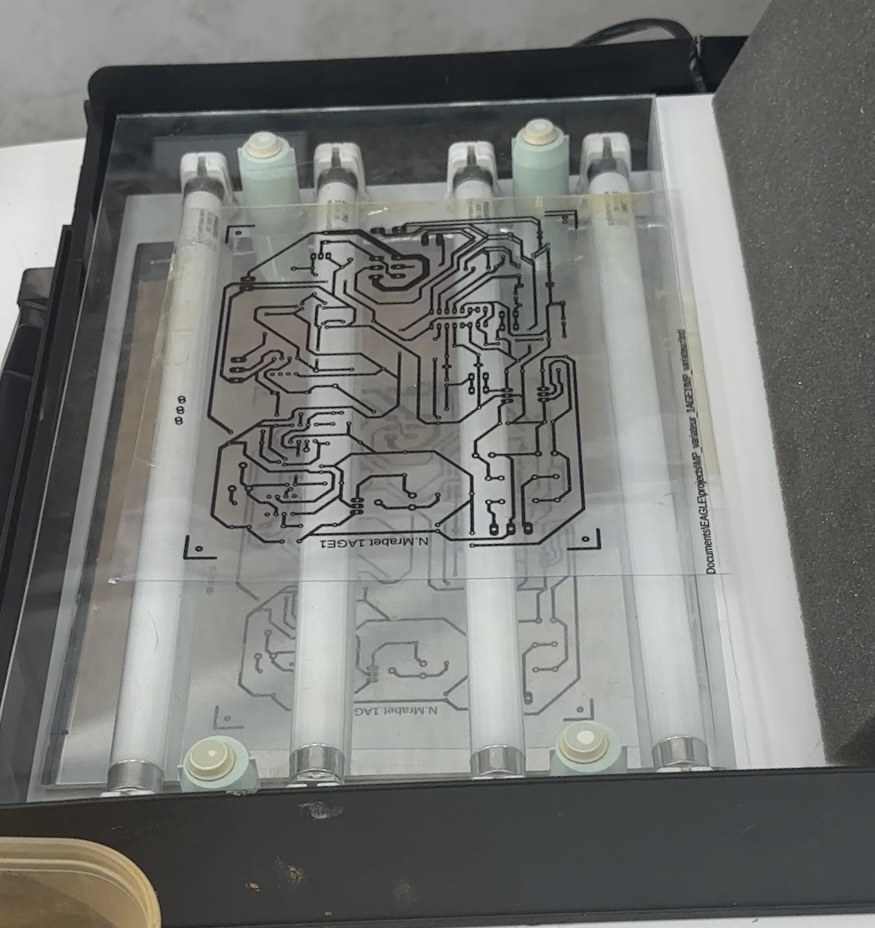
\includegraphics[width=\linewidth, height=0.25\textheight,
		keepaspectratio]{UV}
		\caption{Insolation aux UV de la plaque pr\'esensibilis\'ee}
		\label{fig:insoleuse}
	\end{figure}
	
	\item \textbf{D\'eveloppement \`a l'hydroxyde de sodium~:} apr\`es
	l'insolation, la carte est plong\'ee dans un bain d'\textbf{hydroxyde
		de sodium} (NaOH). Ce r\'ev\'elateur dissout la r\'esine non
	polym\'eris\'ee (zones non expos\'ees aux UV), mettant \`a nu le
	cuivre dans ces zones.
	
	\begin{figure}[H]
		\centering
		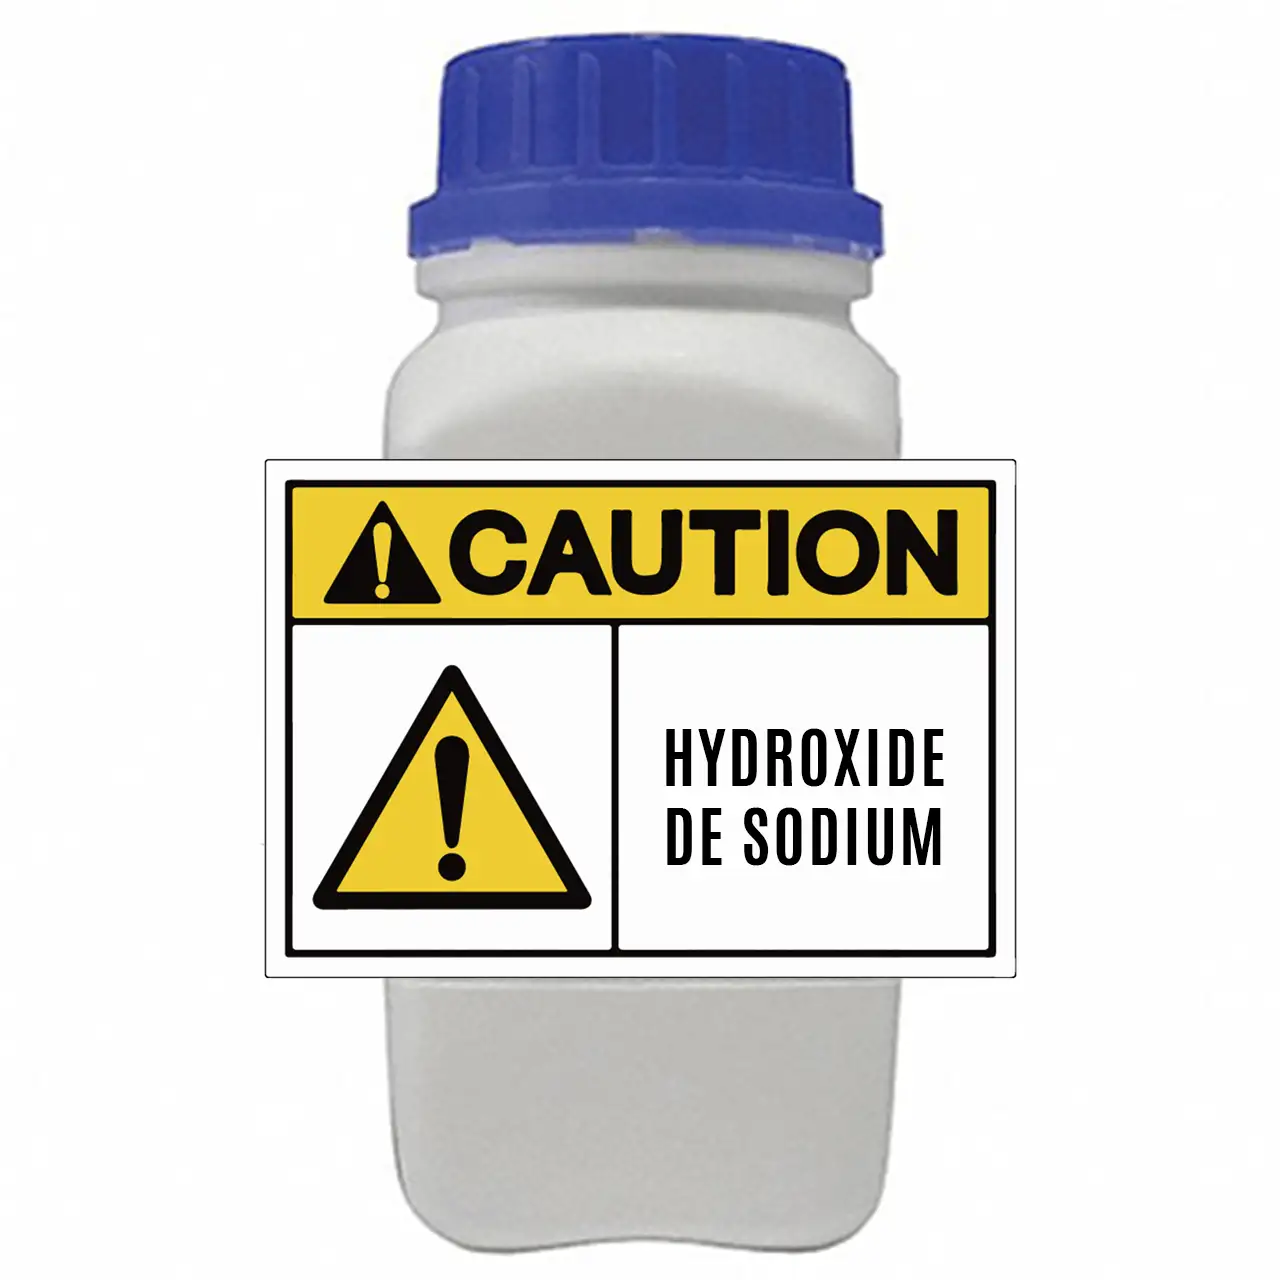
\includegraphics[width=\linewidth, height=0.25\textheight,
		keepaspectratio]{hydro}
		\caption{D\'eveloppement au bain d'hydroxyde de sodium (NaOH)}
		\label{fig:hydro}
	\end{figure}
	
	\item \textbf{Gravure au perchlorure de fer~:} la carte est
	ensuite plong\'ee dans un bain de \textbf{perchlorure de fer}
	(FeCl\textsubscript{3}). Ce r\'eactif attaque et dissout le cuivre
	non prot\'eg\'e par la r\'esine, laissant uniquement les pistes
	du circuit imprim\'e. La pr\'esence d'un plan de masse dans notre
	conception r\'eduit la quantit\'e de cuivre \`a graver, diminuant
	ainsi le temps d'exposition n\'ecessaire.
	
	\begin{figure}[H]
		\centering
		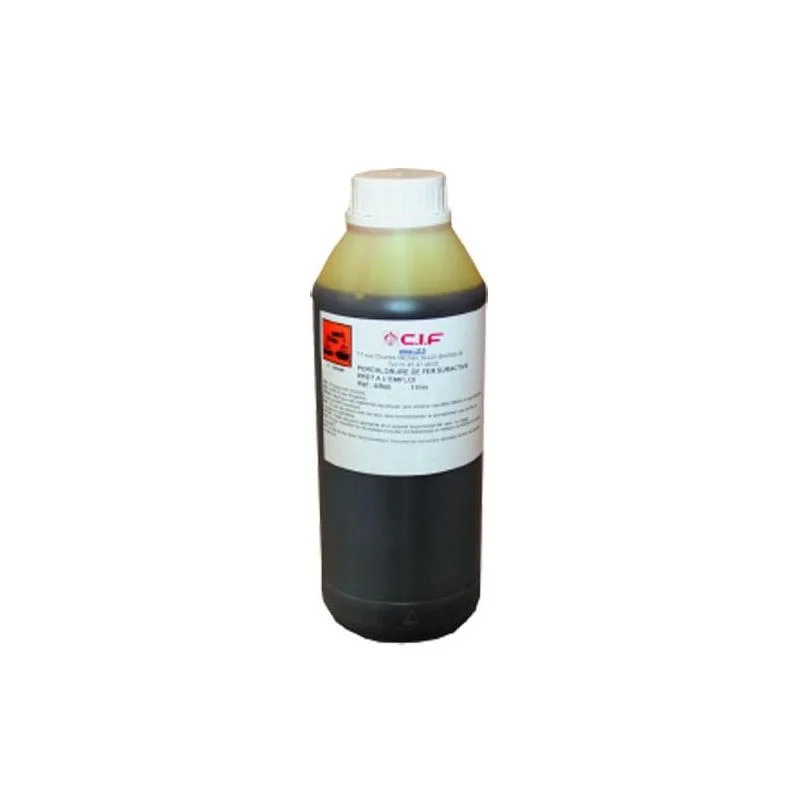
\includegraphics[width=\linewidth, height=0.25\textheight,
		keepaspectratio]{perch}
		\caption{Gravure au bain de perchlorure de fer
			(FeCl\textsubscript{3})}
		\label{fig:perch}
	\end{figure}
	
\end{enumerate}

Une fois la gravure termin\'ee, la carte est rinc\'ee \`a l'eau, puis
les trous de passage des composants sont per\c c\'es avant de passer
\`a l'\'etape de soudure.
	
	\item \textbf{Soudure~:} insertion et soudure des composants
	traversants avec pr\'ecision.
	
	\begin{figure}[H]
		\centering
		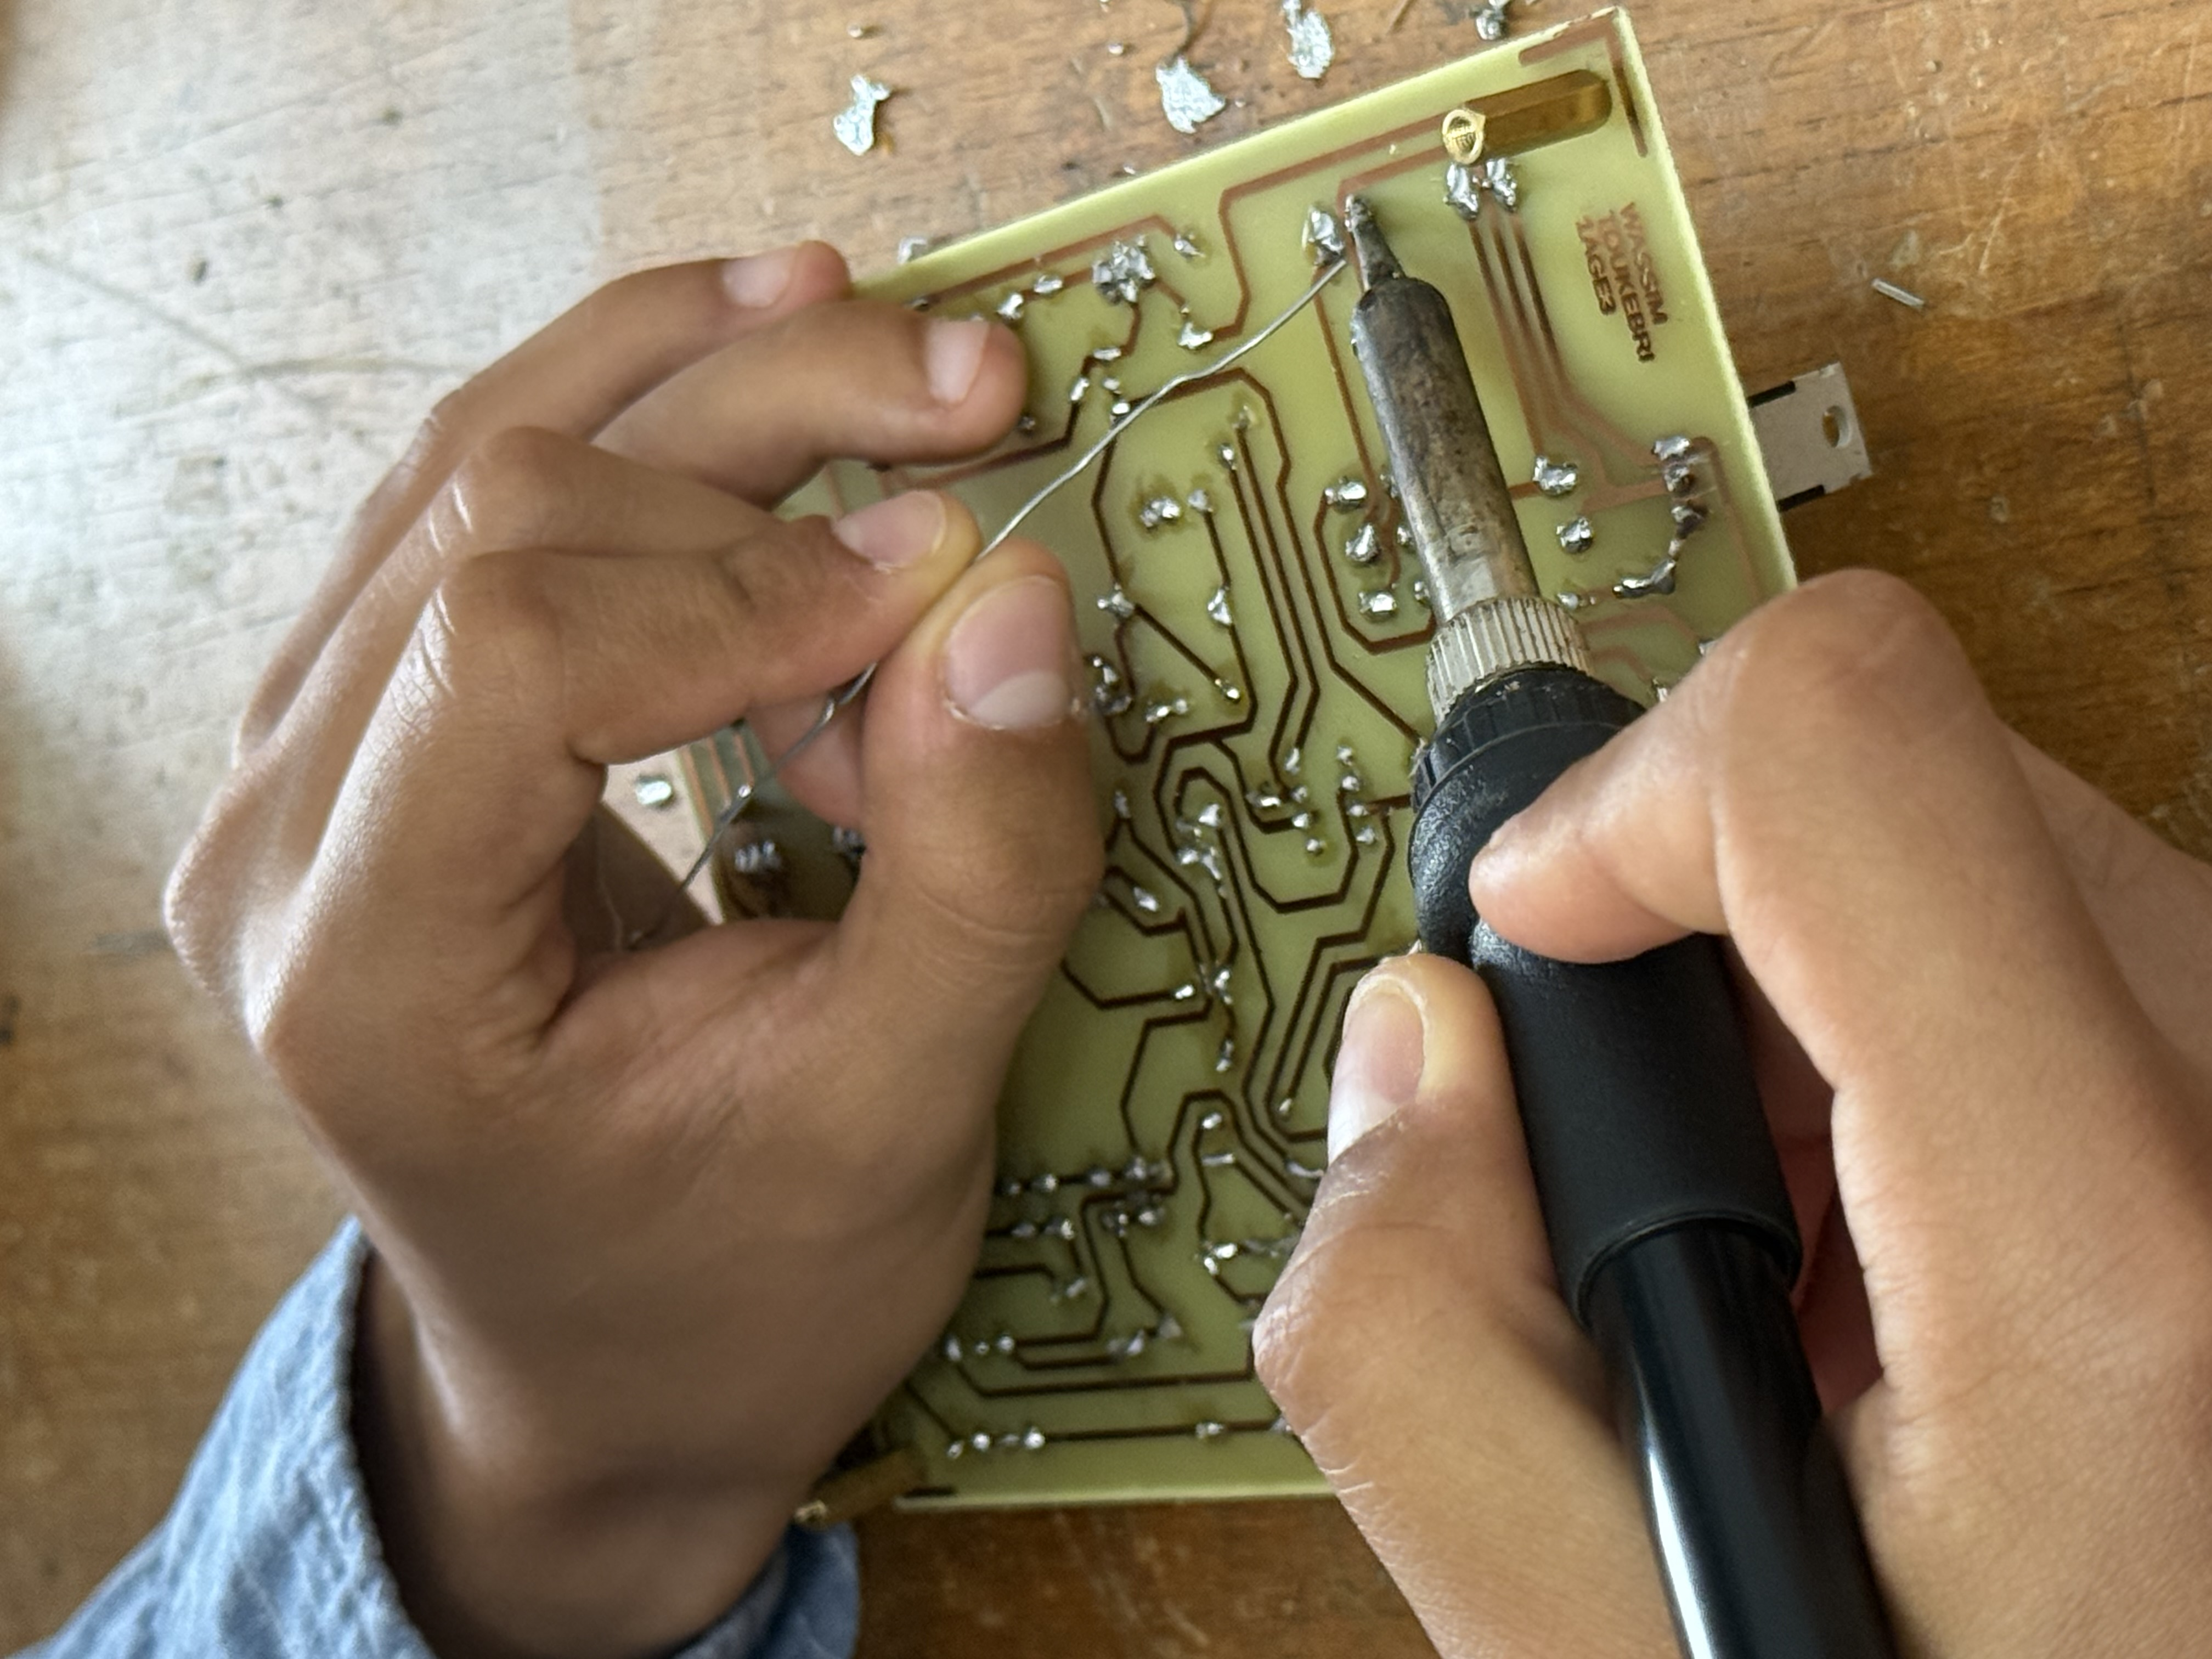
\includegraphics[width=\linewidth, height=0.4\textheight,
		keepaspectratio]{soudage}
				\vspace{0.5cm}
		\caption{Soudage des composants sur la carte}
		\label{fig:soudage}
	\end{figure}
	
	\item \textbf{Test de continuit\'e~:} v\'erification au multim\`etre
	de toutes les connexions de la carte pour d\'etecter les courts-circuits
	ou les soudures d\'efectueuses avant la mise sous tension.
	
	
	\item \textbf{Tests fonctionnels~:} test de l'alimentation puis
	branchement du moteur, visualisation du signal MLI \`a l'oscilloscope
	sur les points de test LSP.
	
	\begin{figure}[H]
		\centering
		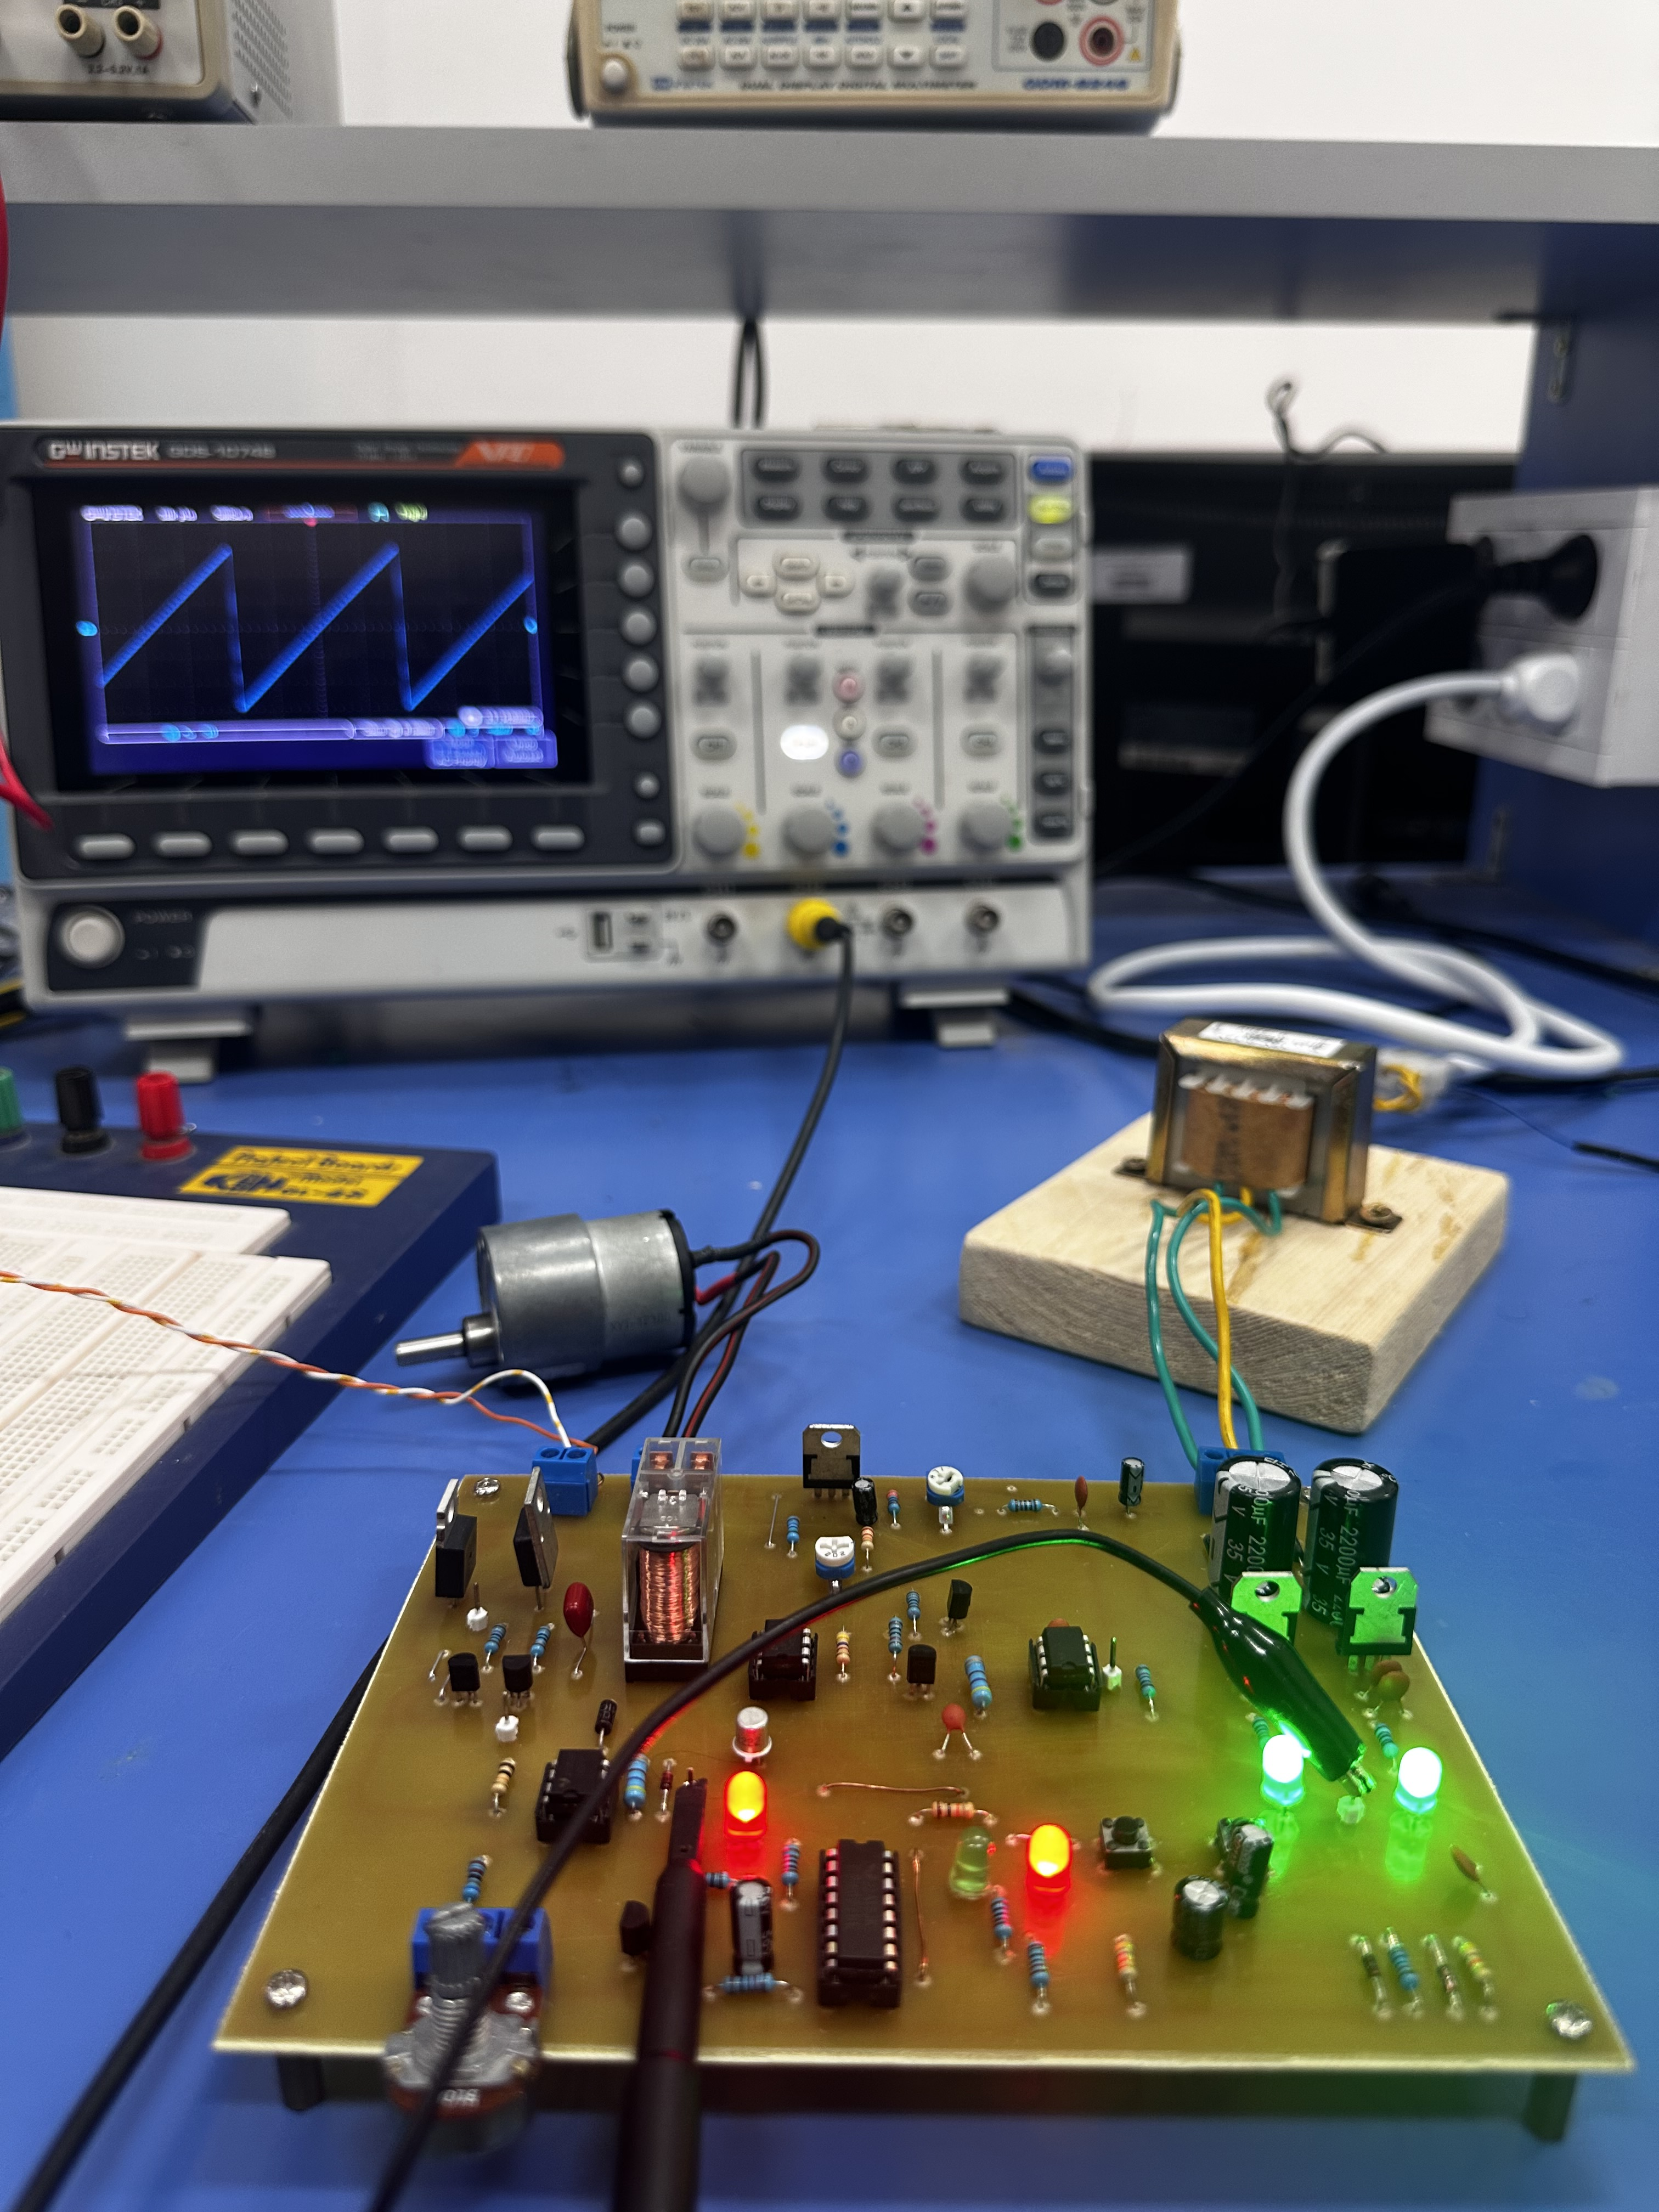
\includegraphics[width=\linewidth, height=0.5\textheight,
		keepaspectratio]{fin}
			\vspace{0.5cm}
		\caption{Carte finale assembl\'ee et test\'ee}
		\label{fig:carte_finale}
	\end{figure}
	
\end{enumerate}


	%%----------------------------------------------------------
	
\section{Mesures à l'Oscilloscope -- Points de Test LSP}


\begin{figure}[H]
	\centering
	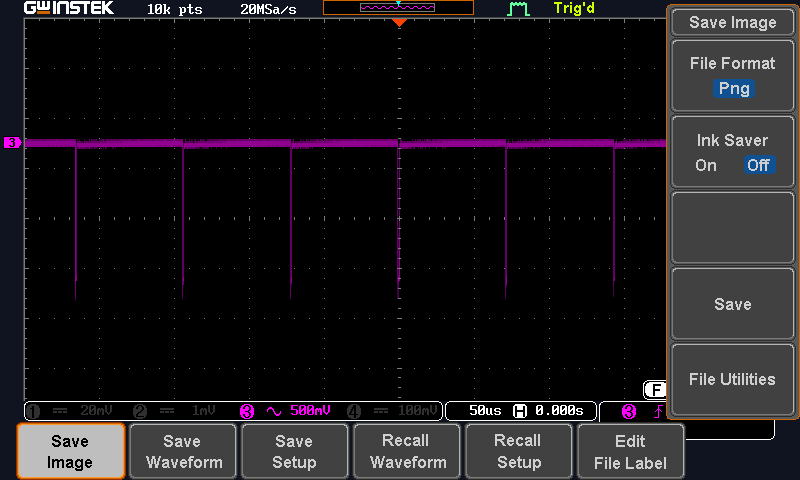
\includegraphics[width=\linewidth, height=0.25\textheight, keepaspectratio]{LSP1}
	\caption{LSP1}
	\label{fig:lsp1}
\end{figure}


\begin{figure}[H]
	\centering
	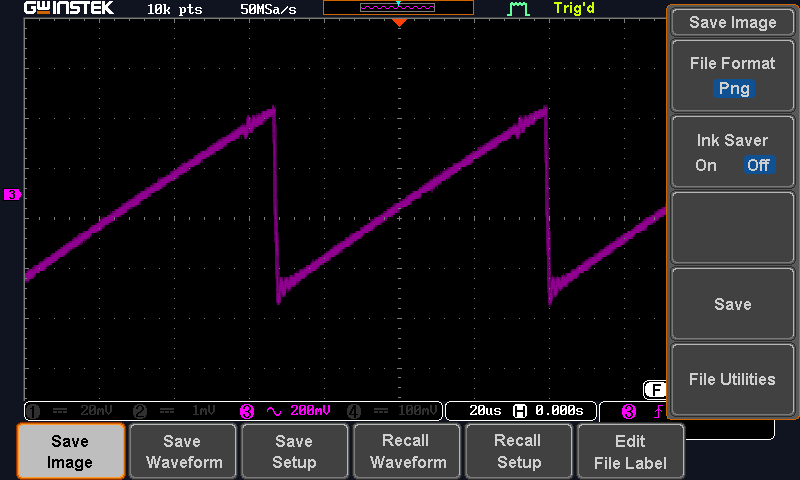
\includegraphics[width=\linewidth, height=0.25\textheight, keepaspectratio]{LSP2}
	\caption{LSP2}
	\label{fig:lsp2}
\end{figure}


\begin{figure}[H]
	\centering
	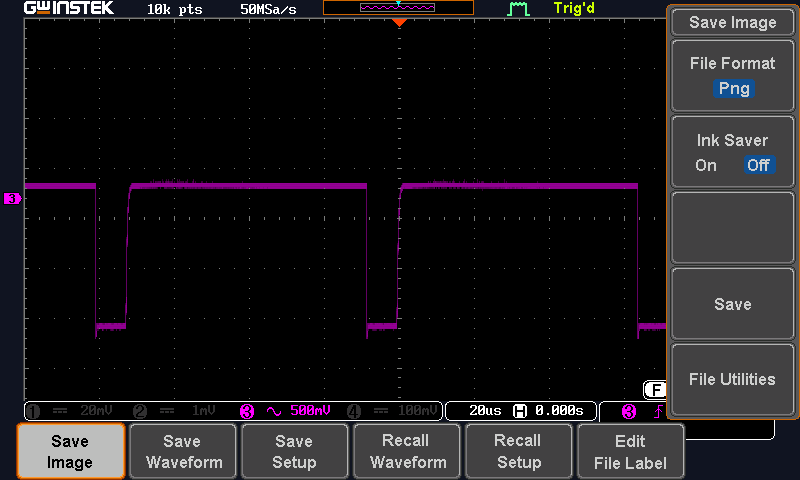
\includegraphics[width=\linewidth, height=0.25\textheight, keepaspectratio]{LSP4}
	\caption{LSP4}
	\label{fig:lsp4}
\end{figure}

\begin{figure}[H]
	\centering
	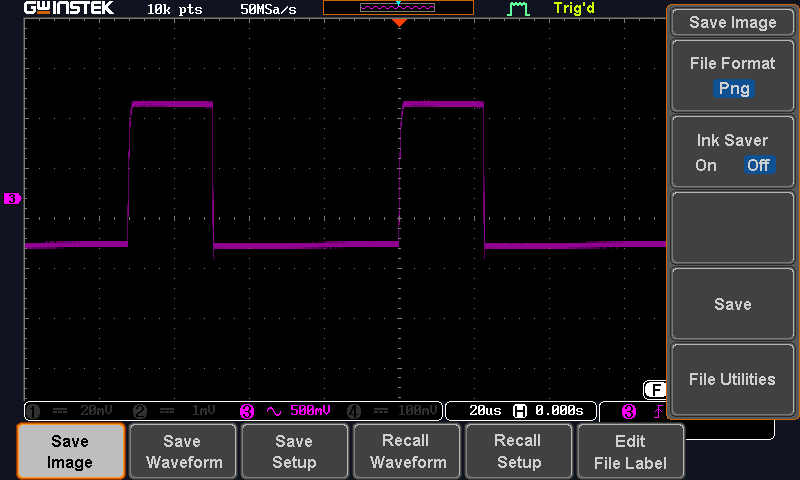
\includegraphics[width=\linewidth, height=0.25\textheight, keepaspectratio]{LSP5}
	\caption{LSP5}
	\label{fig:lsp5}
\end{figure}
	
	%%=========================================================
	\appendix
	\chapter{Dossier Technique}
	
	\newpage
	\section*{Sch\'ema \'Electrique Complet}
	\addcontentsline{toc}{section}{Sch\'ema \'Electrique}
	
	\begin{landscape}
		\thispagestyle{fancy}
		\begin{figure}[H]
			\centering
			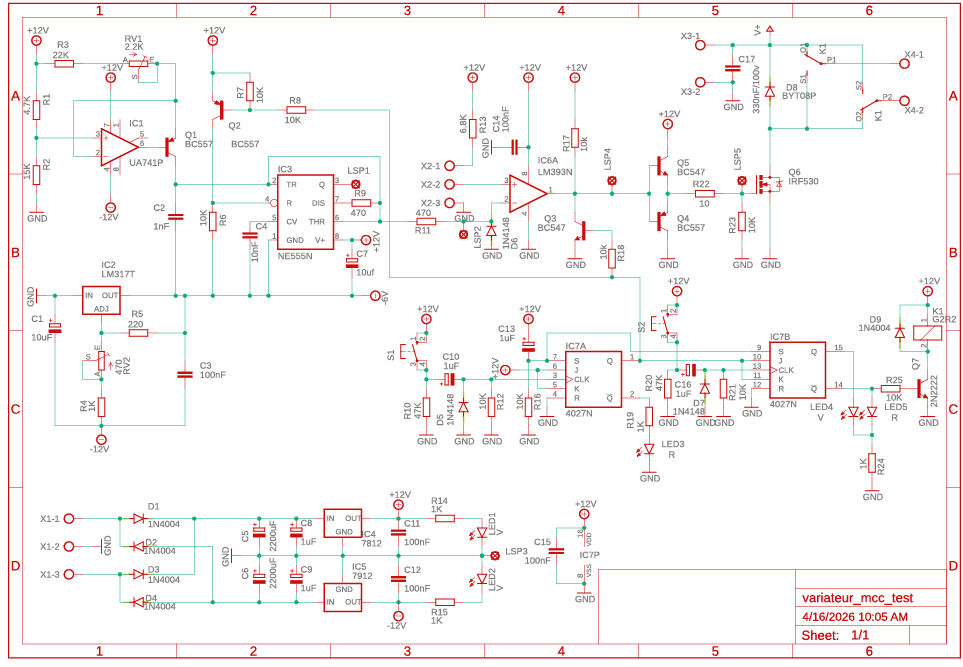
\includegraphics[width=\linewidth, height=0.92\textheight, keepaspectratio]{schema_eagle}
			\caption{Sch\'ema \'electrique complet du variateur MCC -- EAGLE}
			\label{fig:schema_eagle}
		\end{figure}
	\end{landscape}
	
	\newpage
	\section*{Sch\'ema d'implentation}
	\addcontentsline{toc}{section}{Sch\'ema d'implentation}
	\begin{figure}[H]
		\centering
		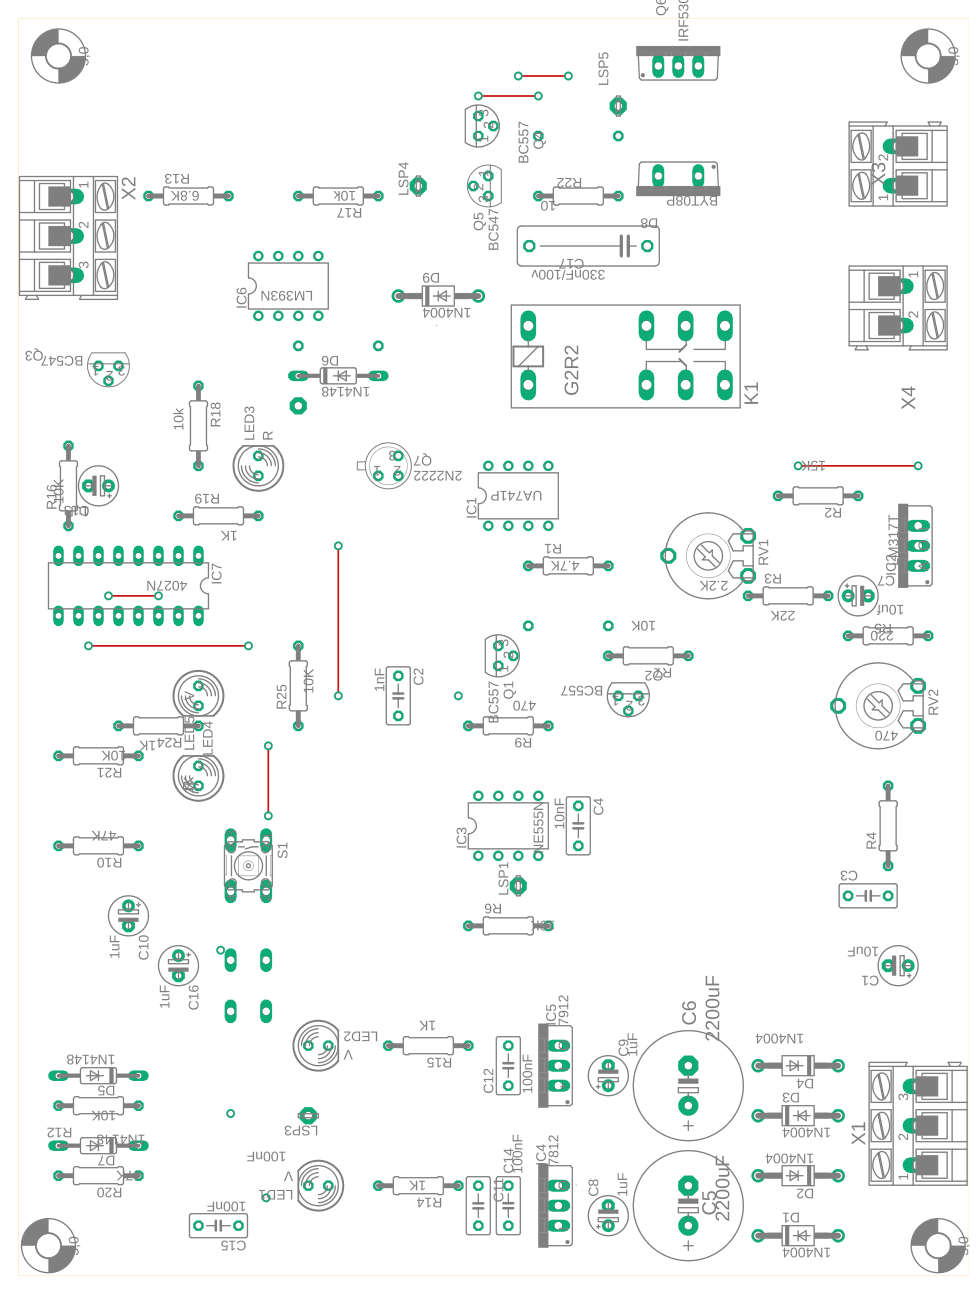
\includegraphics[width=\linewidth, height=0.92\textheight, keepaspectratio]{sch_imp}
		\caption{Fichier board EAGLE -- vue sur l'emplacement des composants }
		\label{fig:Sch\'ema d'implentation}
	\end{figure}
	
	\newpage
	\section*{Routage (Typon)}
	\addcontentsline{toc}{section}{Routage}
	\begin{figure}[H]
		\centering
		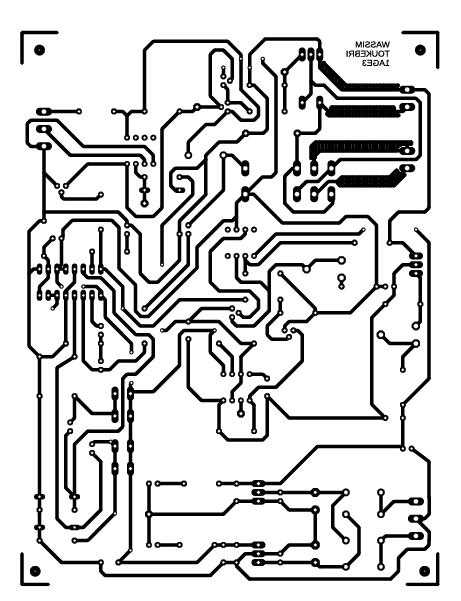
\includegraphics[width=\linewidth, height=0.92\textheight, keepaspectratio]{pcb_routage}
		\caption{Typon du circuit imprim\'e -- couche cuivre}
		\label{fig:pcb_routage}
	\end{figure}
	
	\section*{Board (PCB)}
	\addcontentsline{toc}{section}{Board}
	\begin{figure}[H]
		\centering
		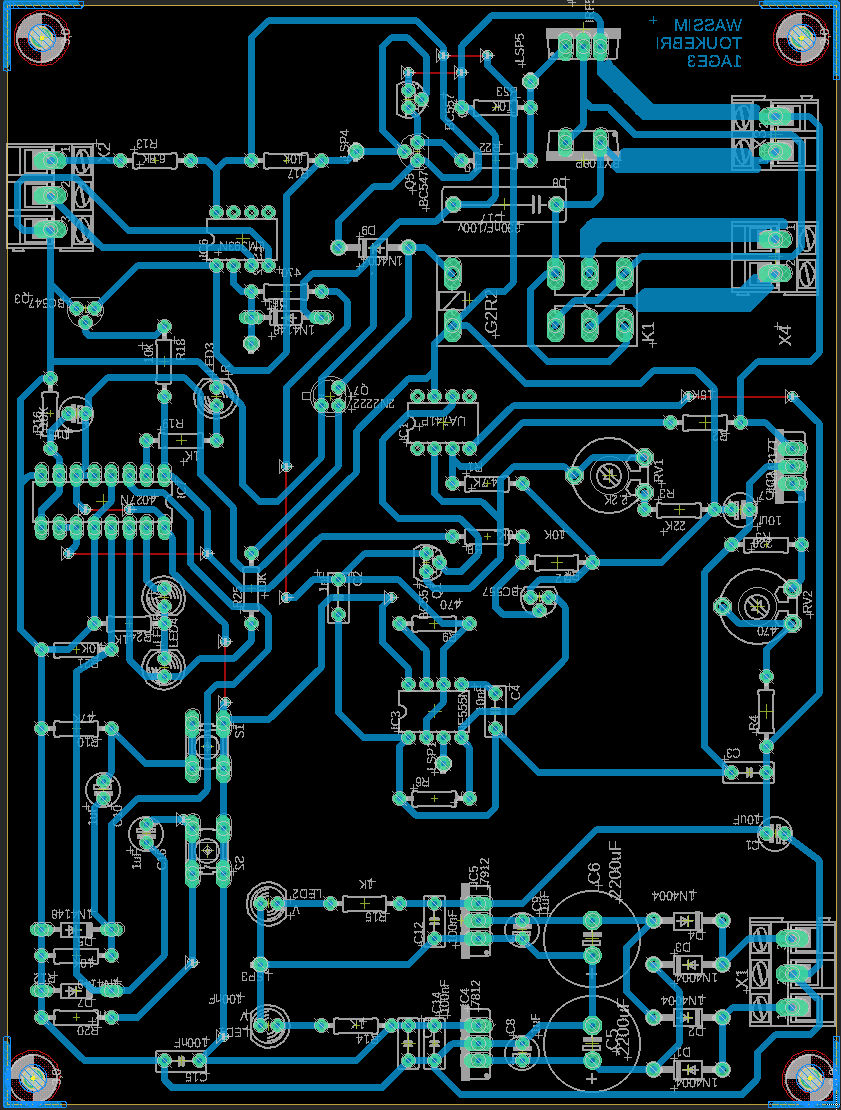
\includegraphics[width=\linewidth, height=0.92\textheight, keepaspectratio]{pcb_board}
		\caption{Fichier board EAGLE -- vue composants et pistes}
		\label{fig:pcb_board}
	\end{figure}
	
	
	\newpage
	\section*{Liste des Composants (BOM)}
	\addcontentsline{toc}{section}{Liste des Composants}
	
	% Colonnes : Réf (3cm) | Valeur (3cm) | Boîtier (3.5cm) | Description (reste)
	\begin{longtable}{|p{3.8cm}|p{3cm}|p{3.5cm}|p{5.5cm}|}
		\caption{Liste compl\`ete des composants -- variateur\_mcc\_2025\_V3} \label{tab:bom} \\
		\hline
		\textbf{R\'ef\'erence} & \textbf{Valeur} & \textbf{Bo\^itier} & \textbf{Description} \\
		\hline
		\endfirsthead
		\hline
		\textbf{R\'ef\'erence} & \textbf{Valeur} & \textbf{Bo\^itier} & \textbf{Description} \\
		\hline \endhead
		\hline \multicolumn{4}{r}{\textit{Suite page suivante\ldots}} \\ \endfoot
		\hline \endlastfoot
		%--- Condensateurs ---
		C1, C7                        & 10\,$\mu$F      & E2,5-5        & Condensateur polaris\'e \\
		C2                            & 1\,nF           & C050-030X075  & Condensateur c\'eramique \\
		C3                            & 100\,nF         & C050-030X075  & Condensateur c\'eramique \\
		C4                            & 10\,nF          & C050-030X075  & Condensateur c\'eramique \\
		C5, C6                        & 2200\,$\mu$F    & E5-13         & Condensateur \'electrolytique \\
		C8, C9, C10, C13, C16        & 1\,$\mu$F       & E2,5-5        & Condensateur polaris\'e \\
		C11, C12, C14, C15           & 100\,nF         & C050-030X075  & Condensateur c\'eramique \\
		C17                           & 330\,nF/100\,V  & C150-054X183  & Condensateur polyester \\
		\hline
		%--- Diodes ---
		D1, D2, D3, D4, D9           & 1N4004          & DO41-10       & Diode de redressement 400\,V/1\,A \\
		D5, D6, D7                   & 1N4148          & DO35-10       & Diode de signal rapide \\
		D8                            & BYT08P          & TO220ACS      & Diode de roue libre rapide \\
		\hline
		%--- Circuits intégrés ---
		IC1                           & $\mu$A741P      & DIL08         & Amplificateur op\'erationnel \\
		IC2                           & LM317T          & 317TS         & R\'egulateur de tension ajustable \\
		IC3                           & NE555N          & DIL08         & Minuterie / Oscillateur \\
		IC4                           & 7812            & 78XXS         & R\'egulateur fixe $+12$\,V \\
		IC5                           & 7912            & 79XXS         & R\'egulateur fixe $-12$\,V \\
		IC6                           & LM393N          & DIL08         & Comparateur de tension double \\
		IC7                           & CD4027N         & DIL16         & Double bascule JK CMOS \\
		\hline
		%--- Relais ---
		K1                            & G2R-2           & G2R2          & Relais 12\,V DPDT \\
		\hline
		%--- LEDs ---
		LED1, LED2, LED4              & Verte           & LED5MM        & LED indicatrice d'\'etat \\
		LED3, LED5                   & Rouge           & LED5MM        & LED d'alarme / sens de rotation \\
		\hline
		%--- Transistors ---
		Q1, Q2, Q4                   & BC557           & TO92          & Transistor PNP de signal \\
		Q3, Q5                       & BC547           & TO92          & Transistor NPN de signal \\
		Q6                            & IRF530          & TO220BV       & MOSFET canal N -- puissance \\
		Q7                            & 2N2222          & TO18          & Transistor NPN de commutation \\
		\hline
		%--- Résistances ---
		R1                            & 4.7\,k$\Omega$  & 0207/10       & R\'esistance \\
		R2                            & 15\,k$\Omega$   & 0207/10       & R\'esistance \\
		R3                            & 22\,k$\Omega$   & 0207/10       & R\'esistance \\
		R4, R14, R15, R19, R24       & 1\,k$\Omega$    & 0207/10       & R\'esistance \\
		R5                            & 220\,$\Omega$   & 0207/10       & R\'esistance \\
		R6, R7, R8, R12,             & 10\,k$\Omega$   & 0207/10       & R\'esistance \\
		R16, R17, R18, R21, R23, R25 &                 &               & \\
		R9, R11                      & 470\,$\Omega$   & 0207/10       & R\'esistance \\
		R10, R20                     & 47\,k$\Omega$   & 0207/10       & R\'esistance \\
		R13                           & 6.8\,k$\Omega$  & 0207/10       & R\'esistance \\
		R22                           & 10\,$\Omega$    & 0207/10       & R\'esistance de mesure courant \\
		\hline
		%--- Potentiomètres ---
		RV1                           & 2.2\,k$\Omega$  & LI10          & Potentiom\`etre ajustable \\
		RV2                           & 470\,$\Omega$   & LI10          & Potentiom\`etre ajustable \\
		\hline
		%--- Boutons ---
		S1, S2                        & --              & B3F-10XX      & Bouton poussoir Omron \\
		\hline
		%--- Connecteurs ---
		X1, X2                        & --              & AK300/3       & Connecteur 3 voies \\
		X3, X4                        & --              & AK300/2       & Connecteur 2 voies \\
		\hline
	\end{longtable}
	
	%%=========================================================
	\backmatter
	\begin{thebibliography}{9}
		
		\bibitem{EAGLE} Autodesk,
		\textit{EAGLE -- Easy Applicable Graphical Layout Editor},
		\url{https://www.autodesk.com/products/eagle/overview}, 2024.
		
		\bibitem{PSPICE} Cadence Design Systems,
		\textit{PSpice -- Circuit Simulation Software},
		\url{https://www.pspice.com}, 2024.
		
		\bibitem{NE555DS} Texas Instruments,
		\textit{NE555 Precision Timers -- Datasheet},
		\url{https://www.ti.com/lit/ds/symlink/ne555.pdf}, 2023.
		
		\bibitem{LM393DS} Texas Instruments,
		\textit{LM393 Dual Differential Comparator -- Datasheet},
		\url{https://www.ti.com/lit/ds/symlink/lm393.pdf}, 2023.
		
		\bibitem{UA741DS} Texas Instruments,
		\textit{$\mu$A741 General-Purpose Operational Amplifier -- Datasheet},
		\url{https://www.ti.com/lit/ds/symlink/ua741.pdf}, 2023.
		
		\bibitem{LM317DS} Texas Instruments,
		\textit{LM317 3-Terminal Adjustable Regulator -- Datasheet},
		\url{https://www.ti.com/lit/ds/symlink/lm317.pdf}, 2023.
		
		\bibitem{IRF530DS} Vishay,
		\textit{IRF530 Power MOSFET -- Datasheet},
		\url{https://www.vishay.com/docs/91019/91019.pdf}, 2020.
		
		\bibitem{CD4027DS} Texas Instruments,
		\textit{CD4027B CMOS Dual JK Flip-Flop -- Datasheet},
		\url{https://www.ti.com/lit/ds/symlink/cd4027b.pdf}, 2003.
		
		\bibitem{SEDRA} A.\,S. Sedra et K.\,C. Smith,
		\textit{Microelectronic Circuits}, 7\textsuperscript{e}~\'ed.,
		Oxford University Press, 2015.
		
		\bibitem{RASHID} M.\,H. Rashid,
		\textit{Power Electronics Handbook}, 4\textsuperscript{e}~\'ed.,
		Butterworth-Heinemann, 2018.
		
	\end{thebibliography}
	
\end{document}